\documentclass[10pt,a4paper]{style}

%%%%%%%%% Preamble

% used for figures:
\usepackage{graphicx}
% math fonts etc.:
\usepackage{amsmath,amsfonts,amsthm,latexsym,amssymb}
\usepackage{pdfpages}
\usepackage{caption,subcaption}
\captionsetup[figure]{font=scriptsize,labelfont=scriptsize}
\usepackage{hyperref}
\hypersetup{
	colorlinks,
	citecolor=black,
	filecolor=black,
	linkcolor=blue,
	urlcolor=black
}
\usepackage{wrapfig}
\setlength\intextsep{2pt} % avoid too much space around figure (can be set to 0pt at maximum)

\graphicspath{ {figures/} }
\usepackage{multicol}

%%%%%%%%%%

\begin{document}
	\tableofcontents
	\listoffigures
	\newpage
	\begin{center}
		\textcolor{orange}{\Large {\bf{AllLife Bank Credit Card Customer Service}}}
	\end{center}
	
	\section{Business context}
		AllLife Bank aims to enhance its credit card customer base in the upcoming financial year. Insights from the marketing research team suggest that market penetration can be improved. Consequently, the Marketing team plans to launch personalized campaigns targeting new customers and upselling to existing ones. Additionally, market research revealed that customers perceive the bank's support services poorly. In response, the Operations team intends to upgrade the service delivery model to ensure faster resolution of customer queries. Both the Head of Marketing and Head of Delivery have decided to seek assistance from the Data Science team to achieve these goals.
		
		As a data scientist at AllLife Bank, my objective is to identify distinct customer segments based on their spending patterns and past interactions with the bank. By employing clustering algorithms, I aim to uncover meaningful insights that will enable the bank to tailor its marketing strategies and enhance customer service. My recommendations will focus on how to effectively target new customers and up sell to existing ones, ensuring a more personalized and efficient approach to customer engagement.
	
	\section{Exploratory data analysis}
	\subsection{Data set description}
		The dataset provided includes information on various bank customers and their financial attributes, such as credit limits and the total number of credit cards they hold. It also details the different channels through which customers have contacted the bank for queries, including in-person visits, online interactions, and calls to the call center.
		\begin{figure}[h]
			\centering
			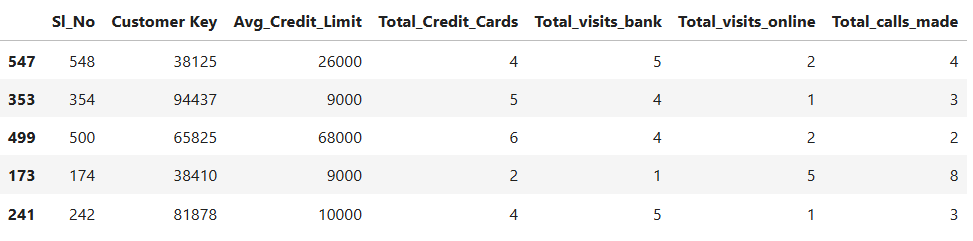
\includegraphics[width=0.85\textwidth]{dataset.png}
			\caption{A snapshot of data set used for analysis.}
			\label{fig:dataset}
		\end{figure}
		The data set consists of 660 records and 7 columns. I dropped two columns which represented unique customers and Serial number. Not useful for the analysis. After this we have 5 columns and all are numerical. No missing value or irregular values
		were found. All the records were unique. My motivation is to cluster these customers based on this five dimensional data set. 
	\subsection{Univariate and Bivariate Analysis}
	The figure \ref{fig:Numerical variables distribution} shows the distribution of all 5 numerical variables in the dataset. It shows the Histogram on the top of which box plot is aligned with the same scale. Figure \ref{fig:box_Avg_Credit_Limit} shows the distribution of Average Credit Limit of customers. On average customers have a  limit of 34,574. The Mean is much higher than median which shows that the distribution is highly right skewed. There are many outliers on the higher end of limit.
	Figure \ref{fig:box_Total_Credit_Cards} the distribution of total number of credit card owned by the customers from AllLife Bank. 75\% of customers have 6 or less number of credit cards. The maximum number owned is 10.
	Figure \ref{fig:box_Total_visits_bank} shows the distribution of number of visits from the customers to bank. Maximum number of times visited is 5. Figure \ref{fig:box_Total_visits_online} shows the distribution for online visits to banks websites and services. 75\% visited 5 times or less. But there are many outliers up to 15 times. Similarly from figure \ref{fig:box_Total_calls_made} we can see the distribution for number of phone calls made by the customers. 
	 
		\begin{figure}[h]
		\centering
		\begin{subfigure}[t]{0.49\textwidth}
			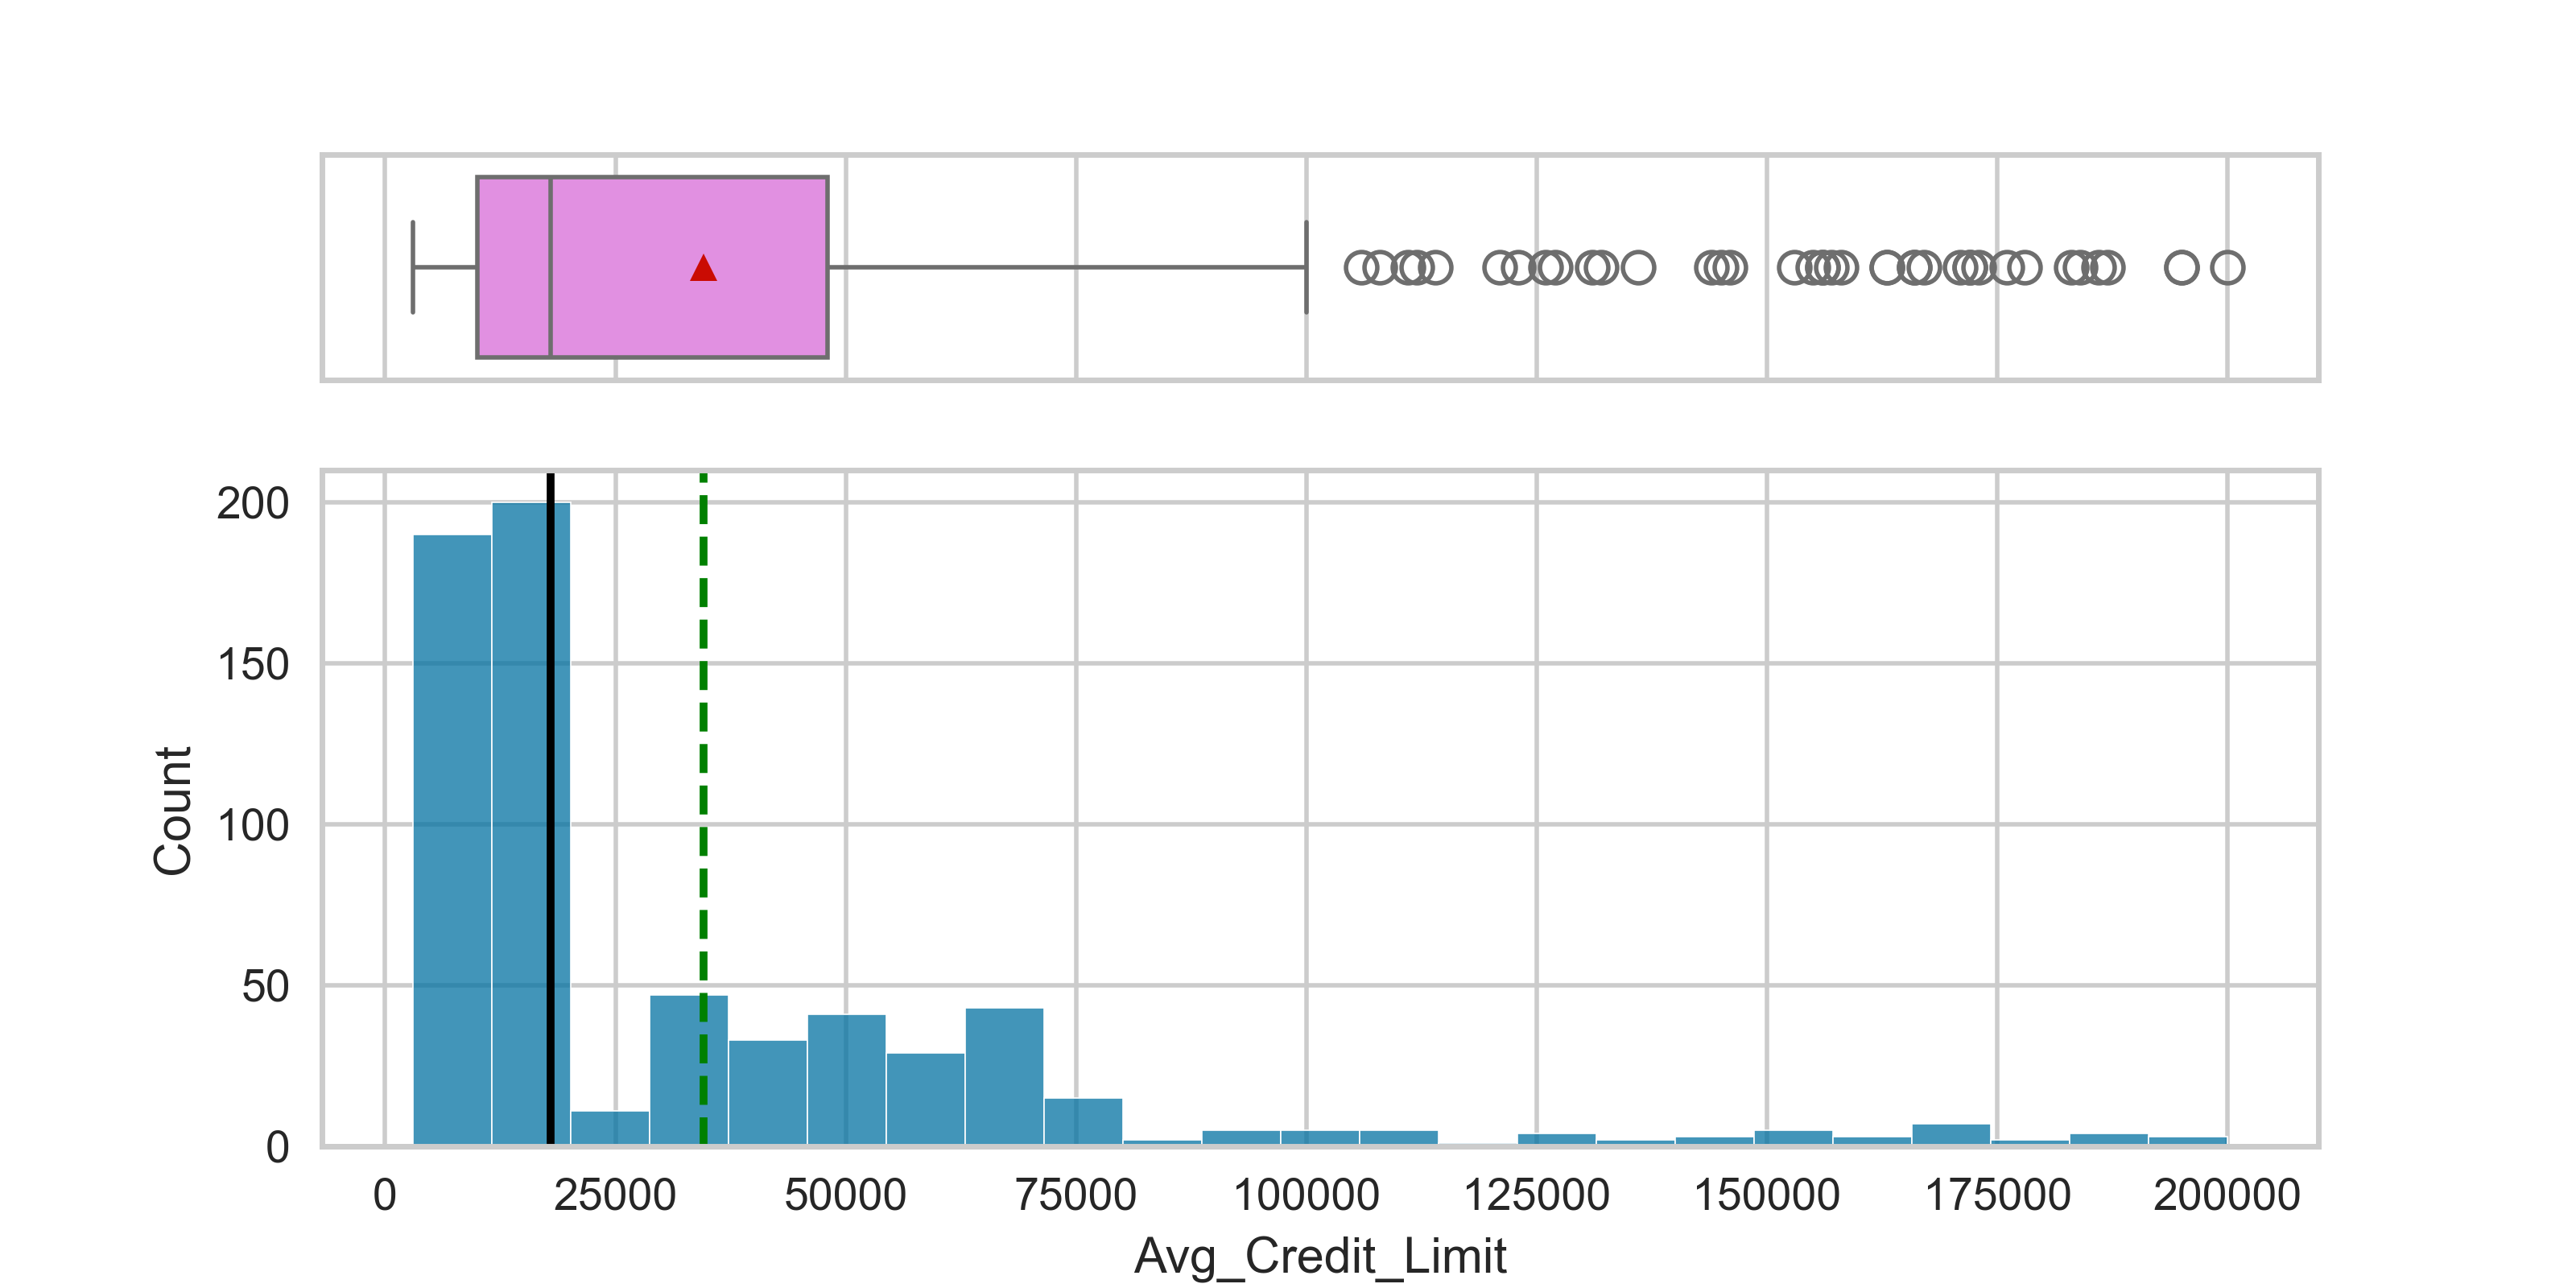
\includegraphics[width=\textwidth]{box_Avg_Credit_Limit.png}
			\caption{}
			\label{fig:box_Avg_Credit_Limit}
		\end{subfigure}
		\hfill
		\begin{subfigure}[t]{0.49\textwidth}
			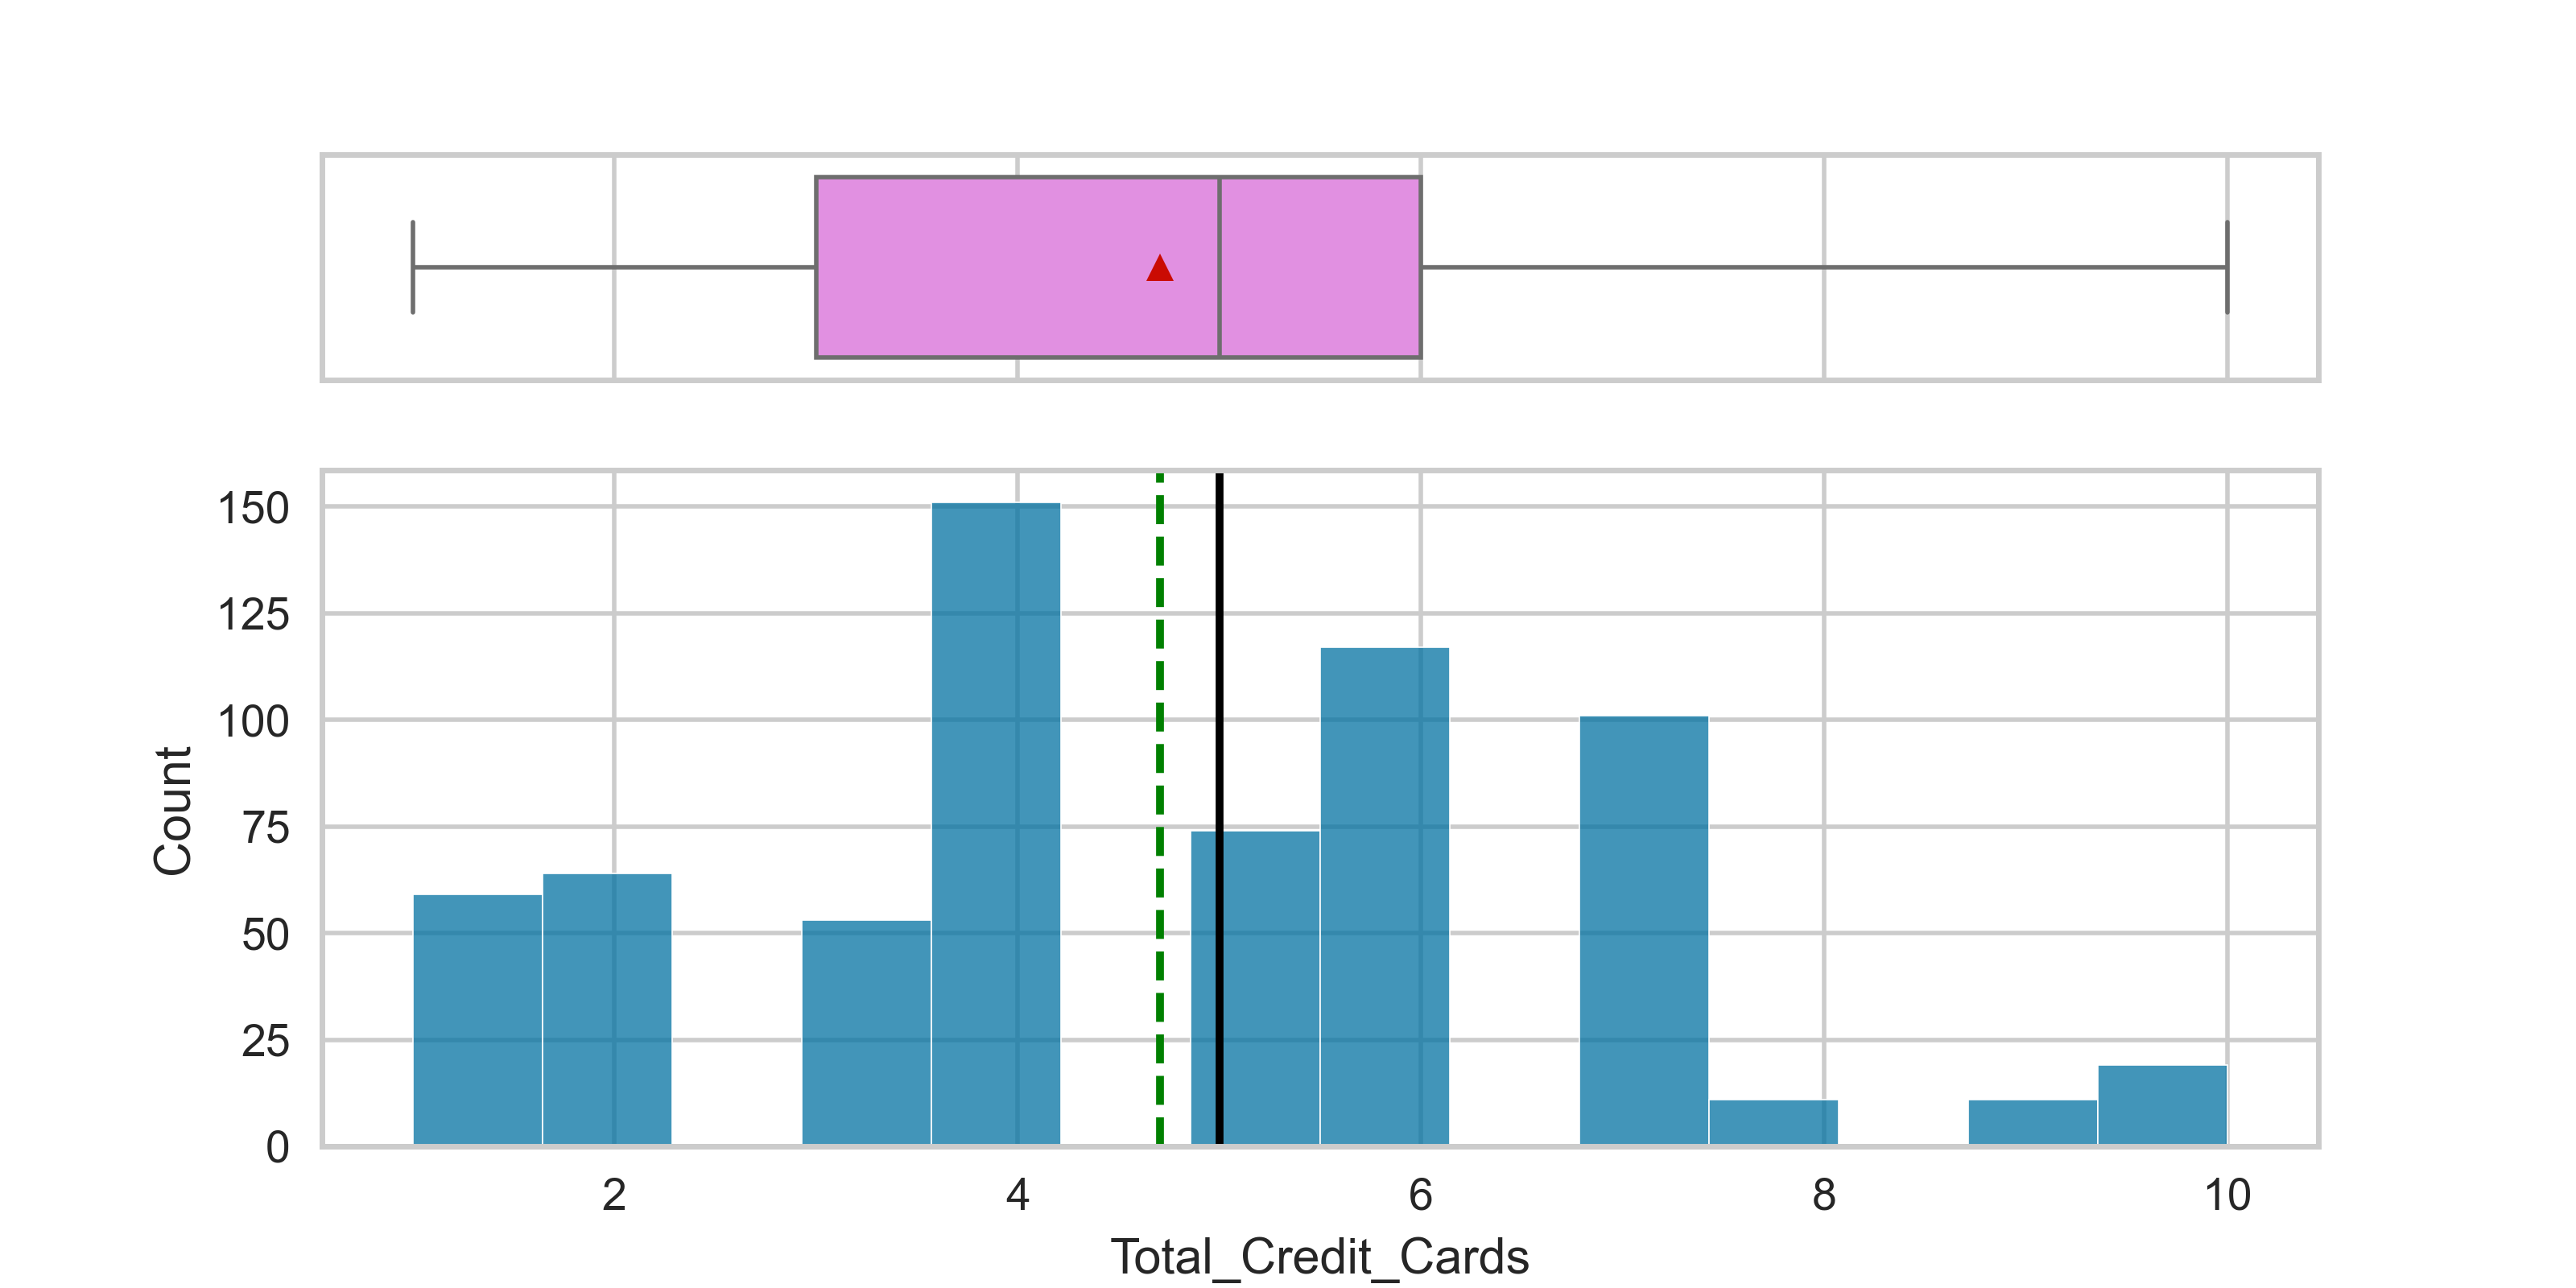
\includegraphics[width=\textwidth]{box_Total_Credit_Cards.png}
			\caption{}
			\label{fig:box_Total_Credit_Cards}
		\end{subfigure}
		\begin{subfigure}[t]{0.49\textwidth}
			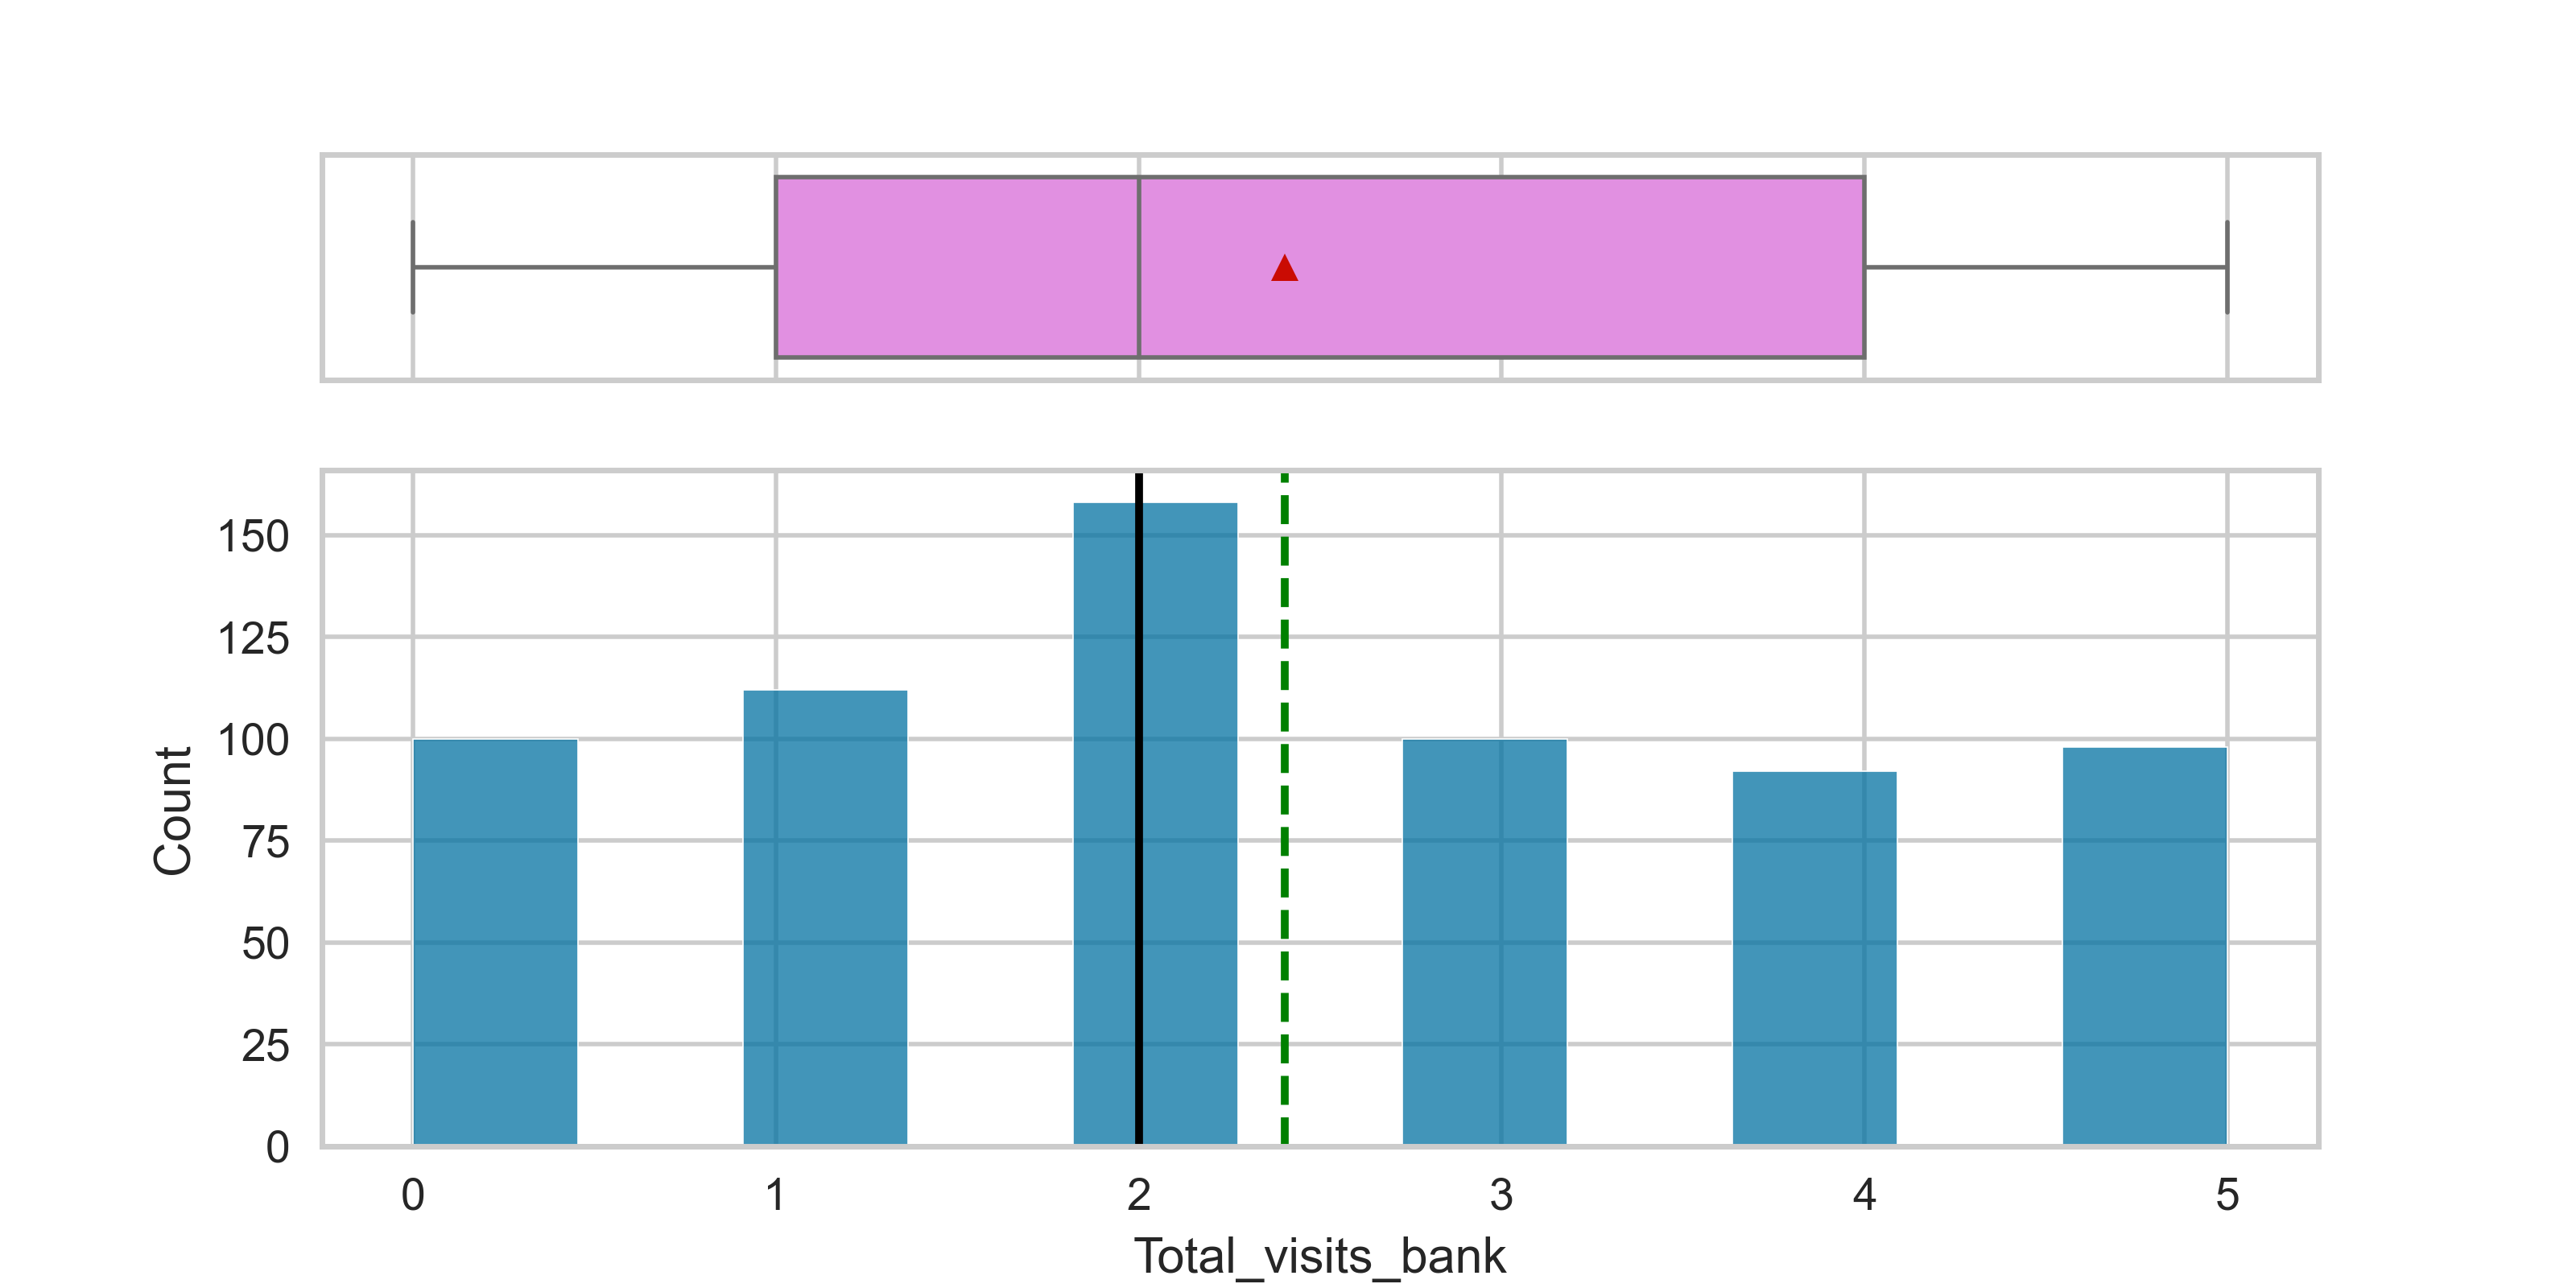
\includegraphics[width=\textwidth]{box_Total_visits_bank.png}
			\caption{}
			\label{fig:box_Total_visits_bank}
		\end{subfigure}
		\hfill
		\begin{subfigure}[t]{0.49\textwidth}
			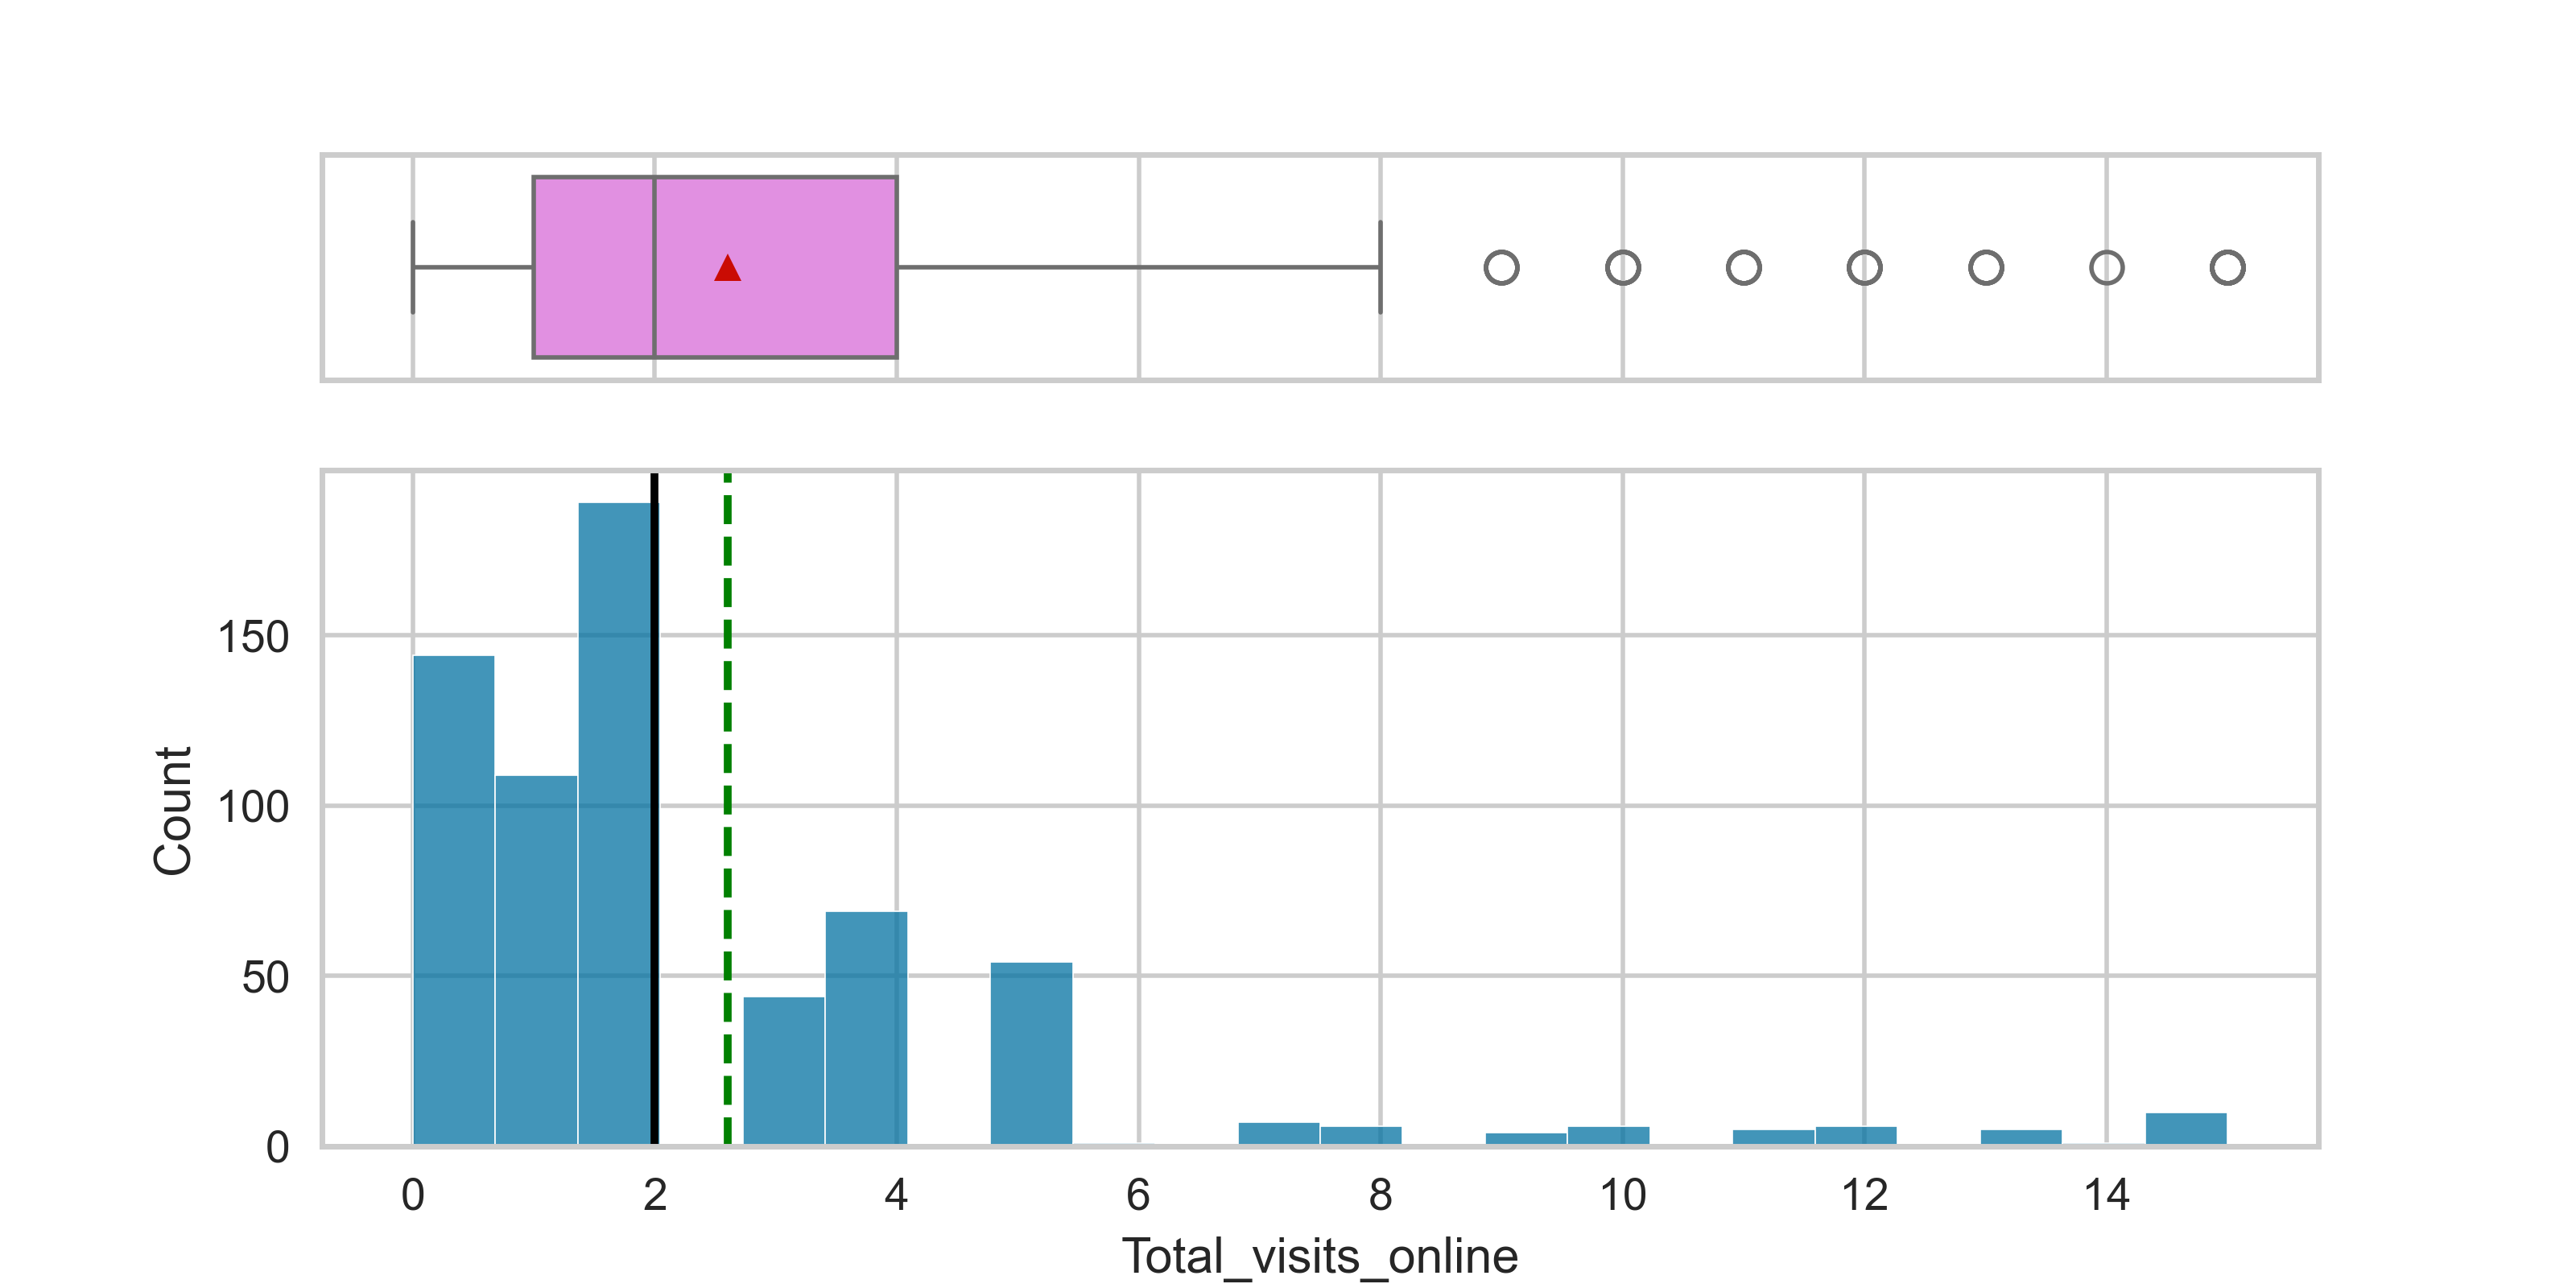
\includegraphics[width=\textwidth]{box_Total_visits_online.png}
			\caption{}
			\label{fig:box_Total_visits_online}
		\end{subfigure}
		\hfill
		\begin{subfigure}[t]{0.49\textwidth}
			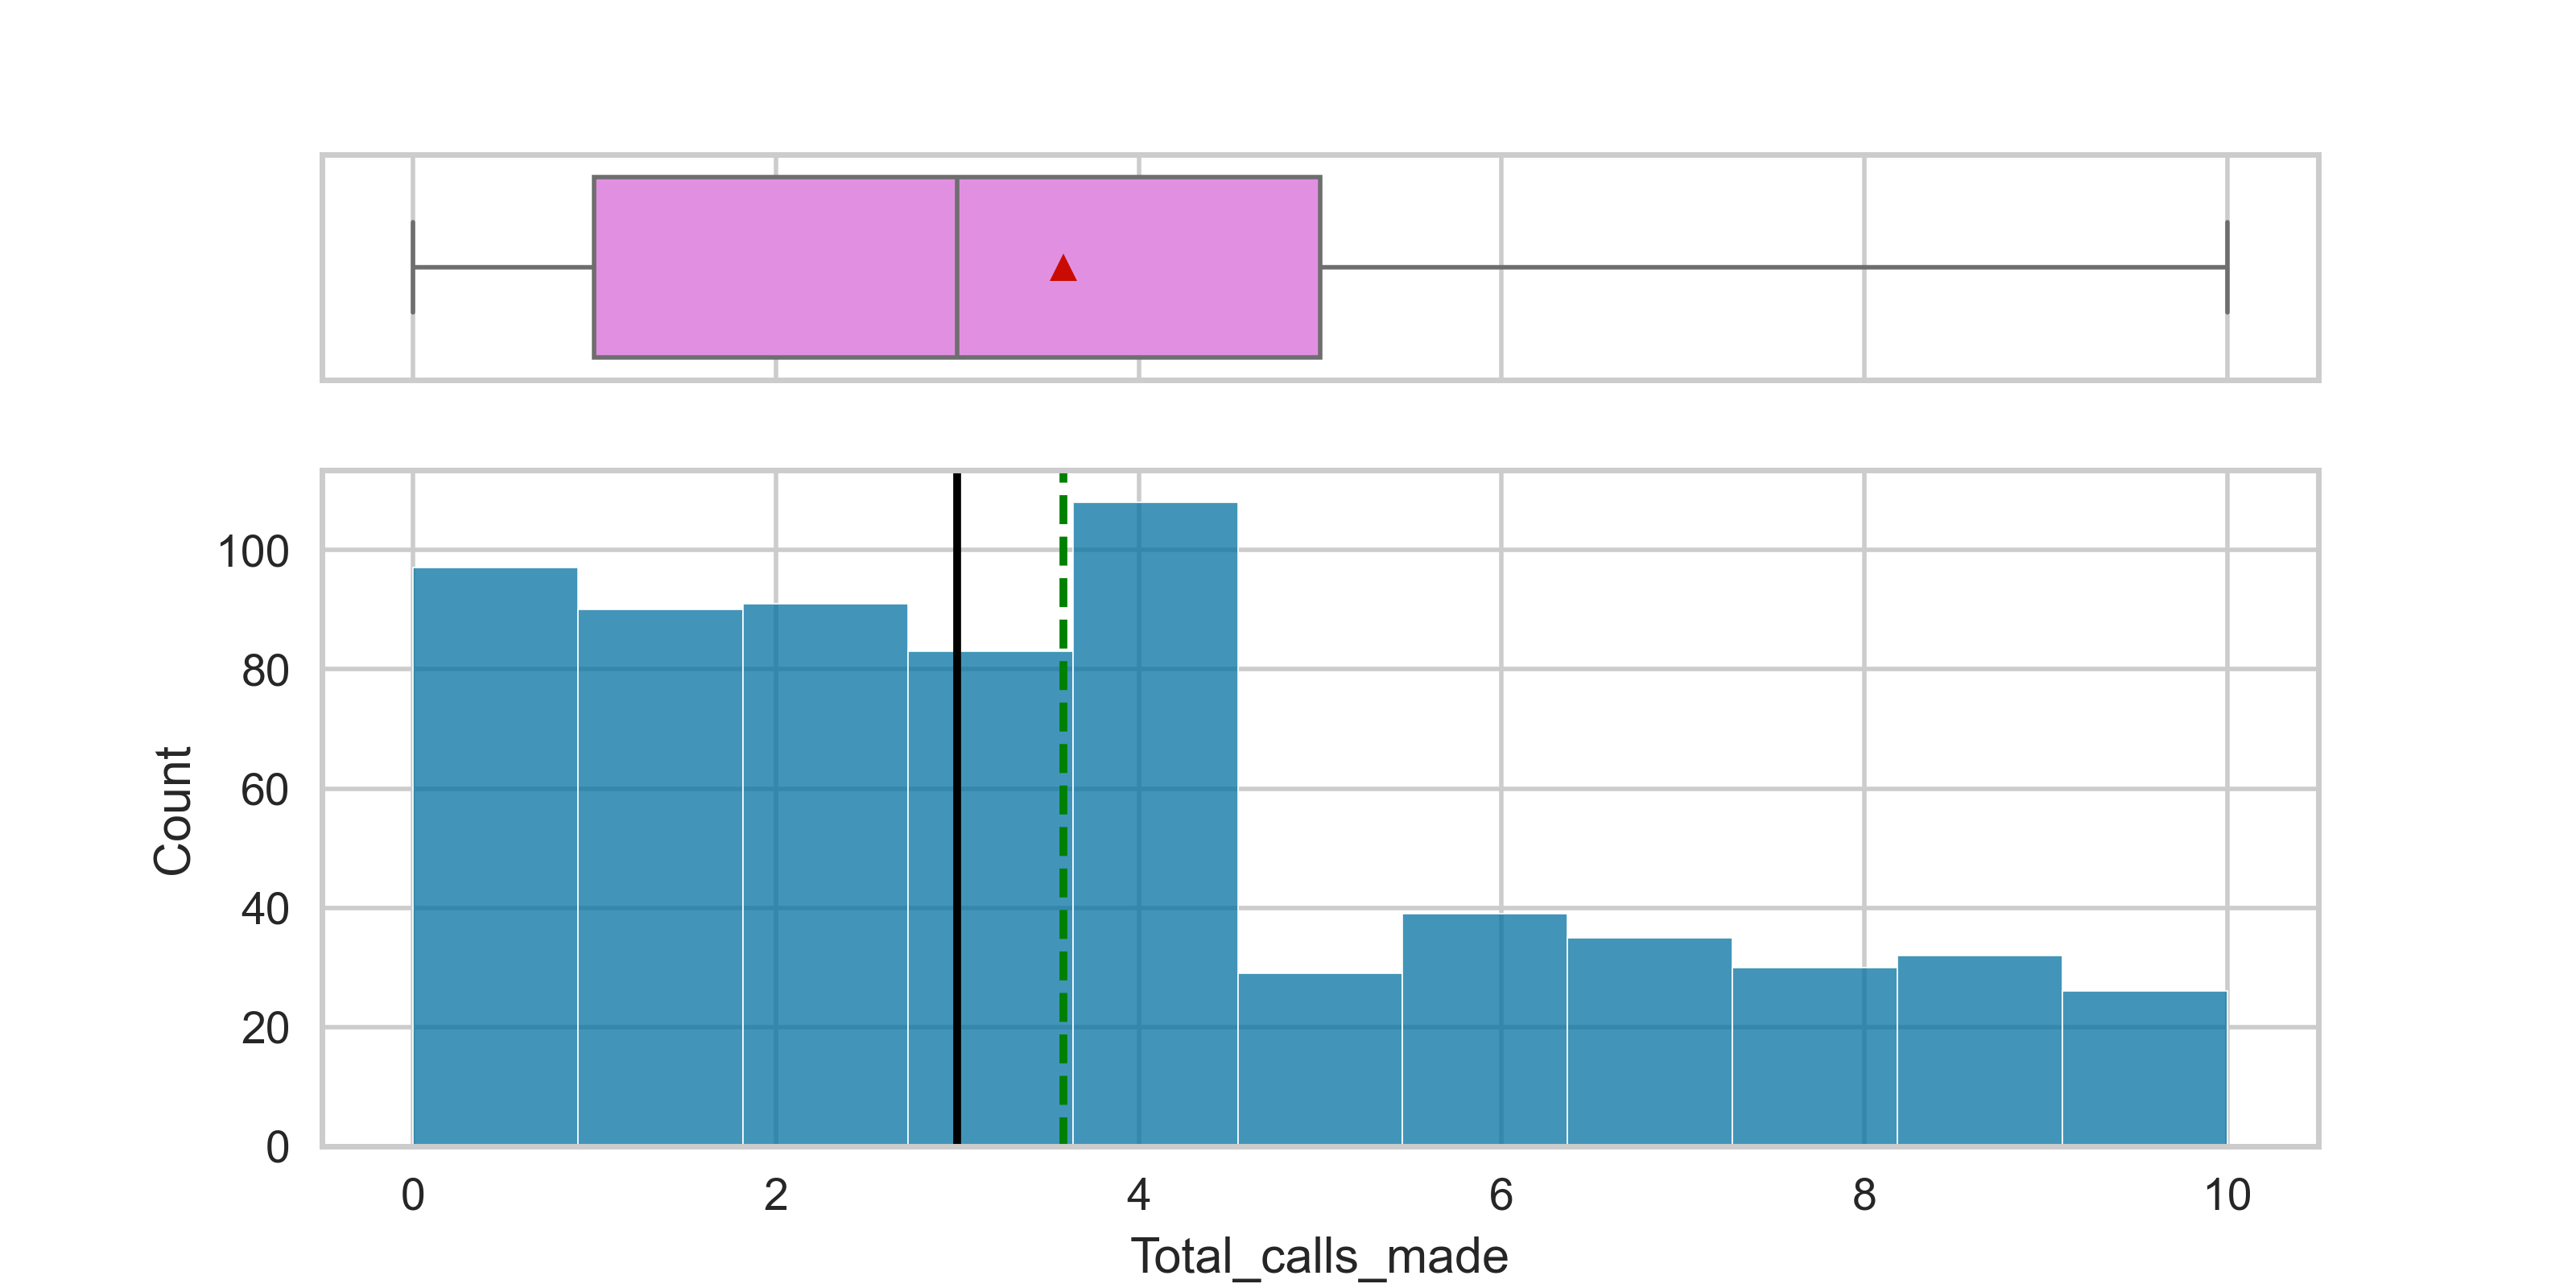
\includegraphics[width=\textwidth]{box_Total_calls_made.png}
			\caption{}
			\label{fig:box_Total_calls_made}
		\end{subfigure}
		\caption{Numerical variables distribution}
		\label{fig:Numerical variables distribution}
		\end{figure}	
		
		\begin{figure}[h]
			\centering
			\begin{subfigure}[t]{0.49\textwidth}
				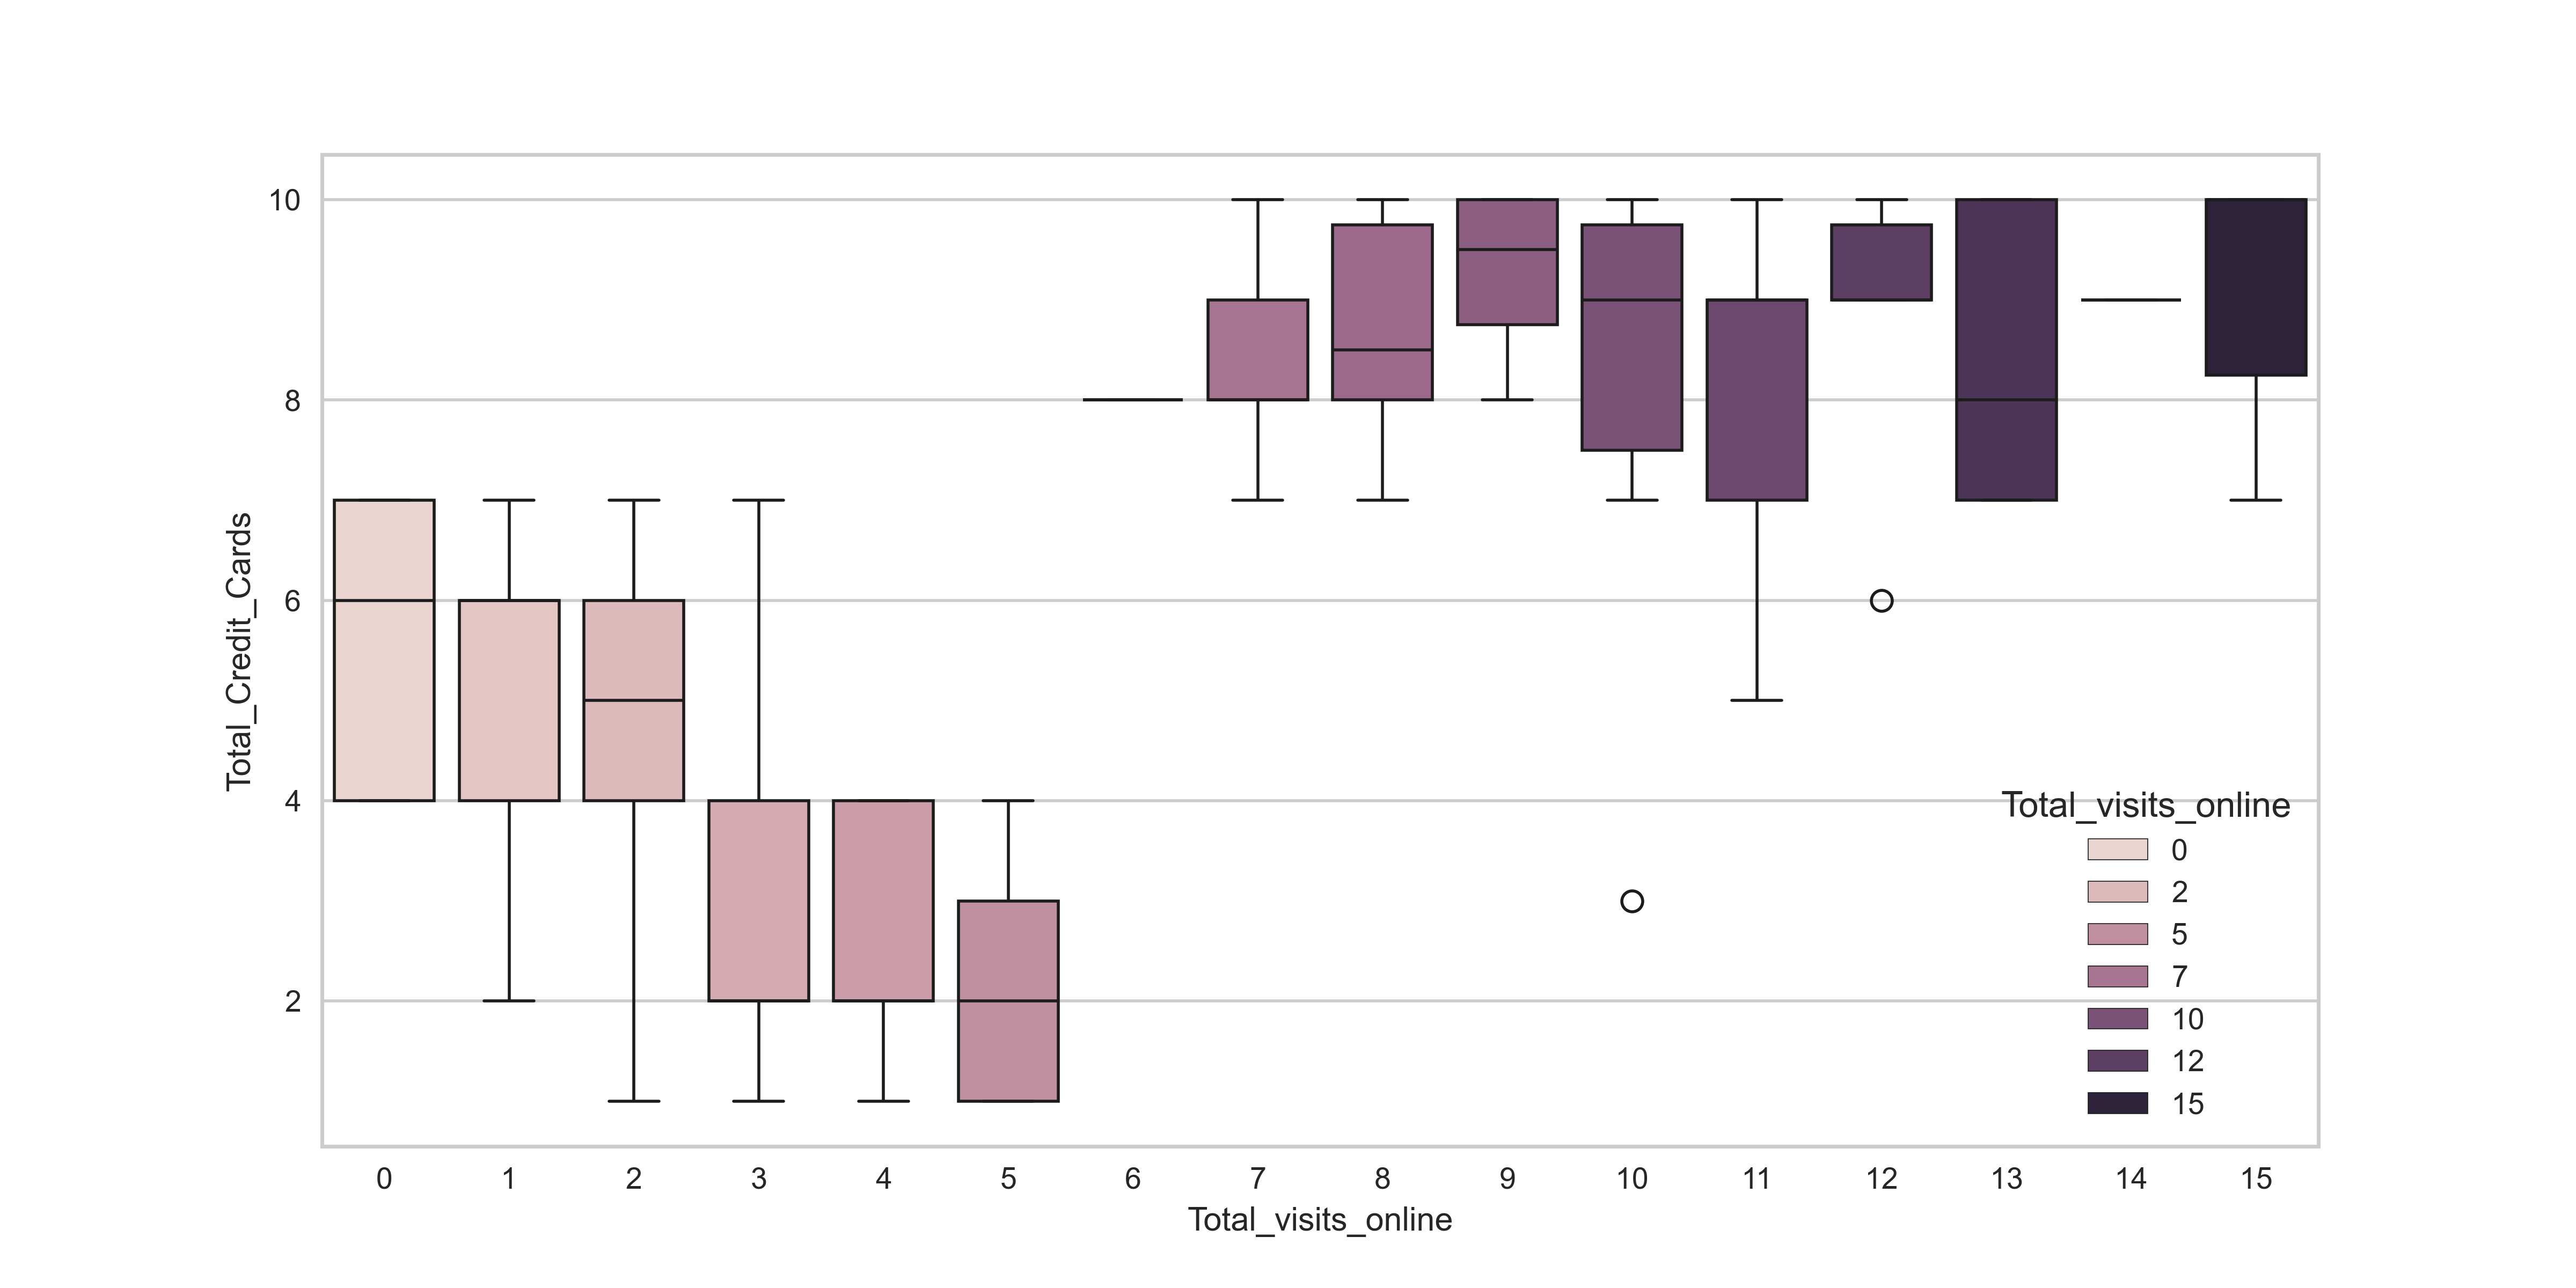
\includegraphics[width=\textwidth]{bi_box_Total_visits_online_Total_Credit_Cards.png}
				\caption{Total credit cards vs total online visits.}
				\label{fig:bi_box_Total_visits_online_Total_Credit_Cards}
			\end{subfigure}
			\hfill
			\begin{subfigure}[t]{0.49\textwidth}
				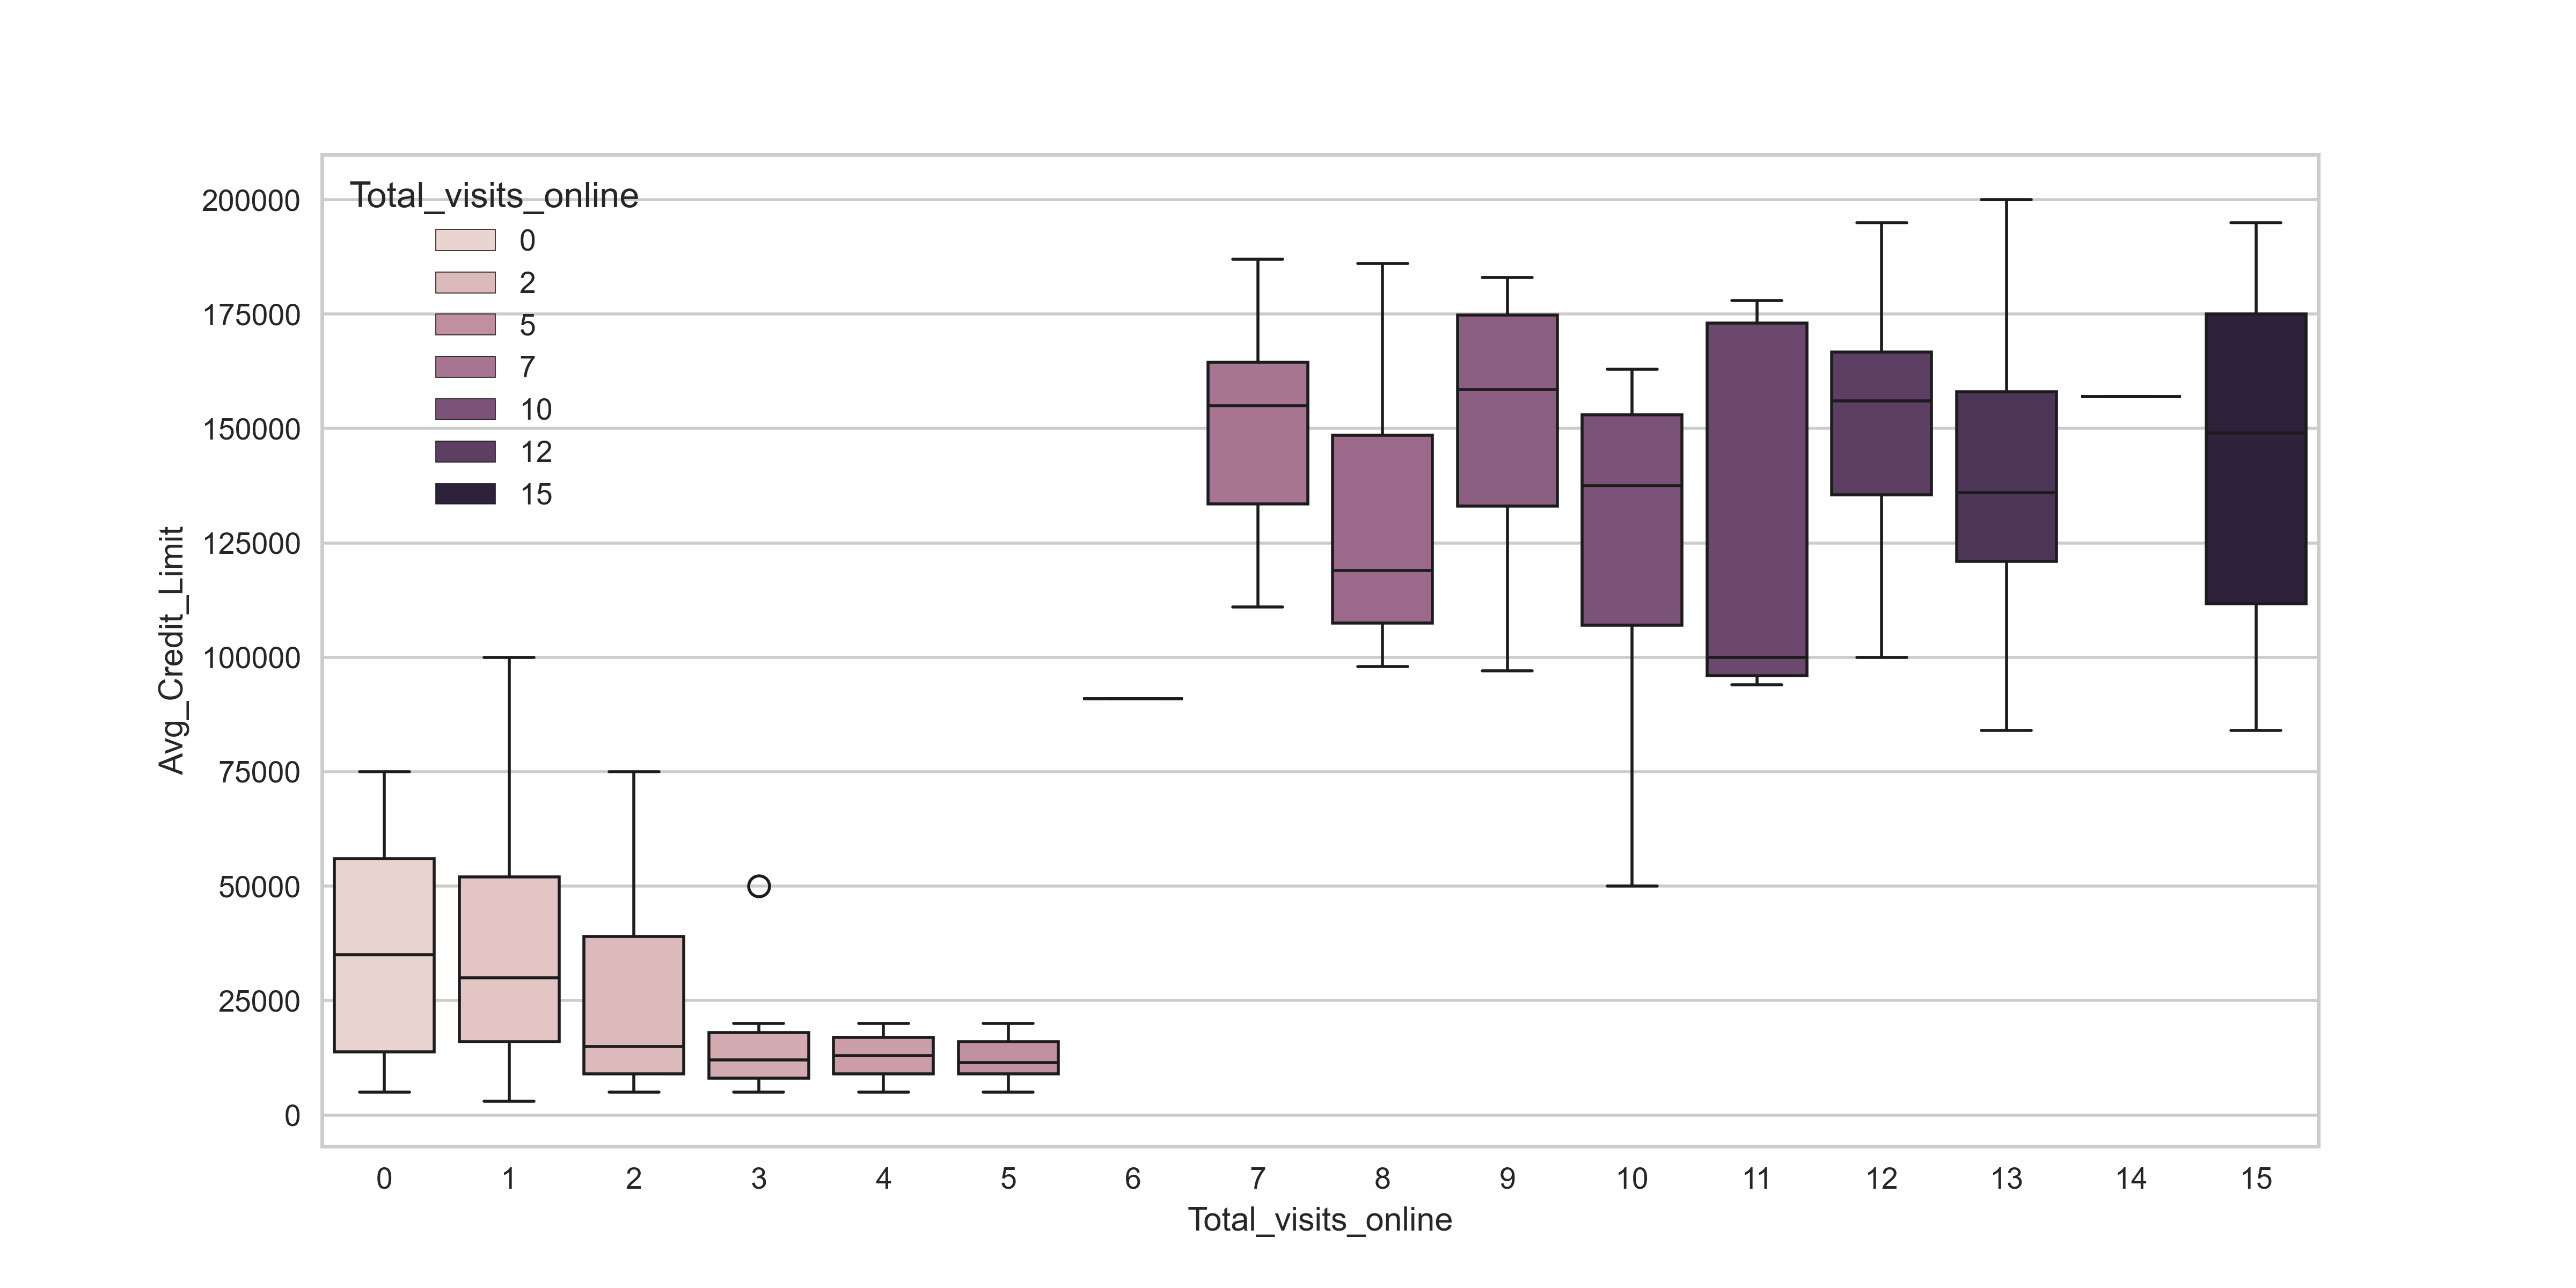
\includegraphics[width=\textwidth]{bi_box_Total_visits_online_Avg_Credit_Limit.png}
				\caption{Average credit limit vs Total online visits.}
				\label{fig:bi_box_Total_visits_online_Avg_Credit_Limit}
			\end{subfigure}
			\caption{Credit cards and average credit limits distribution with respect to online visits.}
			\label{fig:Credit cards and average credit limits distribution with respect to online visits}
		\end{figure}	
		
		
		\begin{figure}[h]
			\centering
			\begin{subfigure}[t]{0.49\textwidth}
				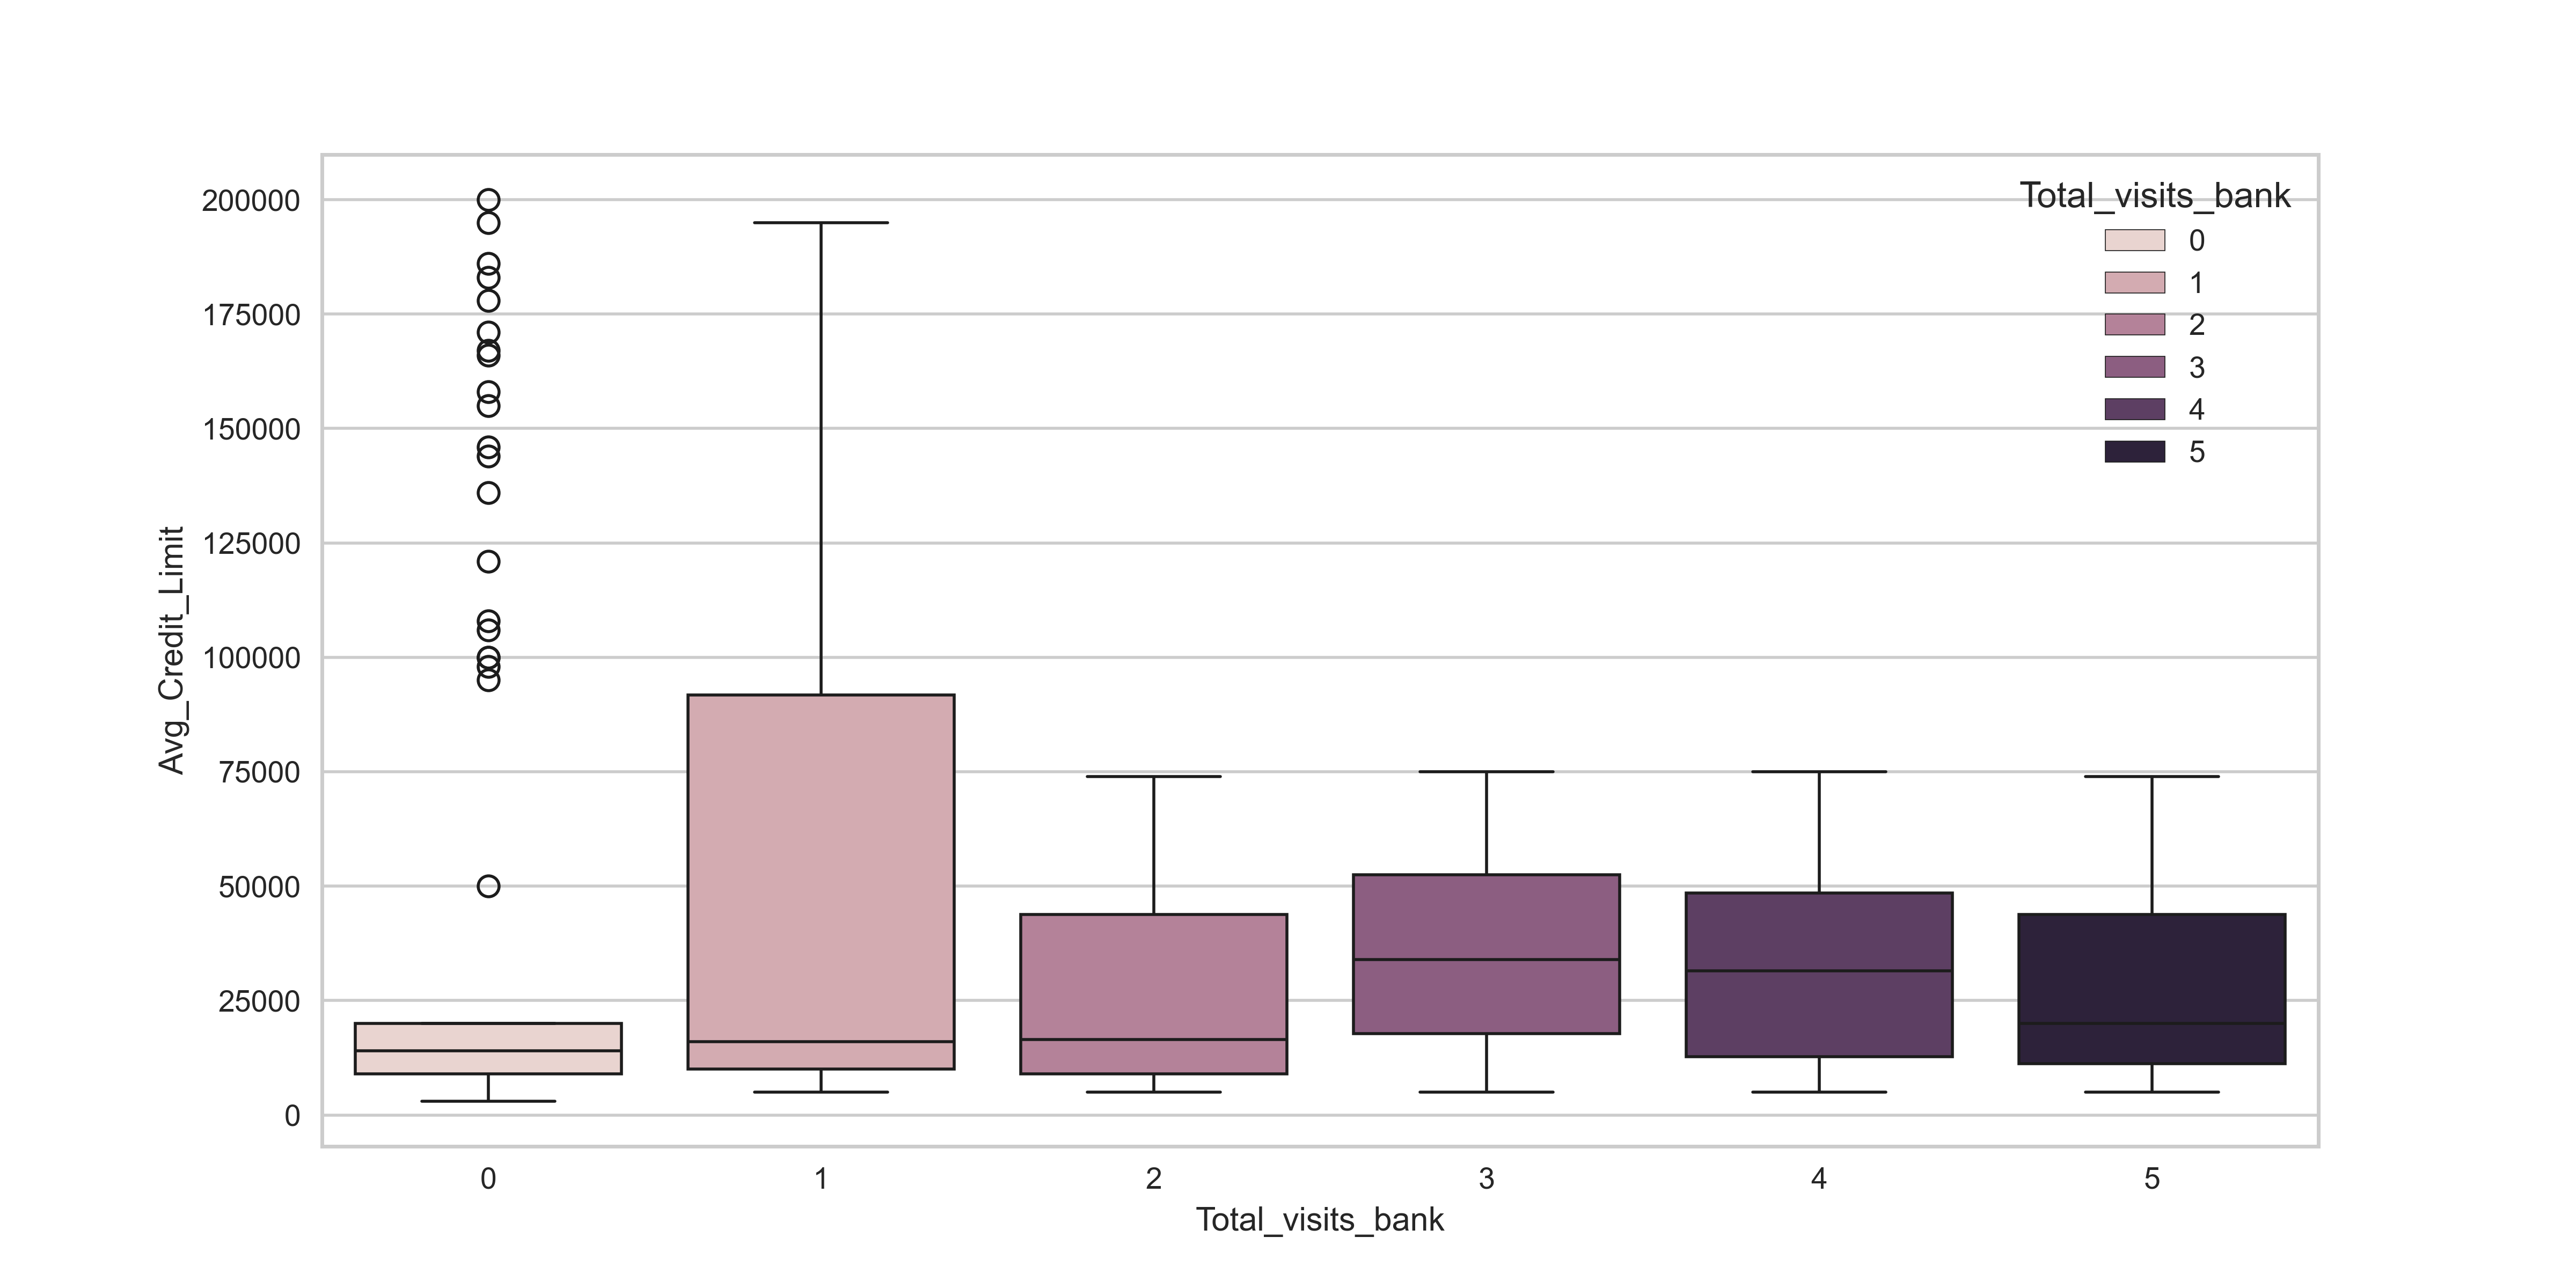
\includegraphics[width=\textwidth]{bi_box_Total_visits_bank_Avg_Credit_Limit.png}
				\caption{Average credit limit vs Total Bank visits.}
				\label{fig:bi_box_Total_visits_bank_Avg_Credit_Limit.pngs}
			\end{subfigure}
			\hfill
			\begin{subfigure}[t]{0.49\textwidth}
				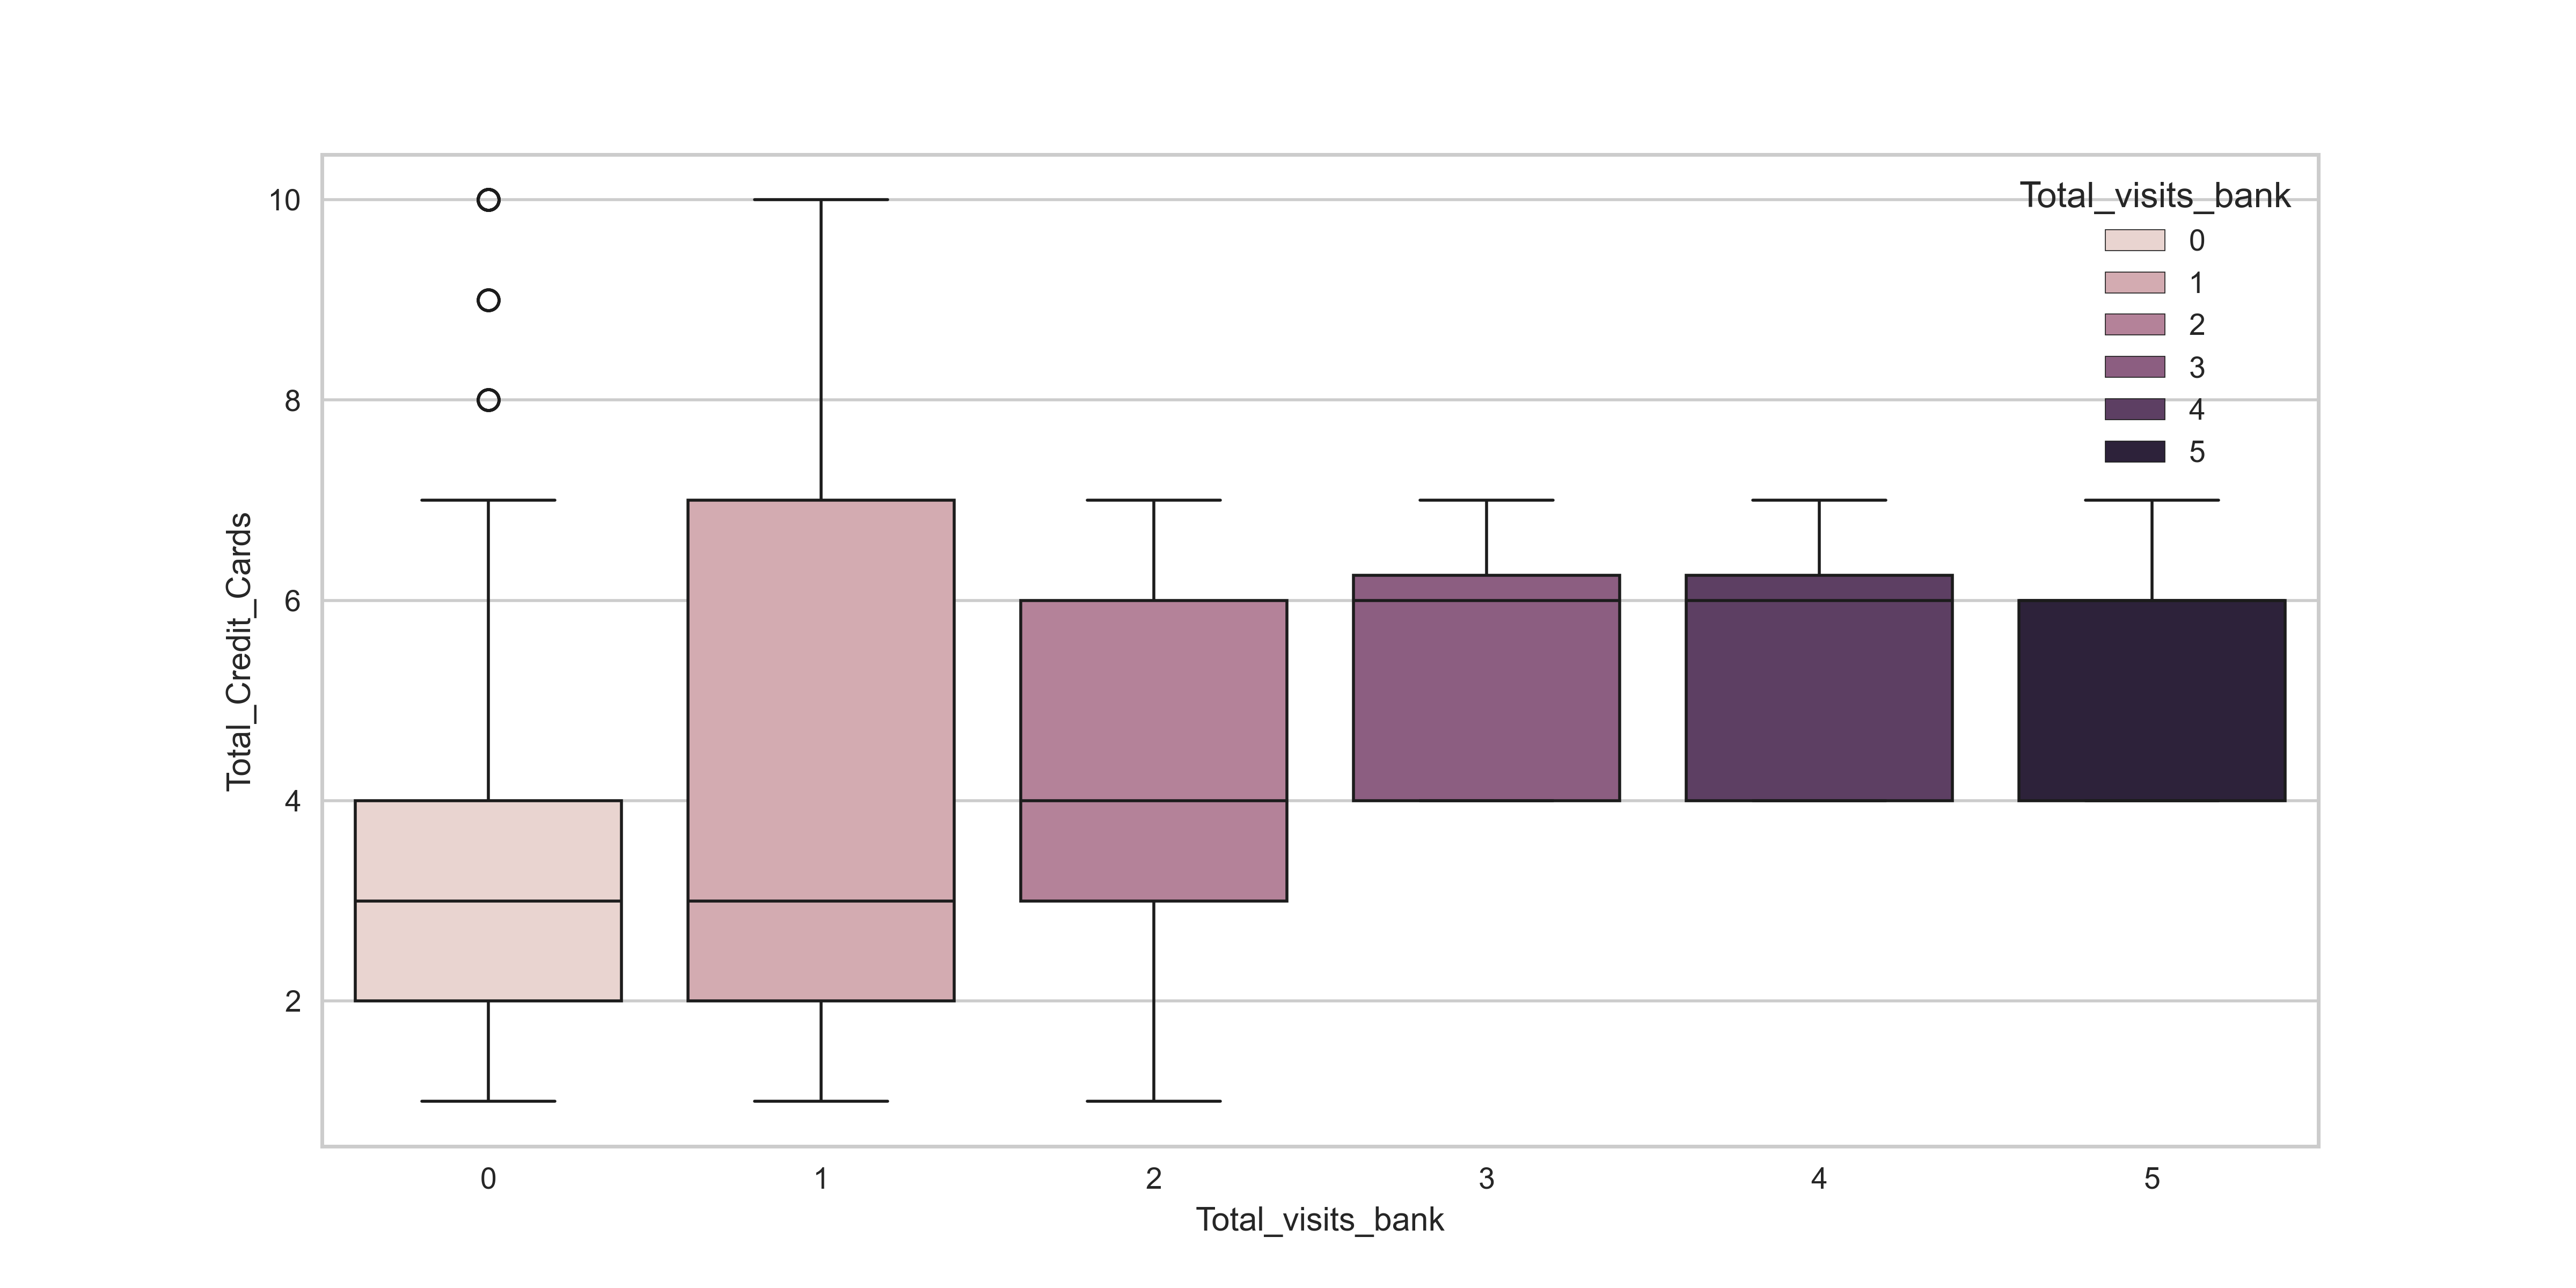
\includegraphics[width=\textwidth]{bi_box_Total_visits_bank_Total_Credit_Cards.png}
				\caption{Total credit cards vs total Bank visits.}
				\label{fig:bi_box_Total_visits_bank_Total_Credit_Cards.png}
			\end{subfigure}
			\caption{Credit cards and average credit limits distribution with respect to Bank visits.}
			\label{fig:Credit cards and average credit limits distribution with respect to Bank visits}
		\end{figure}
		
		\begin{figure}[h]
			\centering
			\begin{subfigure}[t]{0.49\textwidth}
				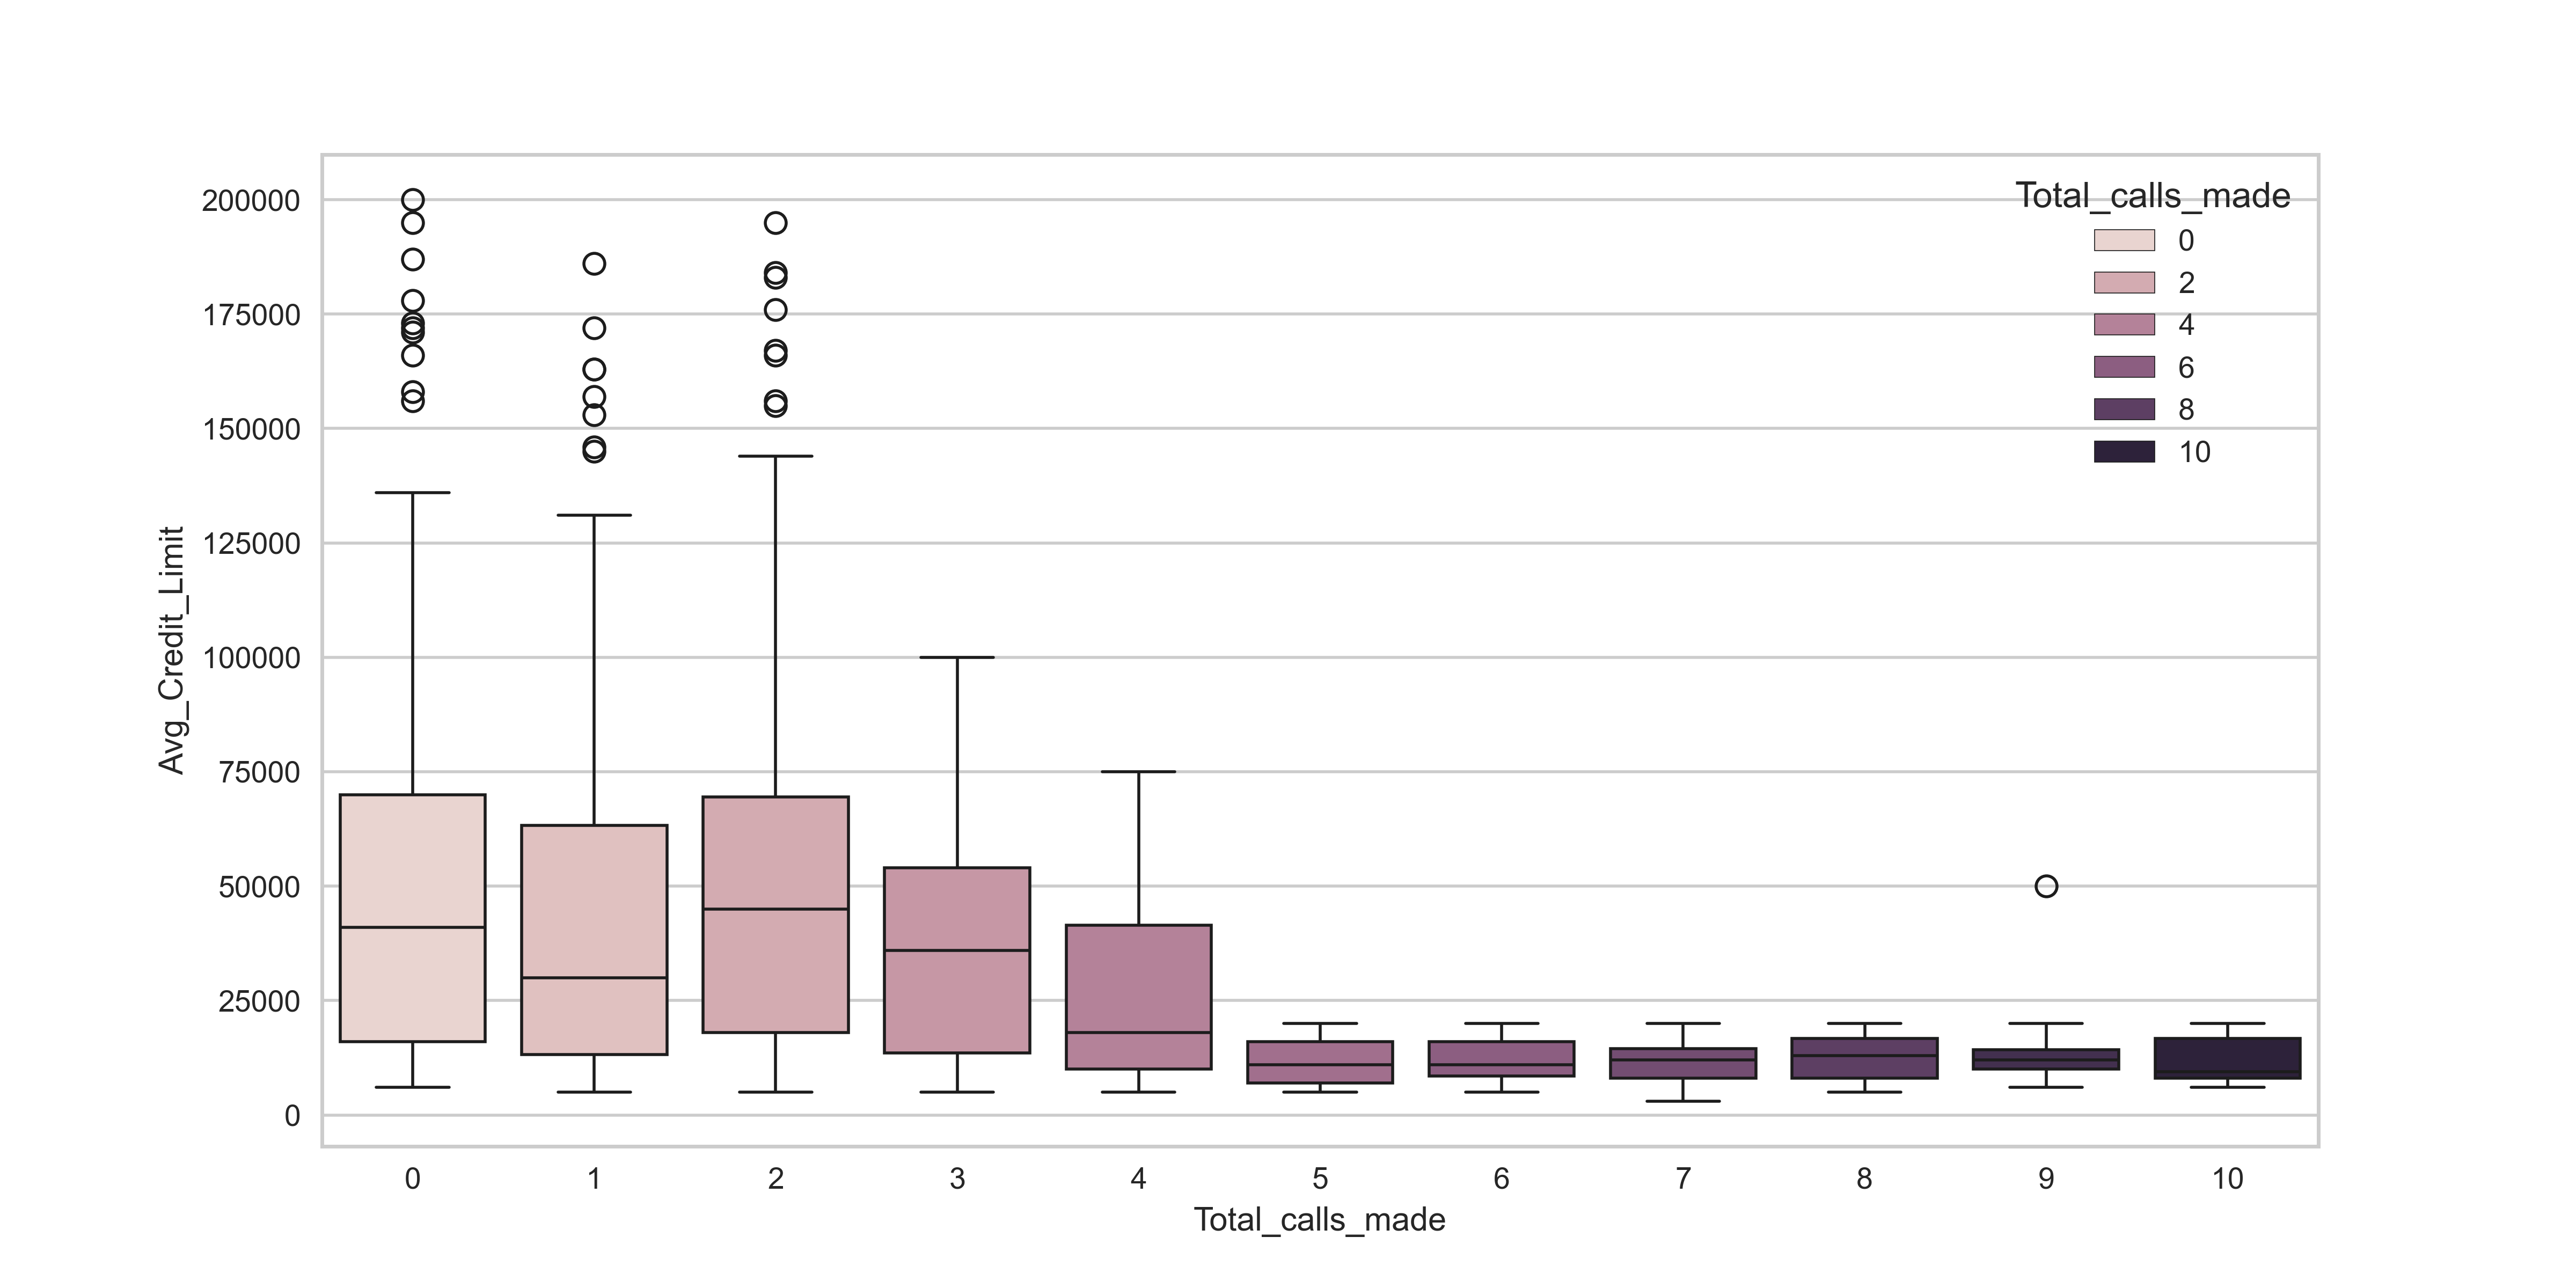
\includegraphics[width=\textwidth]{bi_box_Total_calls_made_Avg_Credit_Limit.png}
				\caption{Average credit limit vs Total calls made.}
				\label{fig:bi_box_Total_calls_made_Avg_Credit_Limit.png}
			\end{subfigure}
			\hfill
			\begin{subfigure}[t]{0.49\textwidth}
				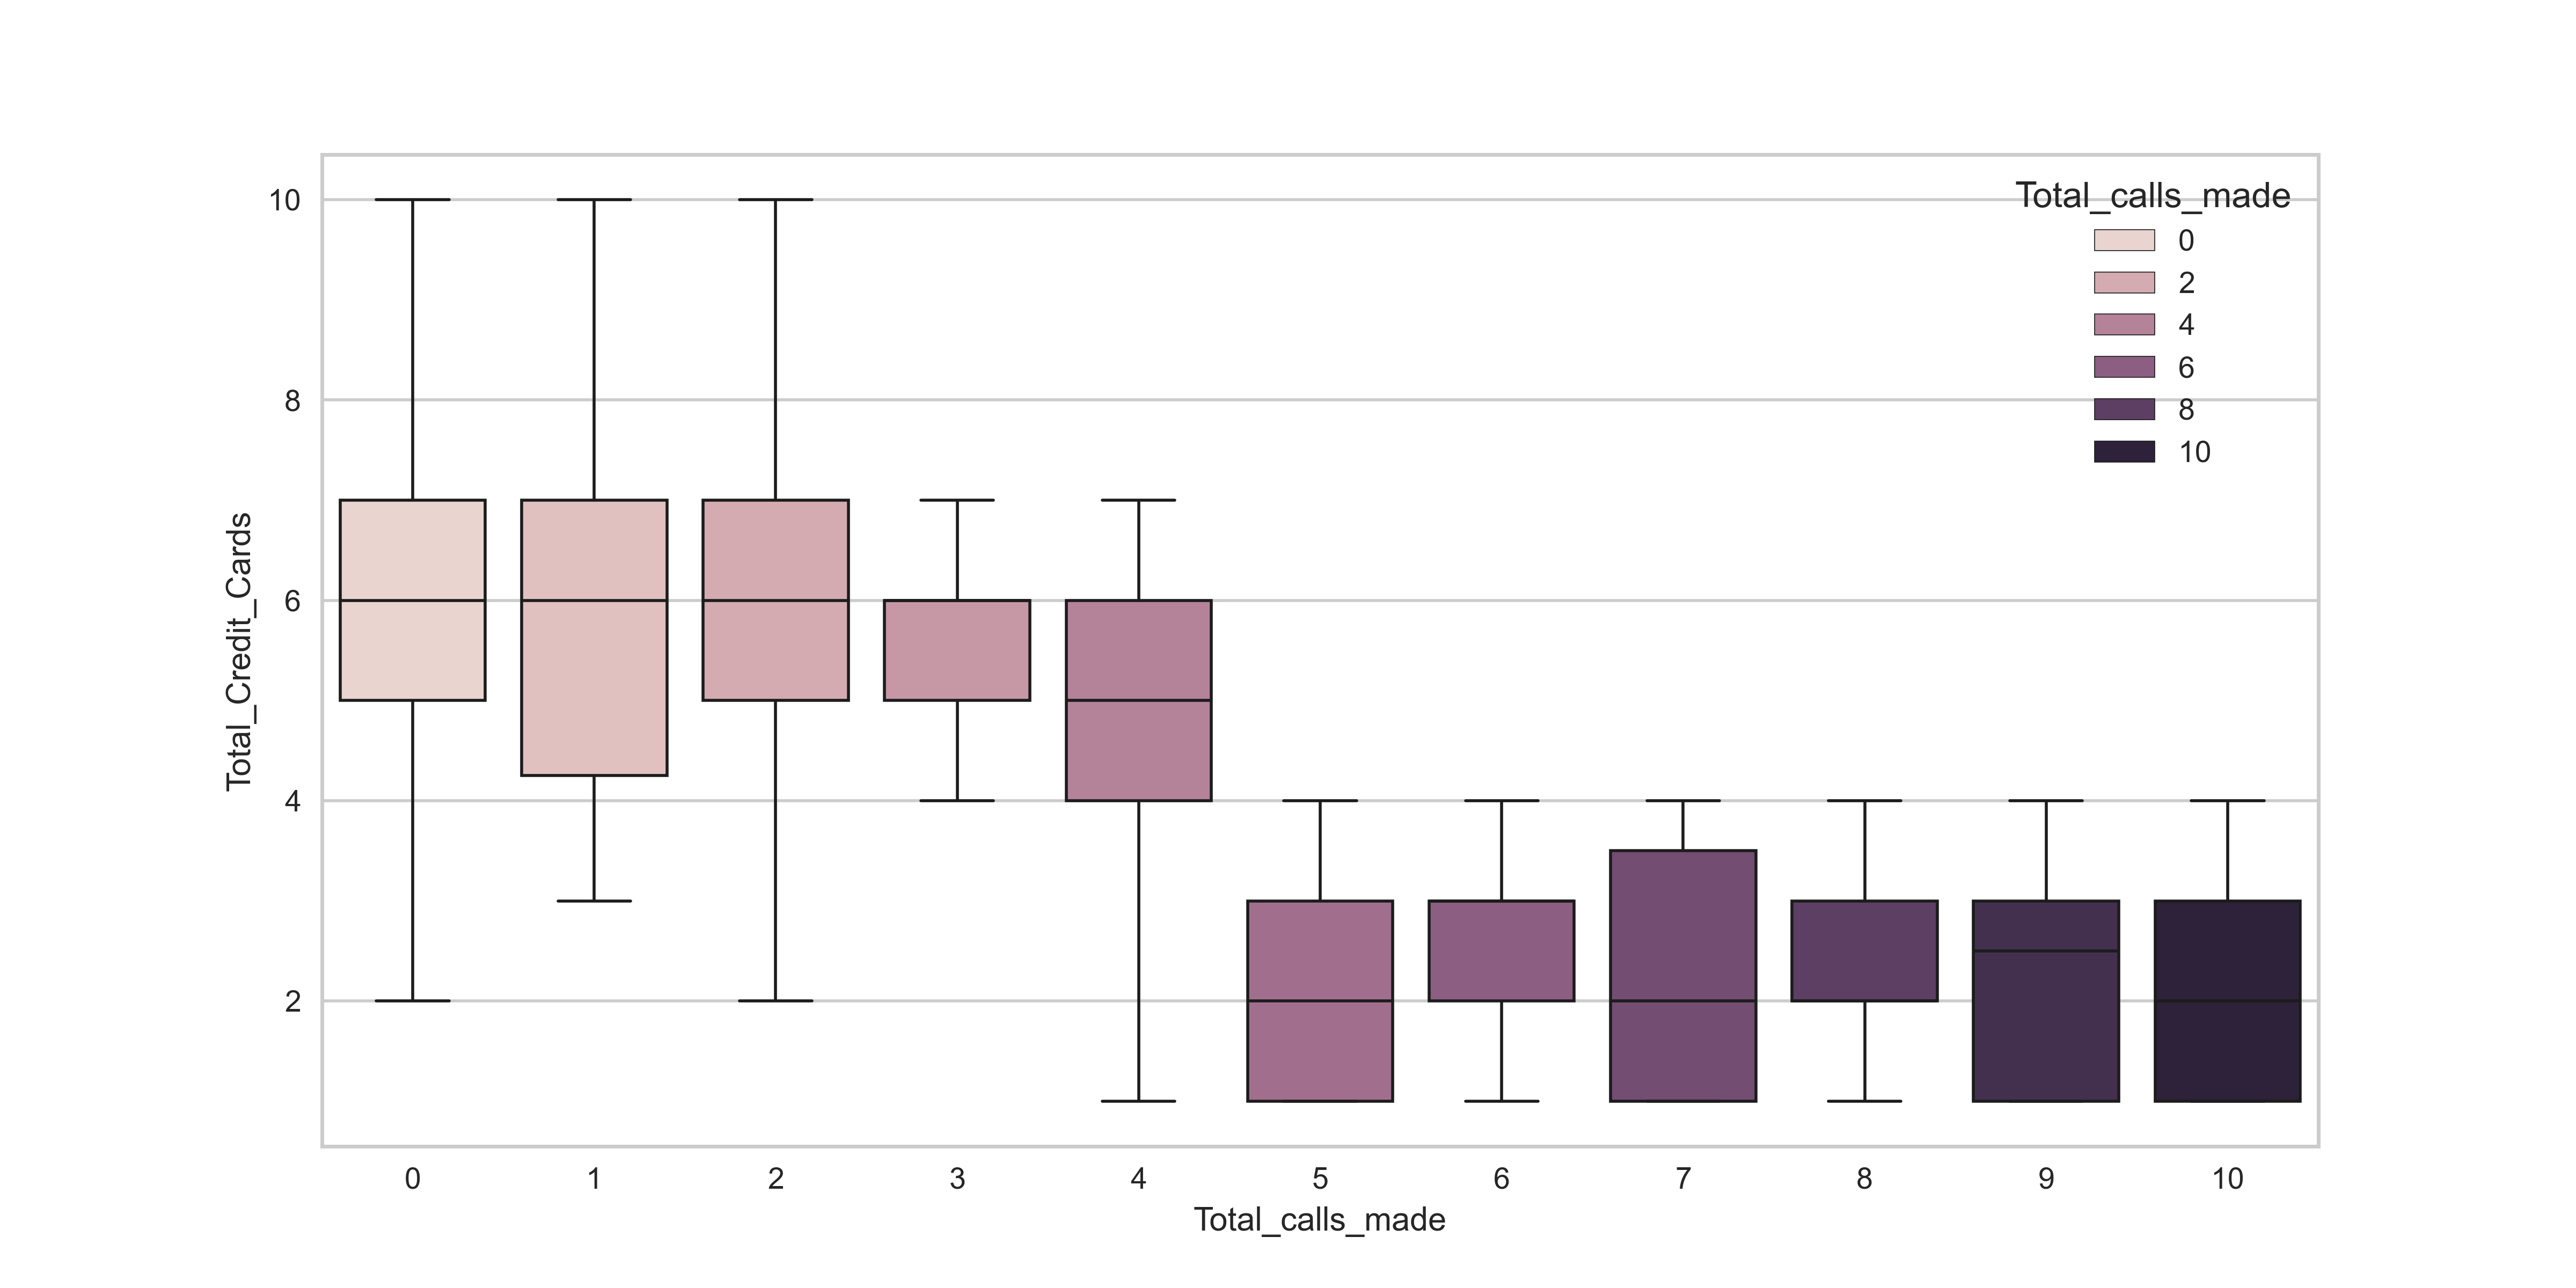
\includegraphics[width=\textwidth]{bi_box_Total_calls_madek_Total_Credit_Cards.png}
				\caption{Total credit cards vs total calls made.}
				\label{fig:bi_box_Total_calls_madek_Total_Credit_Cards.pngt}
			\end{subfigure}
			\caption{Credit cards and average credit limits distribution with respect to Number of calls made.}
			\label{fig:Credit cards and average credit limits distribution with respect to Number of calls made.}
		\end{figure}
		I tried to investigate how number of cards and credit limit owned by the customers varied with respect to how many times they contacted or visited bank through different channels. Figure \ref{fig:Credit cards and average credit limits distribution with respect to online visits}  shows the  Credit cards and average credit limits distribution with respect to online visits. We observe that customer visits higher than 6 have significantly higher number of credit cards and limit. In fact from this plot we sort of get a glimpse into two major clusters. Therefore online visit is a good segregate variable for different customers group.
		Figure \ref{fig:Credit cards and average credit limits distribution with respect to Bank visits} shows the Credit cards and average credit limits distribution with respect to Bank visits. We observe that the variation is more pronounced for Total number of credit cards. Customers with higher number of cards made more visits to Banks which is expected since more the cards the more maintenance and services one might need. Similar story is also observed for the Total calls made in case of Number of credit cards as shown in figure \ref{fig:Credit cards and average credit limits distribution with respect to Number of calls made.} which depicts Credit cards and average credit limits distribution with respect to Number of calls made.
		
		\begin{figure}[h]
			\centering
			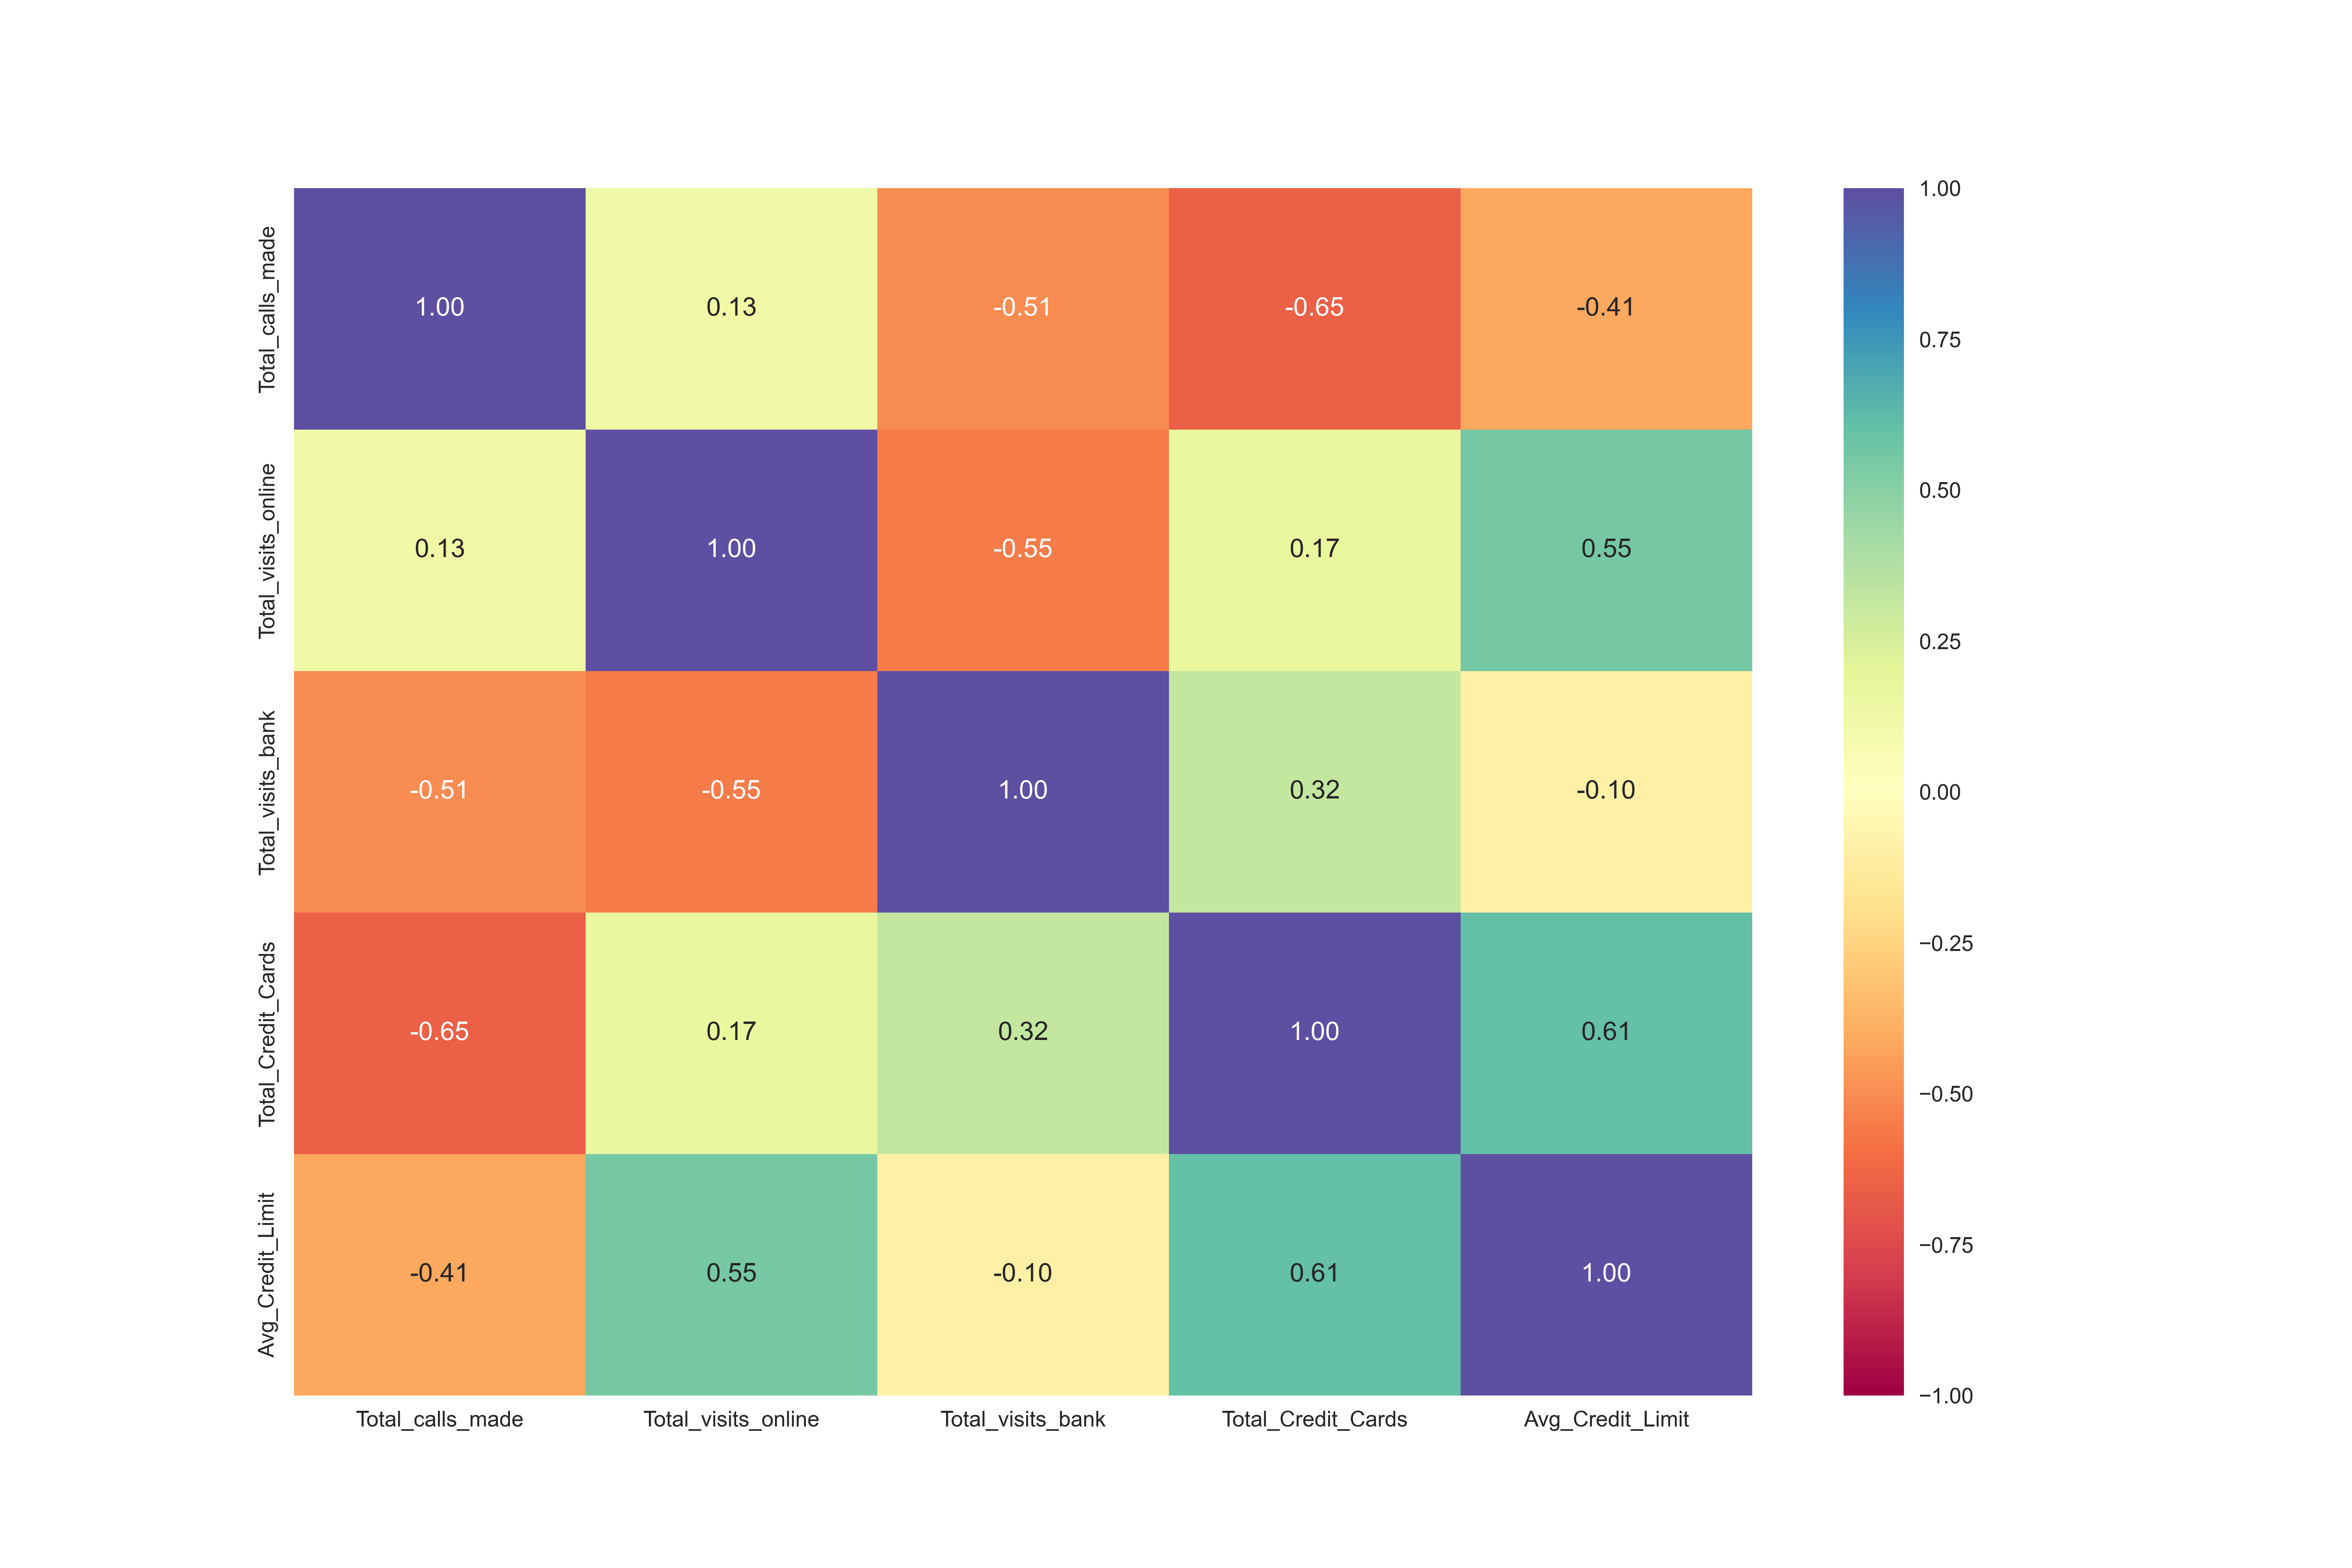
\includegraphics[width=\textwidth,height=10 cm]{corr.png}
			\caption{Correlation among the variables.}
			\label{fig:corrt}
		\end{figure}
		Figure \ref{fig:corrt} shows the heat map for the correlation among five variables. Bank visits and Online visits are negatively correlated with -0.55. This shows that customers using online services/modes are less likely to visit the bank in person. we also observe that number of credit cards and number of phone calls are negatively correlated with -0.65. In contrast to this number of credit cards is positively correlated to online visits. Customers with higher credit cards and limit are more likely to use online methods.
	\clearpage	
	\section{Data Preprocessing}
		Data preprocessing is a crucial step in clustering to ensure that the data is clean, consistent, and suitable for analysis. The data set did not have any irregular or missing values. As for the outliers that we found in credit limit and online visits, it would not have been a good choice to remove these, since all of these records are valid and also no instability was found during clustering implementation due to these outliers which off course if described posterior to implementation. Normalization of the data ensures that all features contribute equally to the distance calculations. Common methods include Min-Max scaling and Z-score normalization. I carried out the Z-score on all the five features since the range of values for credit limit is significantly higher than all other columns. This was necessary to avoid bias to any particular feature. After the transformation the normalized dataset is shown in distribution plot figure \ref{fig:scaled_data}. We see that all the features are now centered around the mean zero.
		\begin{figure}[h]
			\centering
			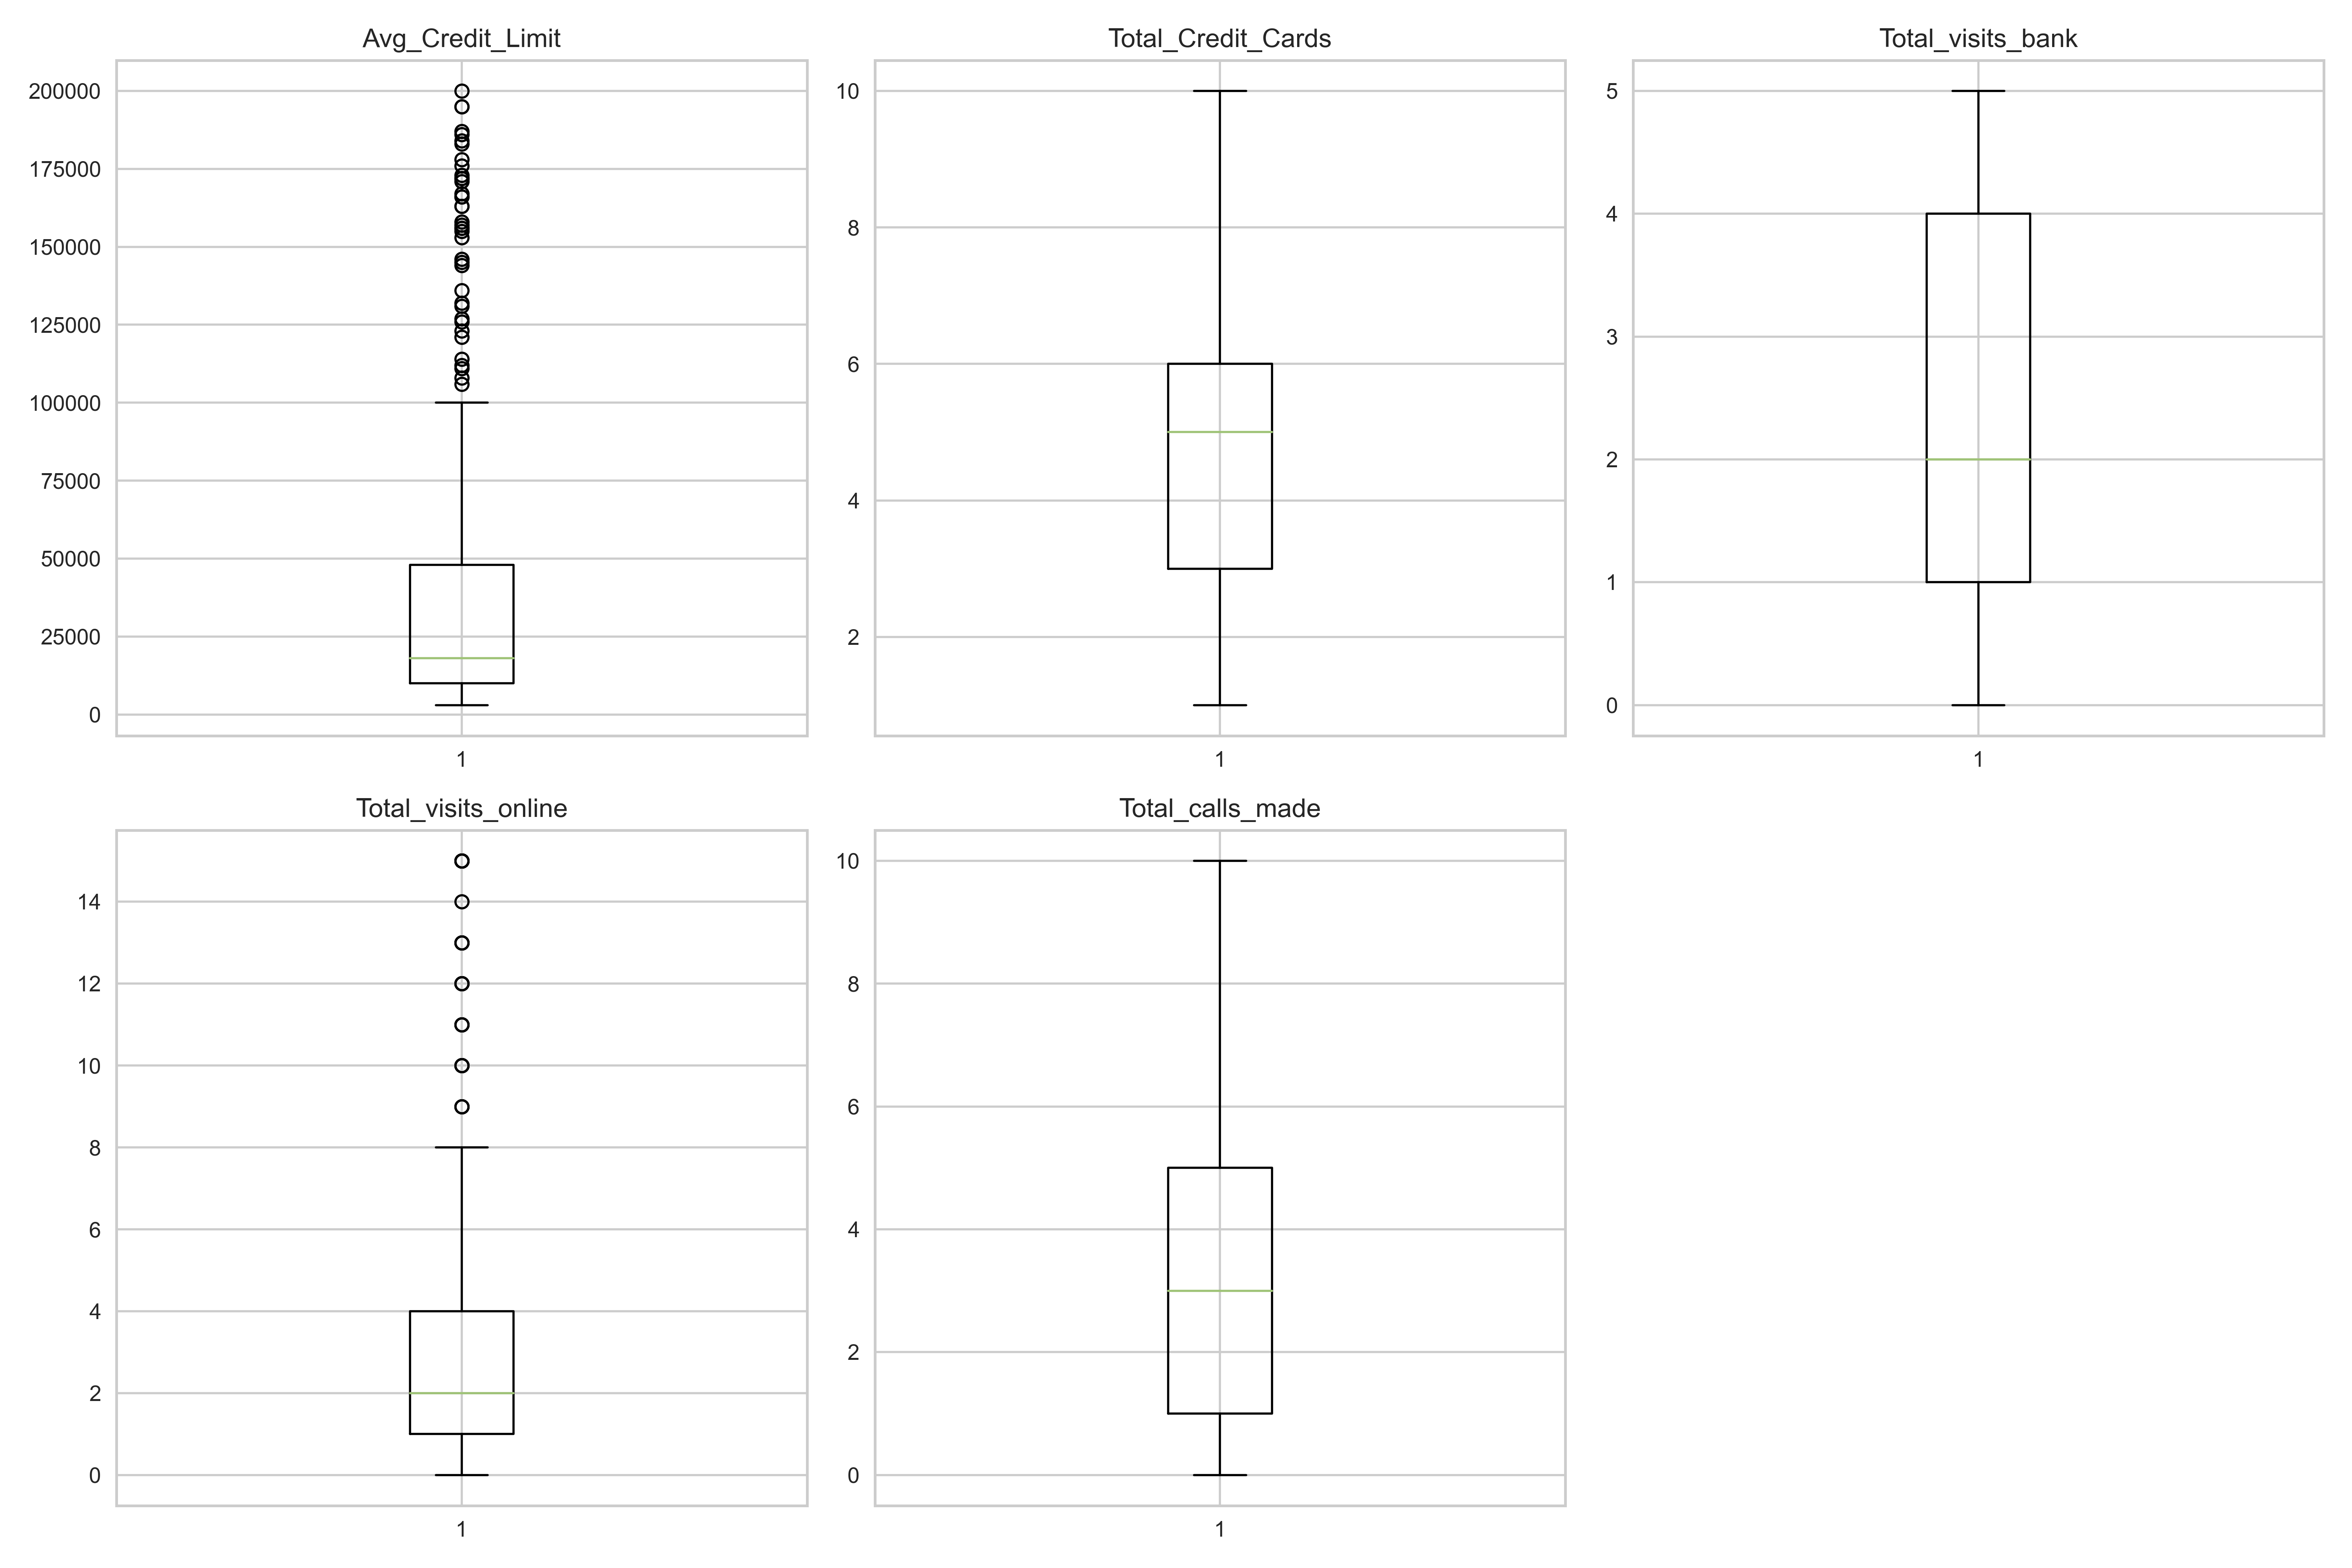
\includegraphics[width=\linewidth]{outlier.png}
			\caption{Plot for outlier detection}
			\label{fig:outlier}
		\end{figure}
		\begin{figure}[h]
			\centering
			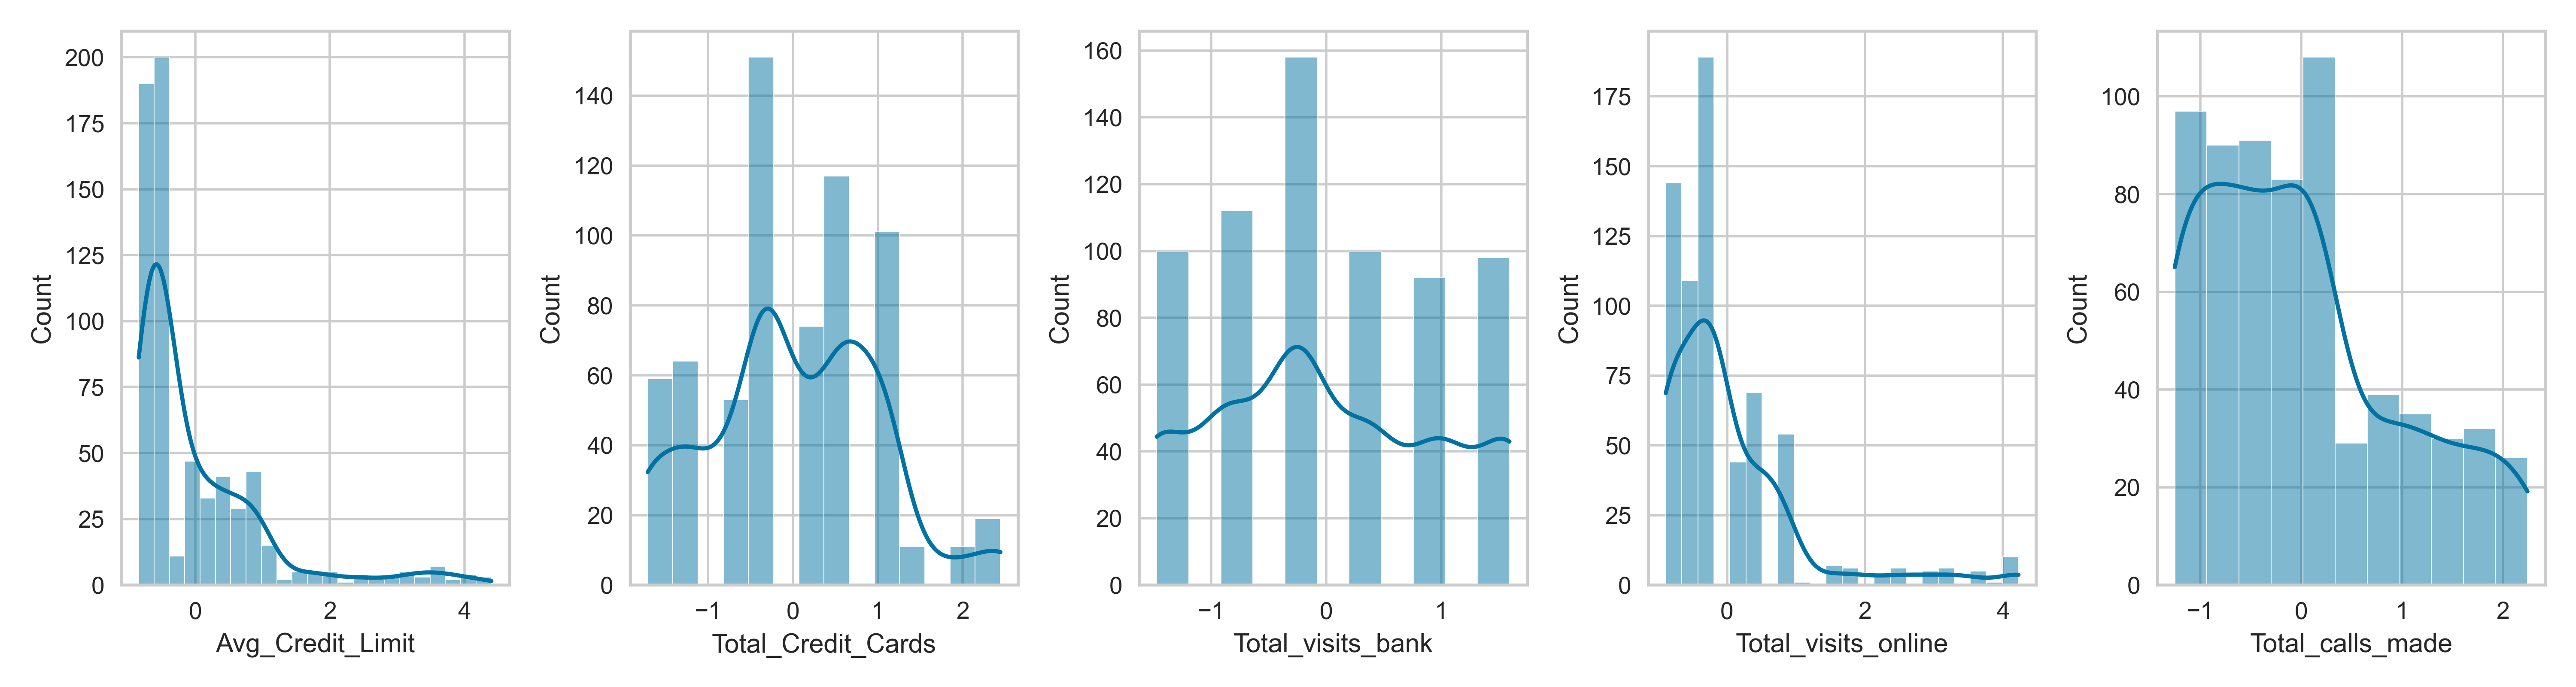
\includegraphics[width=\textwidth]{scaled_data.png}
			\caption{scaled data}
			\label{fig:scaled_data}
		\end{figure}
	%\clearpage
	\newpage
%%%%%%%%%%%%%%%%%%%%%%%%%%%%%%%%%%%%%%%%%%%%%%%%%%%%%%%%%%%%%%%%%%%%%%%%%%%%%%%%%
	\section{K-means Clustering}
		K-Means clustering is a popular unsupervised machine learning algorithm used to partition a dataset into distinct groups or clusters. The goal is to divide the data points into k clusters, where each data point belongs to the cluster with the nearest mean. The steps involved are as follows : 
		\begin{itemize}
			\item Initialization: Choose the number of clusters k and randomly initialize k centroids.
			
			\item Assignment: Assign each data point to the nearest centroid based on the Euclidean distance.
			
			\item Update: Recalculate the centroids as the mean of all data points assigned to each cluster.
			
			\item Repeat: Repeat the assignment and update steps until the centroids no longer change significantly or a maximum number of iterations is reached.
		\end{itemize}
		
		\begin{figure}[h]
			\centering
			\begin{subfigure}[t]{0.49\textwidth}
				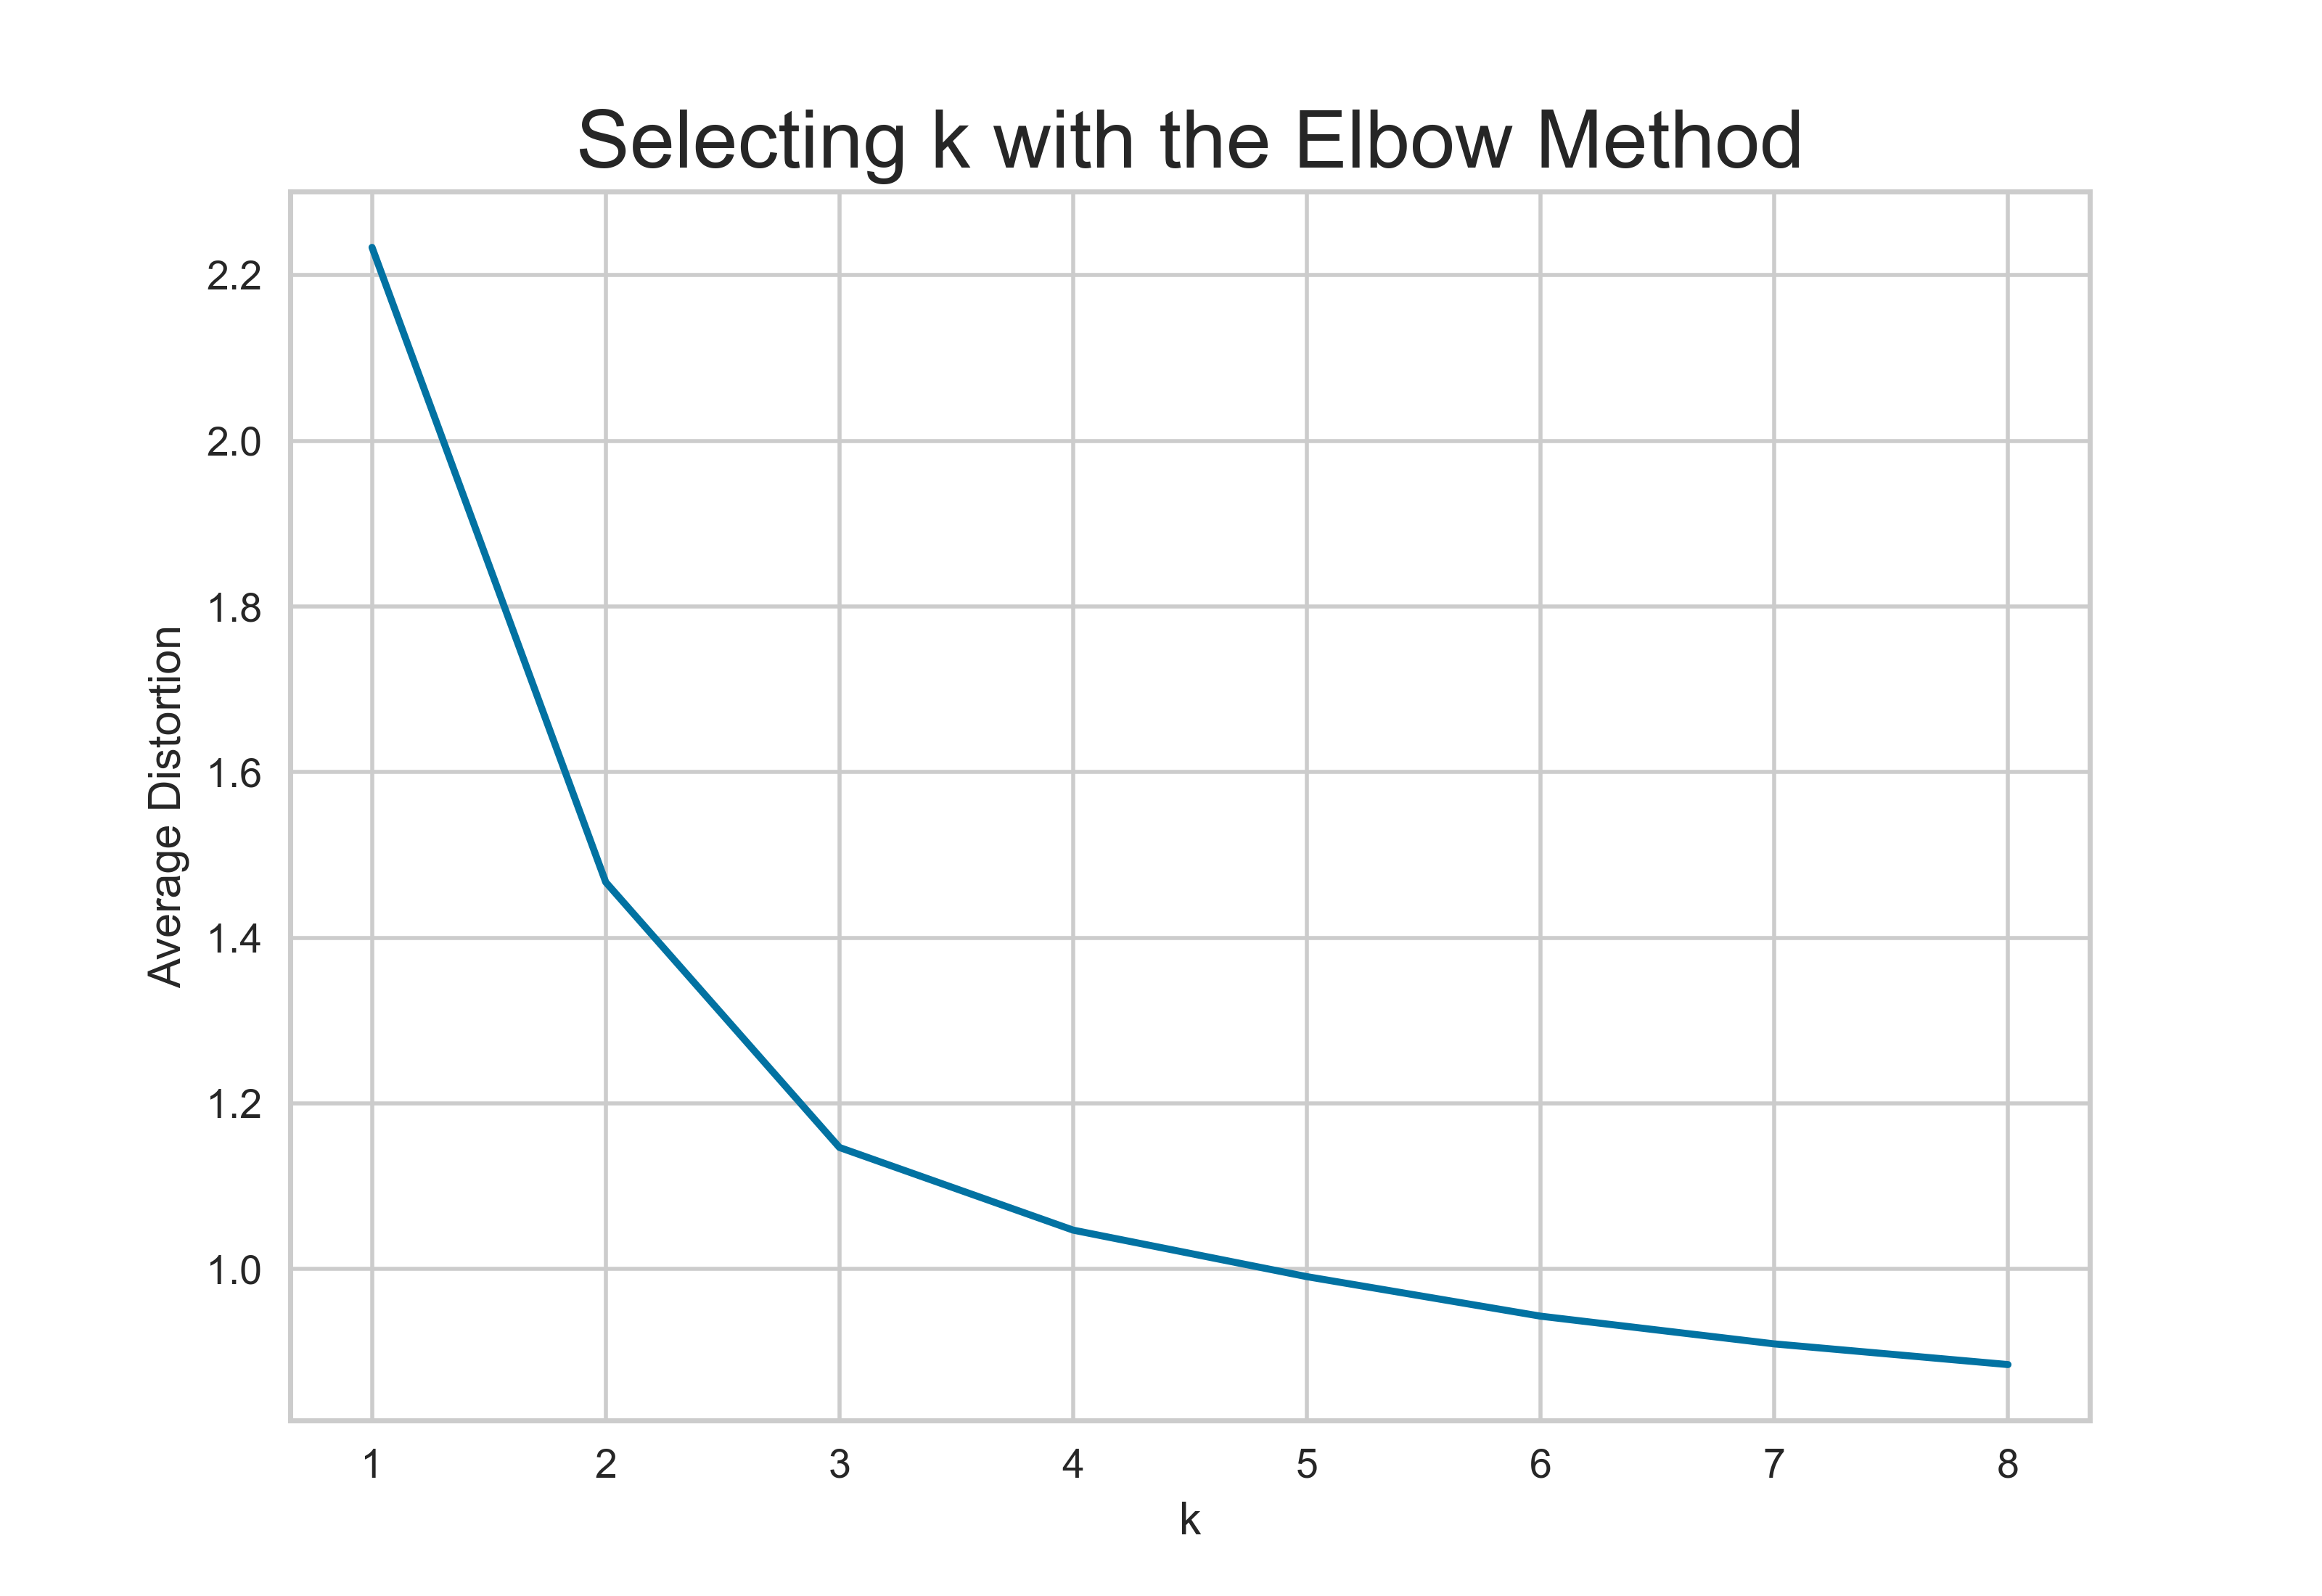
\includegraphics[width=\textwidth]{elbow.png}
				\caption{Average distortion across K to find elbow point.}
				\label{fig:elbow}
			\end{subfigure}
			\hfill
			\begin{subfigure}[t]{0.49\textwidth}
				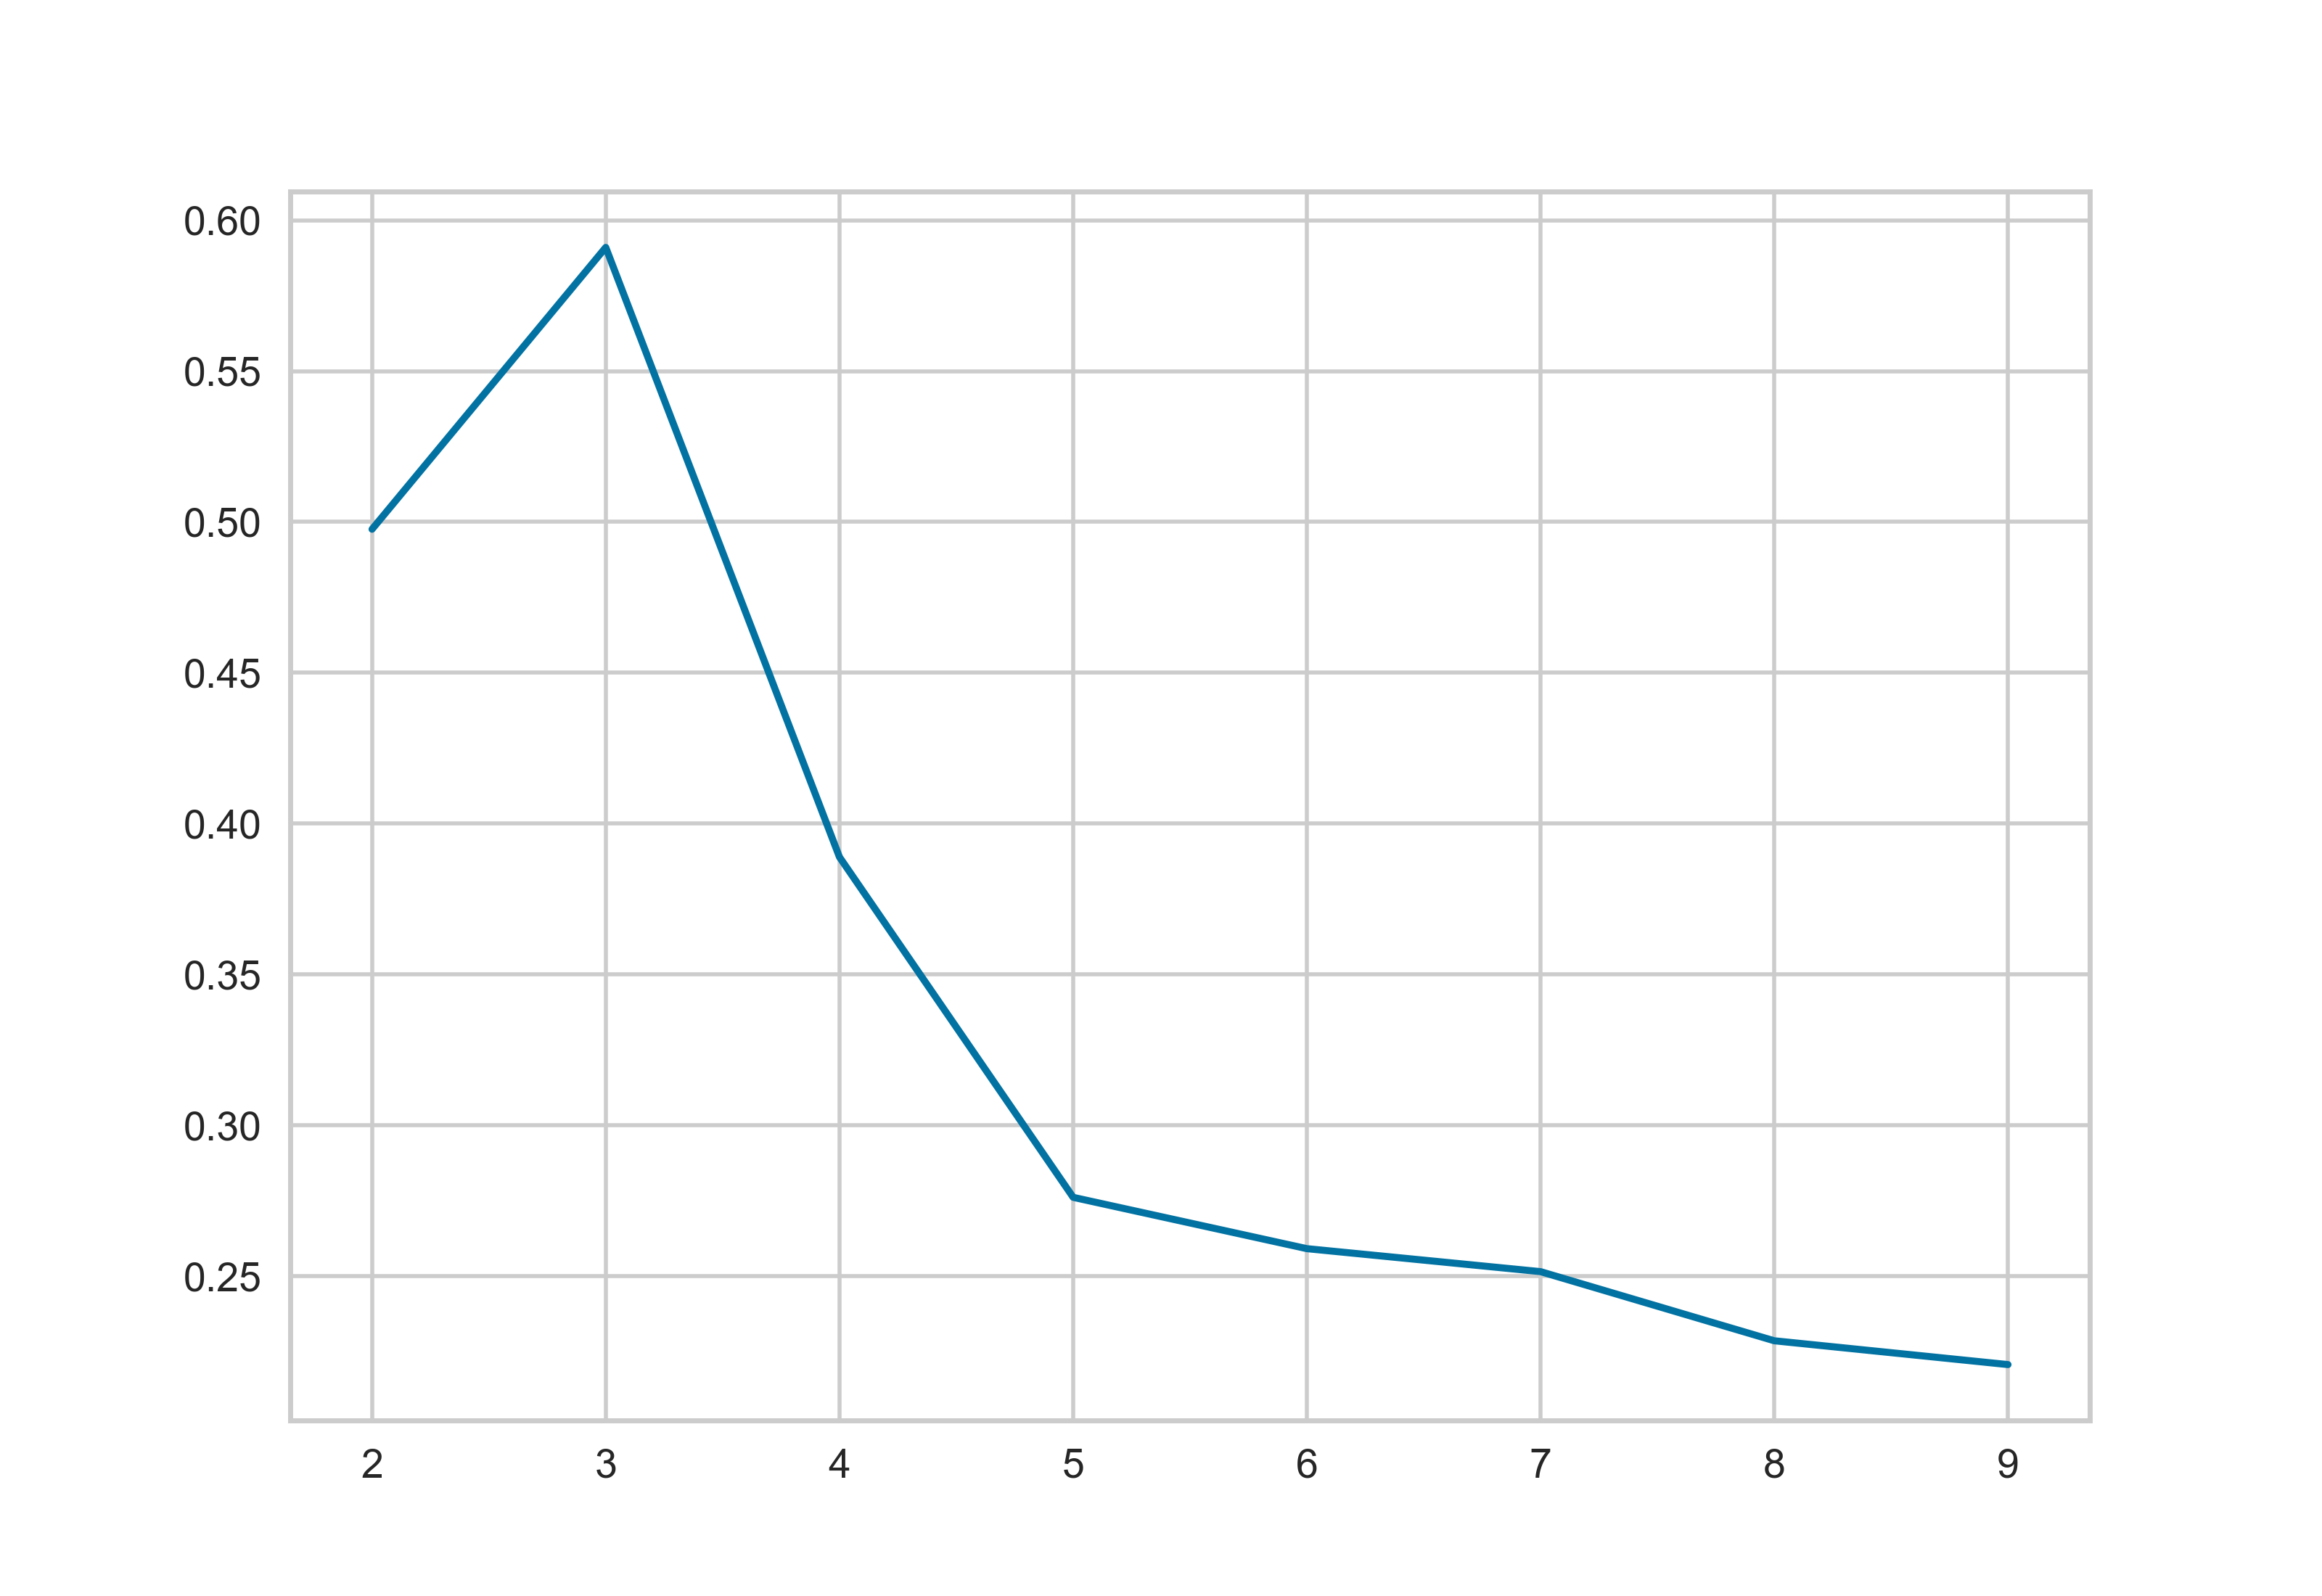
\includegraphics[width=\textwidth]{sil_score.png}
				\caption{Silhouette score with K}
				\label{fig:sil_score}
			\end{subfigure}
			\caption{Average distortion and Silhouette score across K. }
			\label{fig:Average distortion and Silhouette score across K.}
		\end{figure}	
		
		The metric used here for the KMeans distance is Euclidean. To figure out suitable K for the given data set I checked the Elbow method and Silhouette score for different K. The Plot of the sum of squared distances from each point to its assigned centroid (within-cluster sum of squares) for different values of k is shown in figure \ref{fig:elbow}. The optimal k is often found at the "elbow" point where the rate of decrease slows down. we observe that K =3. Also along side we calculate the silhouette score for different K as shown in figure \ref{fig:sil_score} and \ref{fig:Average distortion and Silhouette score across K.}. Silhouette score measures how similar a data point is to its own cluster compared to other clusters. A higher silhouette score indicates better-defined clusters. From this analysis  we find that the optimal k for this data set is 3. The Silhouette score is highest for k = 3 : 0.59. we chose the final KMeans model with 3 clusters.
		\begin{figure}[h]
			\centering
			\begin{subfigure}[t]{0.49\textwidth}
				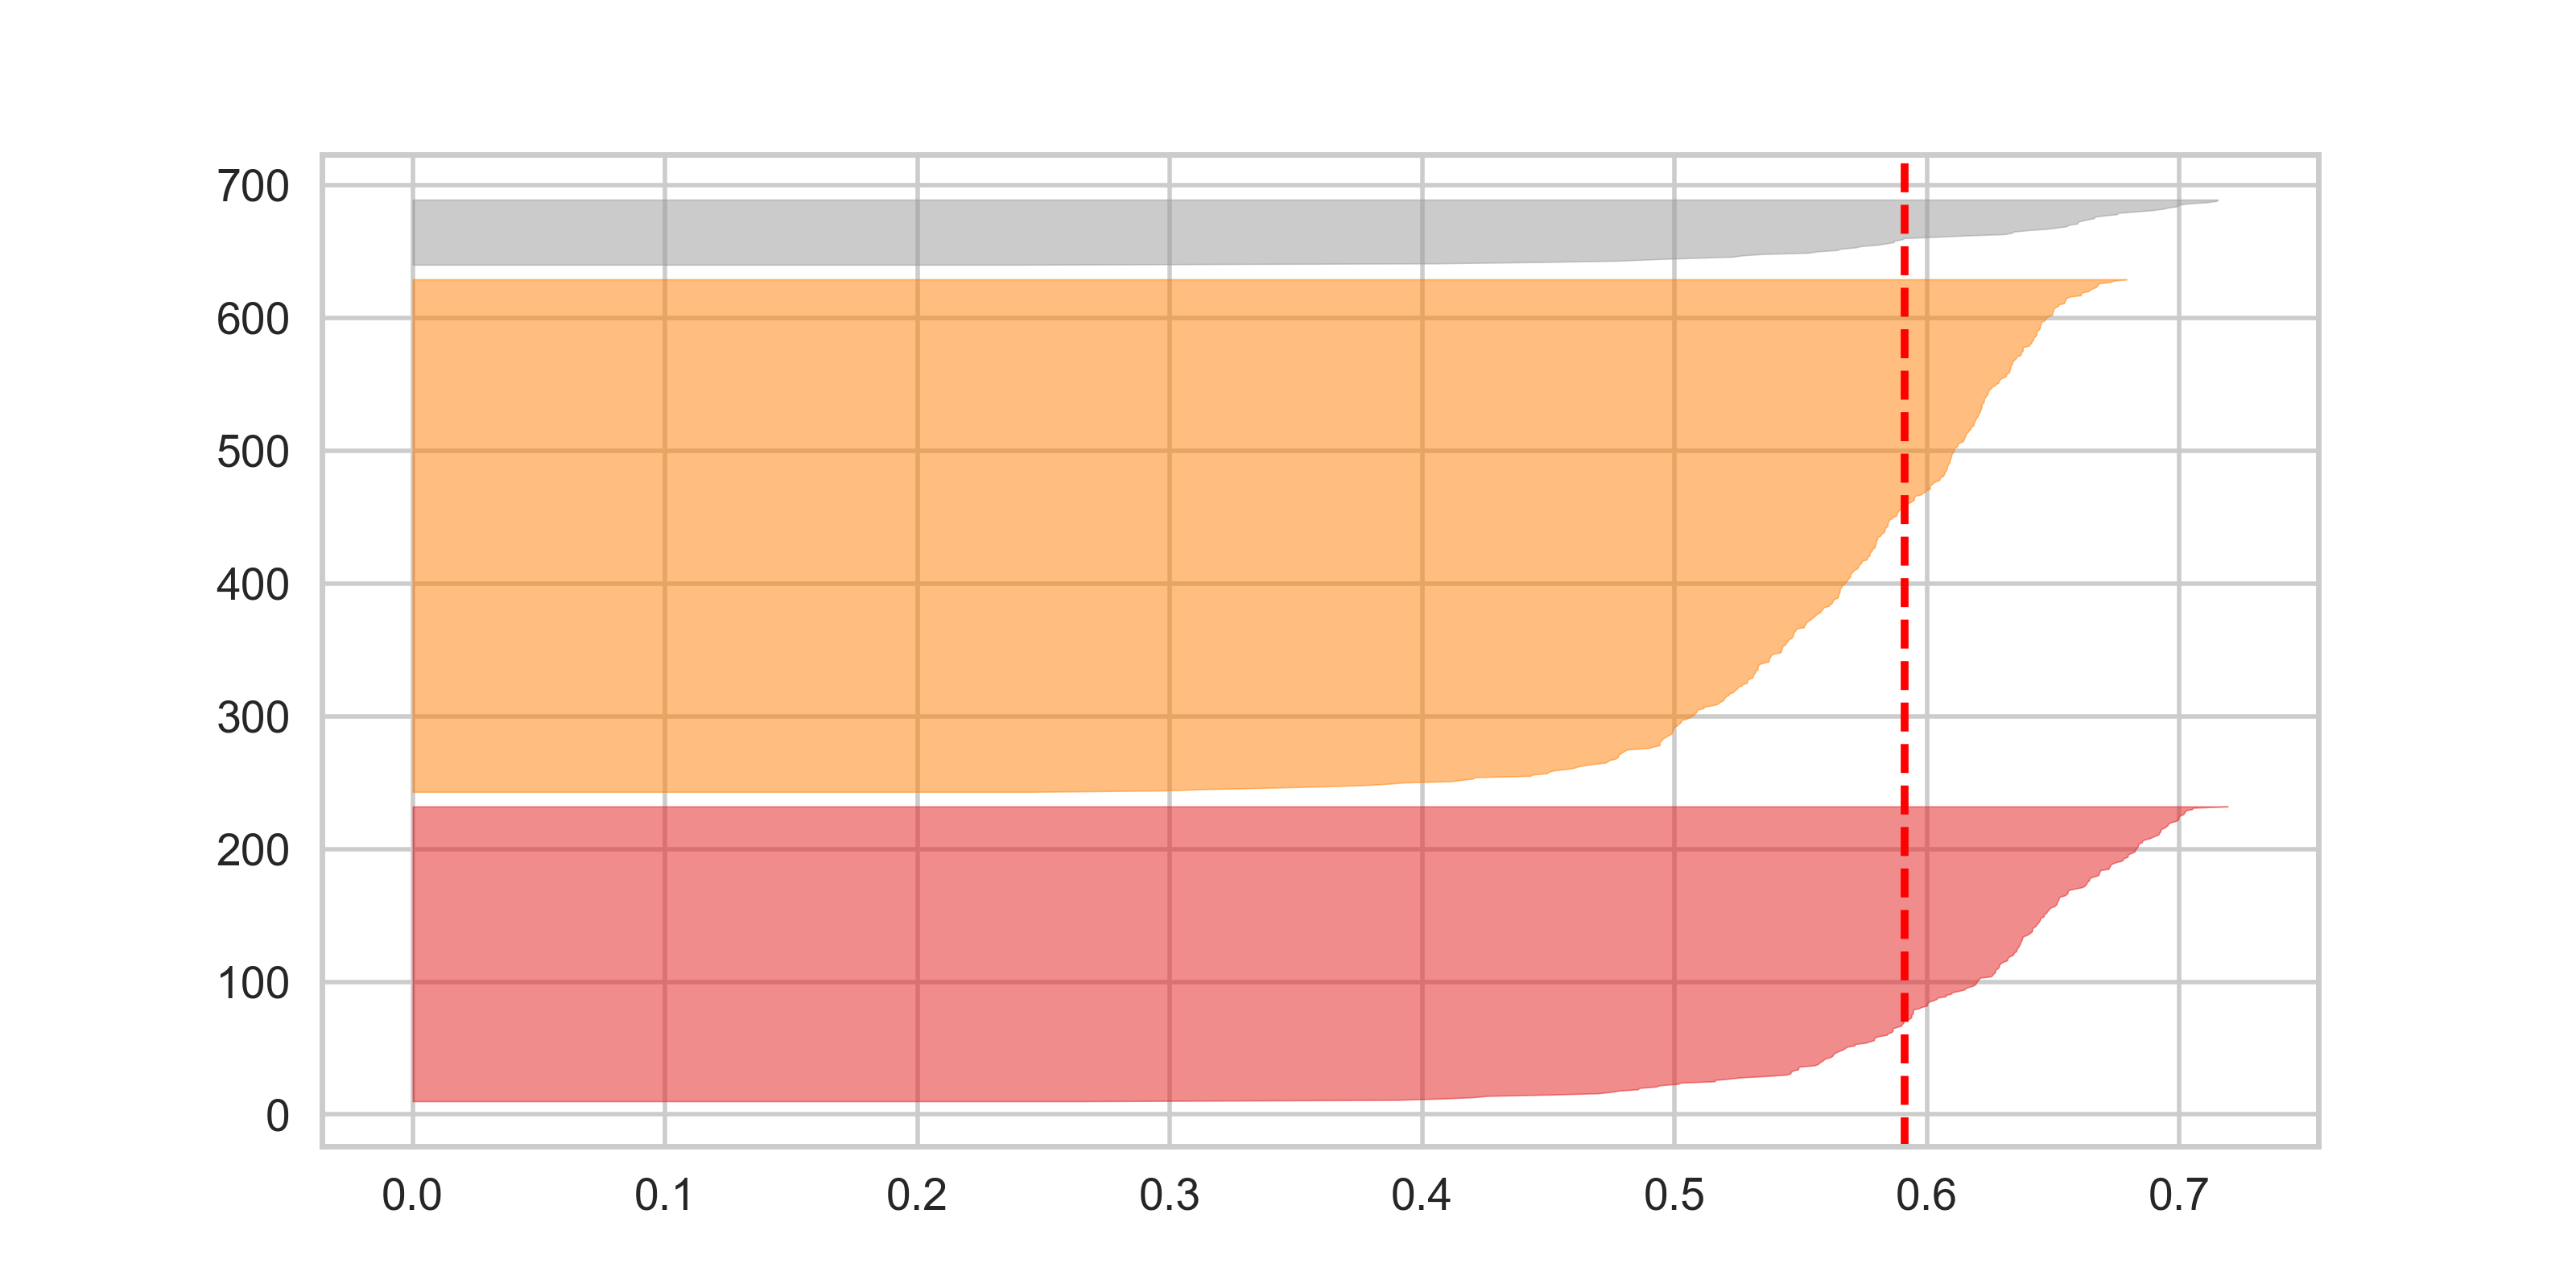
\includegraphics[width=\textwidth]{silhoute_K_3.png}
				\caption{Silhouette plot of KMeans Clustering for 660 samples in 3 centers.}
				\label{fig:silhoute_K_3.png}
			\end{subfigure}
			\hfill
			\begin{subfigure}[t]{0.49\textwidth}
				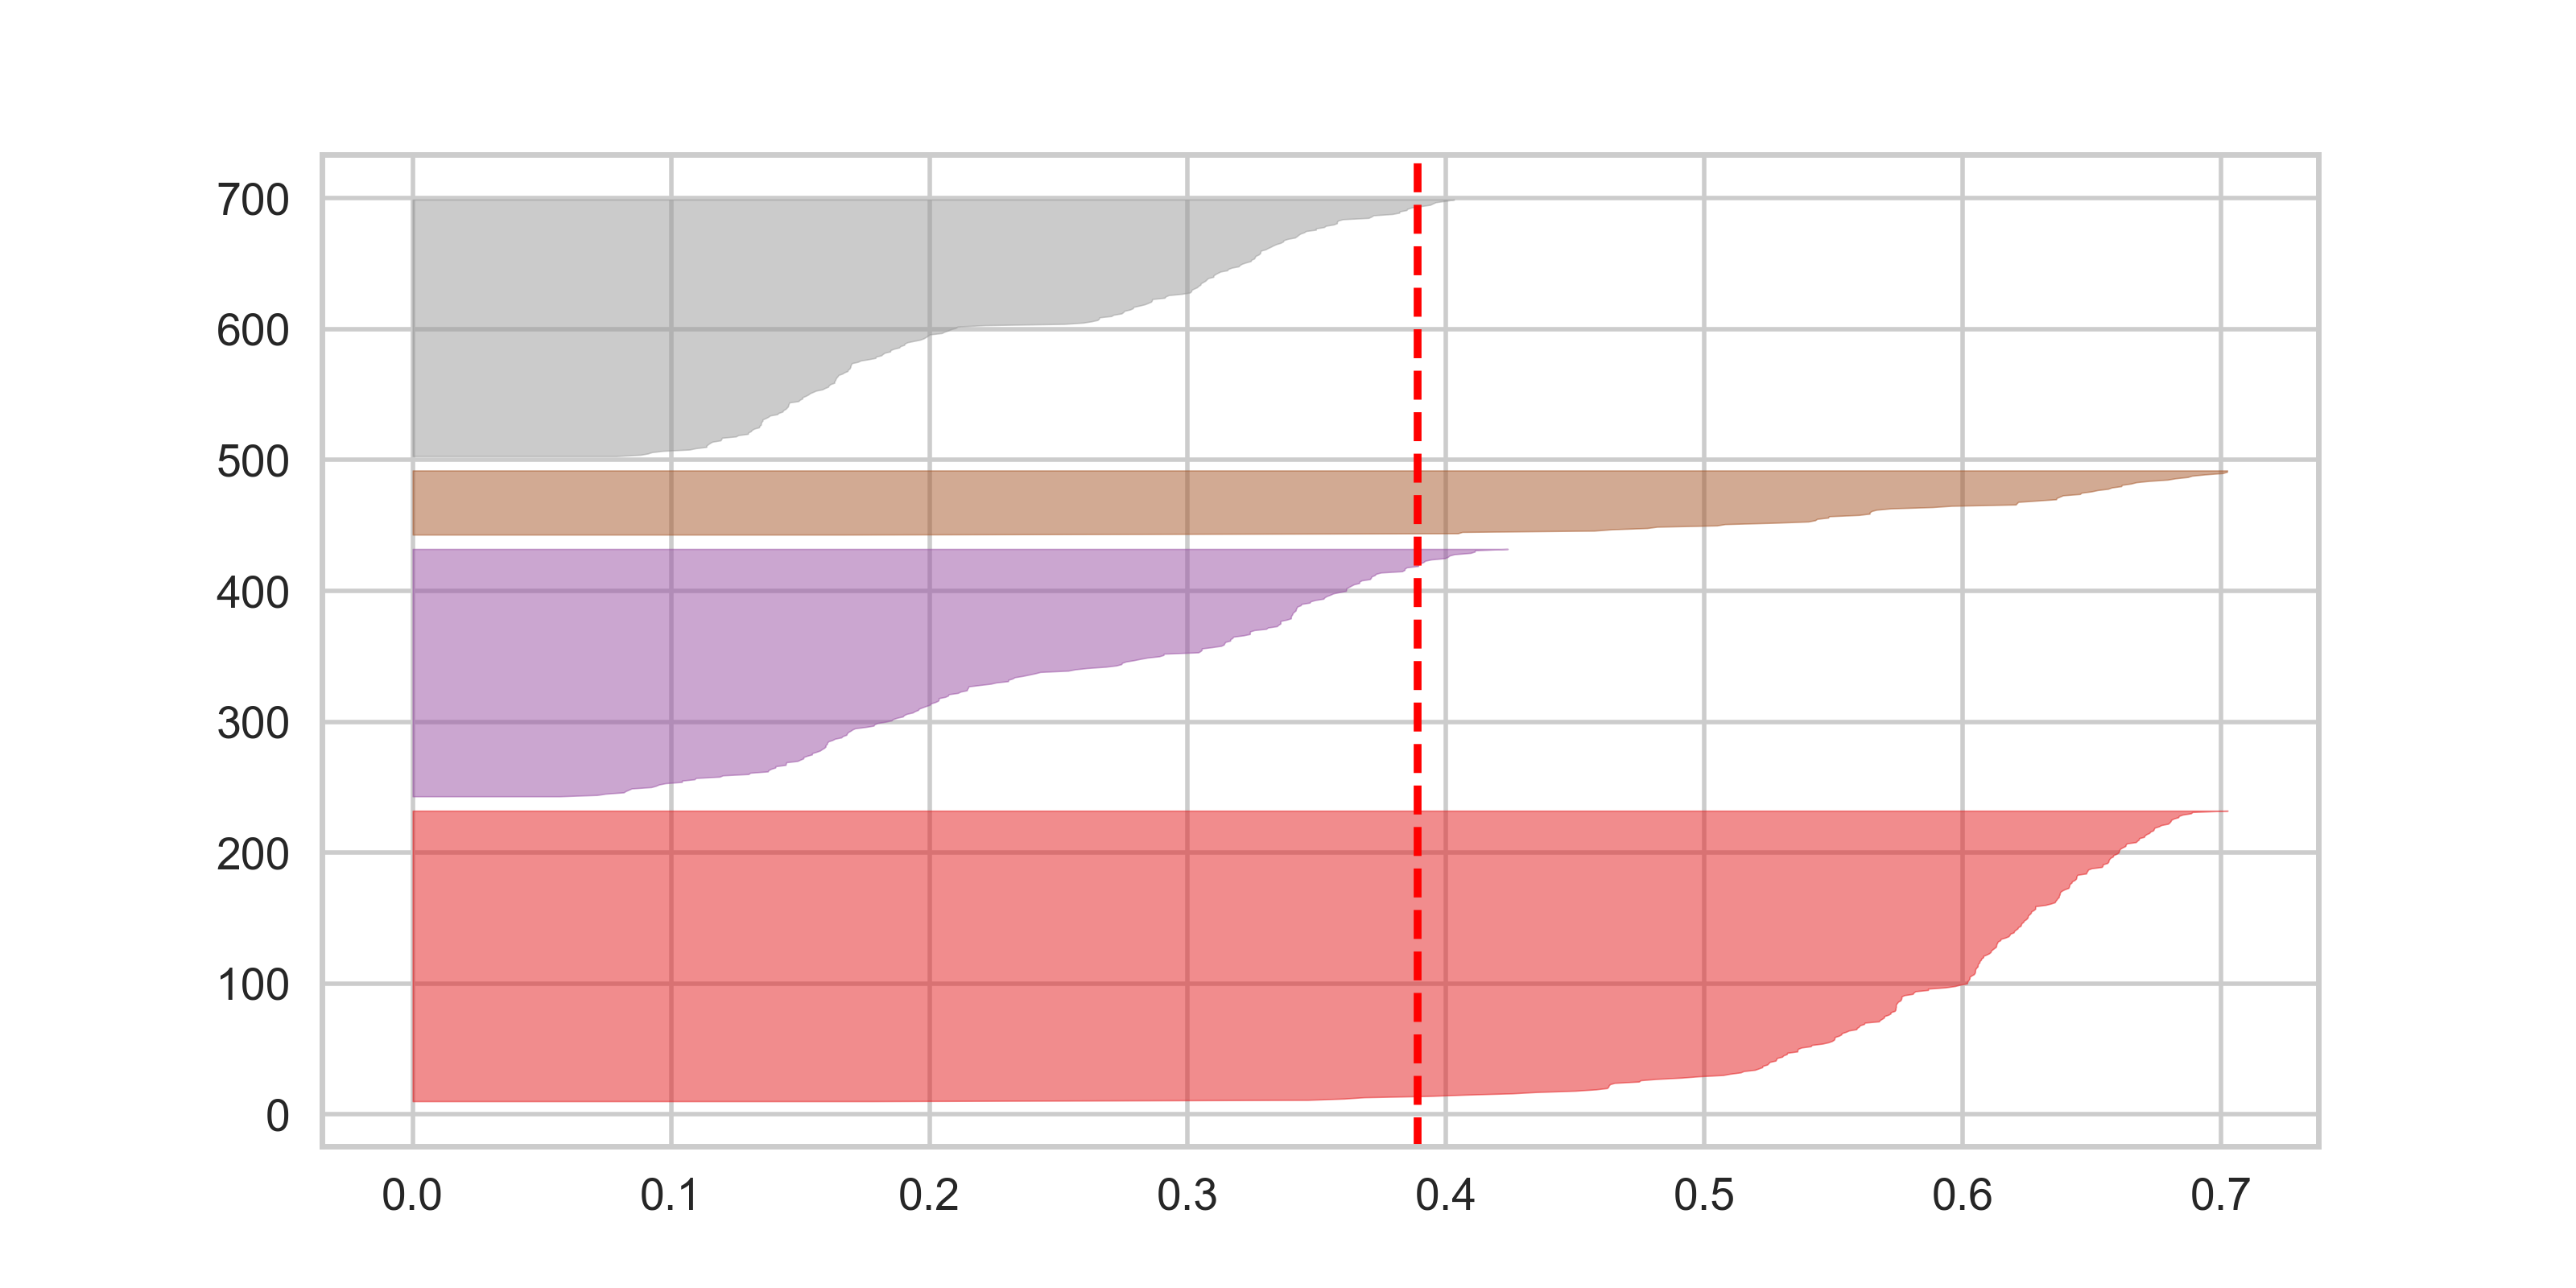
\includegraphics[width=\textwidth]{silhoute_K_4.png}
				\caption{Silhouette plot of KMeans Clustering for 660 samples in 4 centers.}
				\label{fig:silhoute_K_4.png}
			\end{subfigure}
			\begin{subfigure}[t]{0.49\textwidth}
				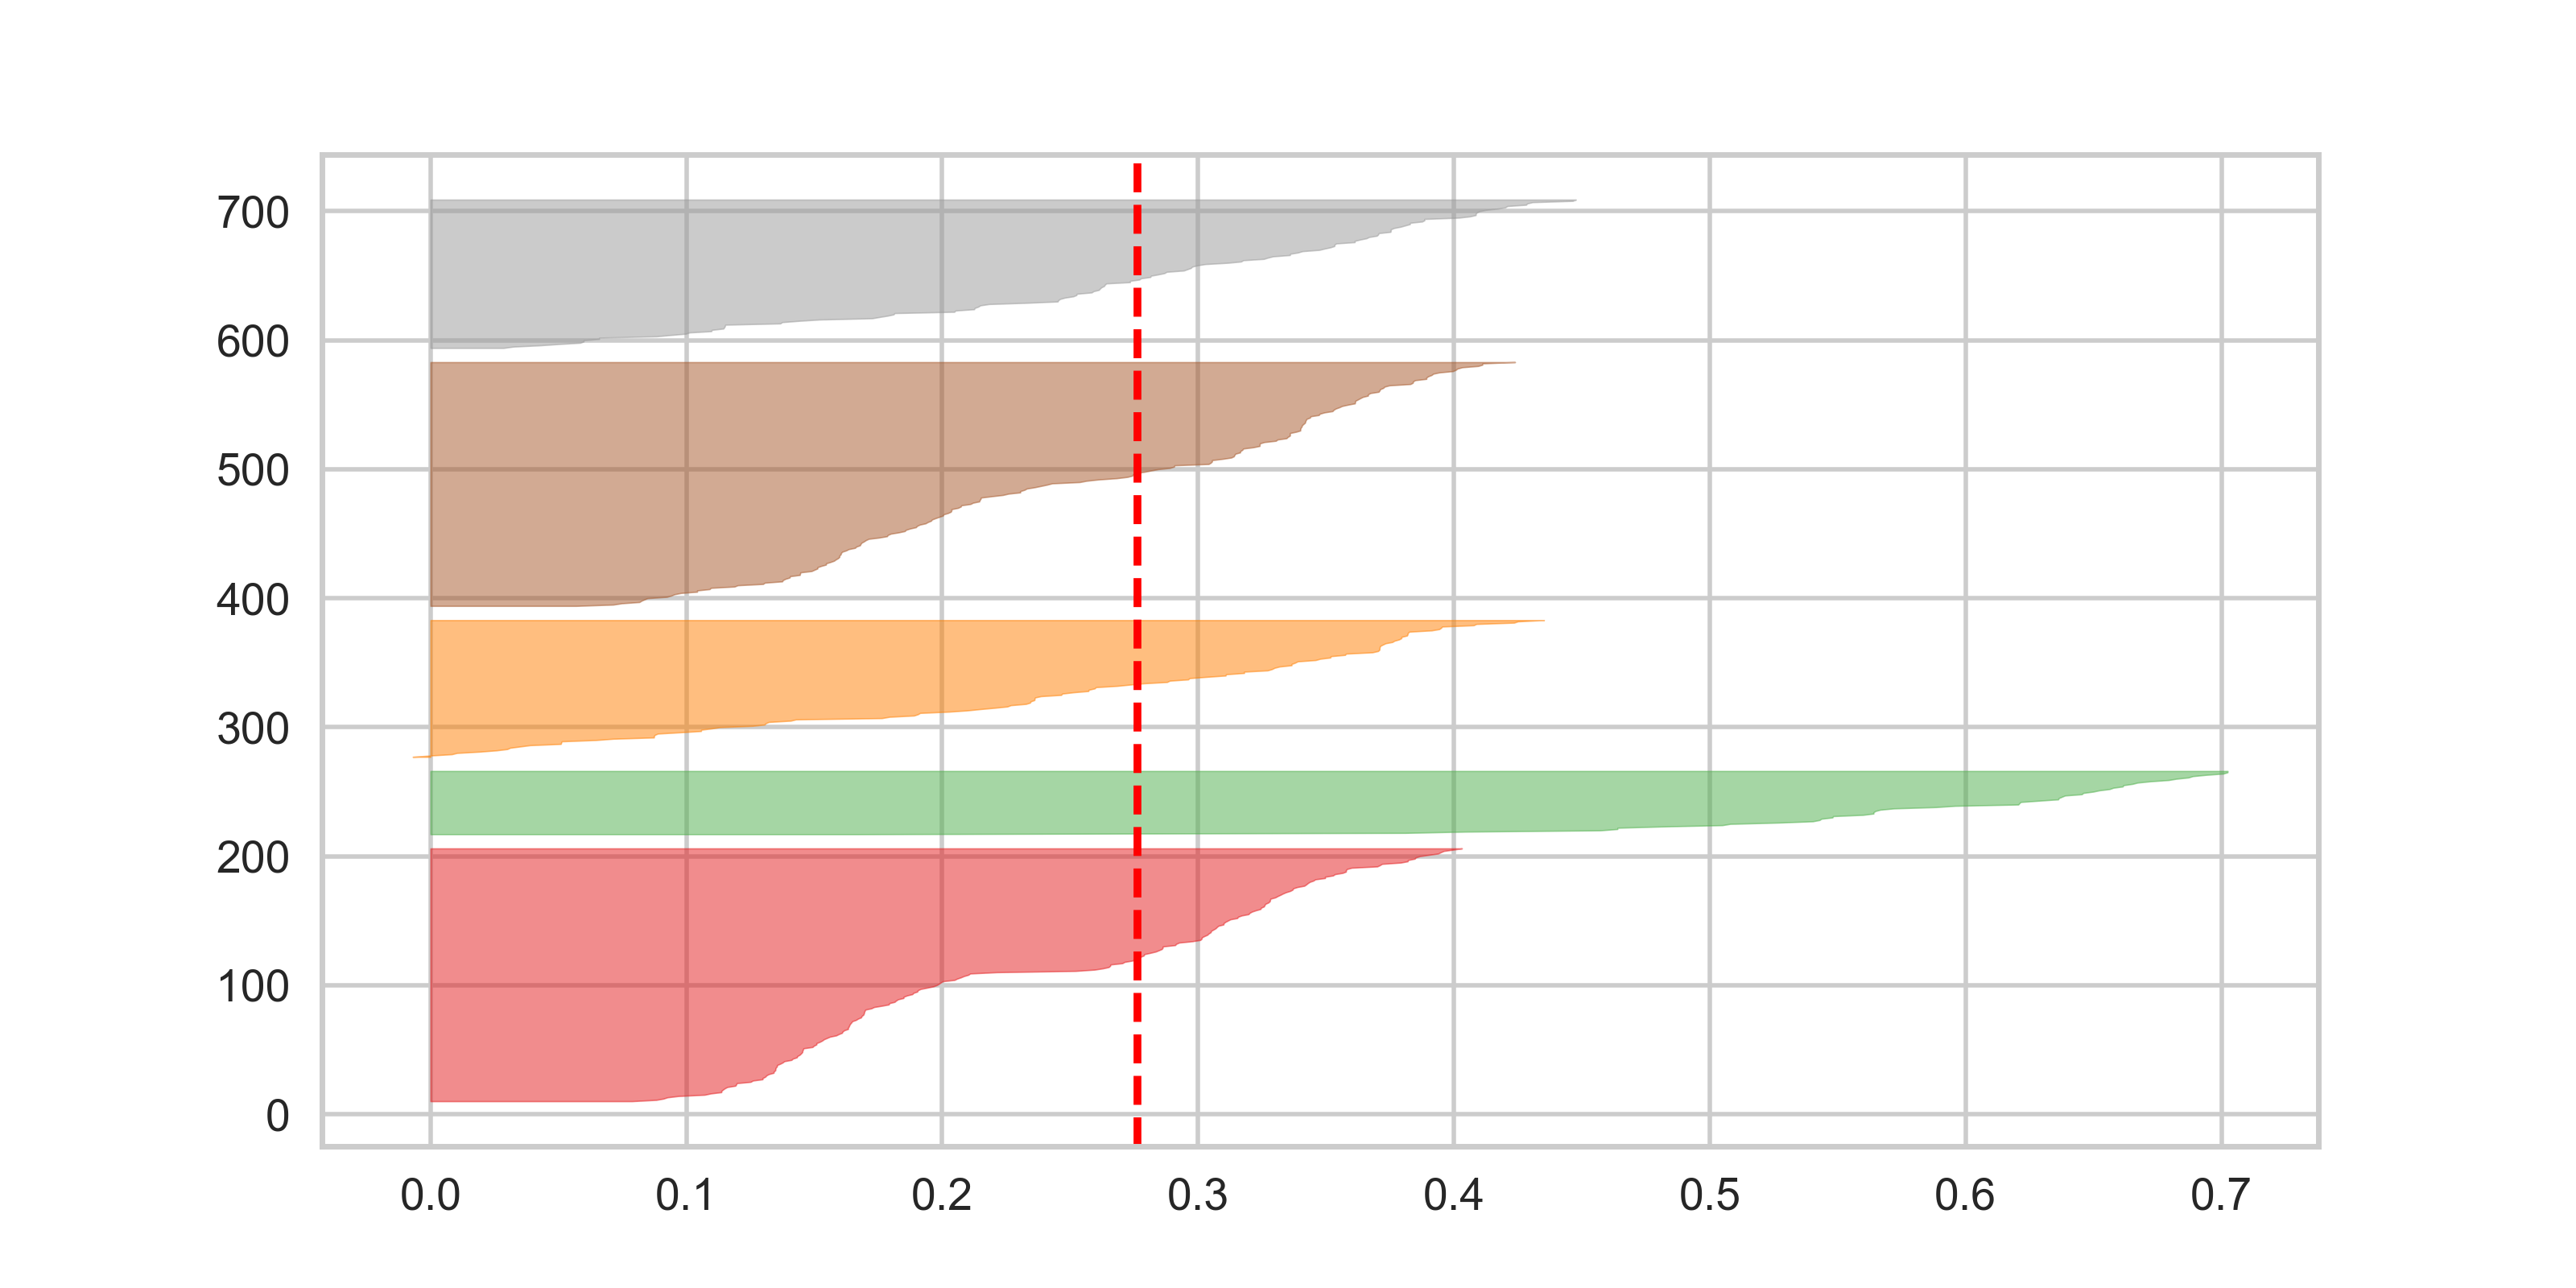
\includegraphics[width=\textwidth]{silhoute_K_5.png}
				\caption{Silhouette plot of KMeans Clustering for 660 samples in 5 centers.}
				\label{fig:silhoute_K_5.png}
			\end{subfigure}
			\hfill
			\begin{subfigure}[t]{0.49\textwidth}
				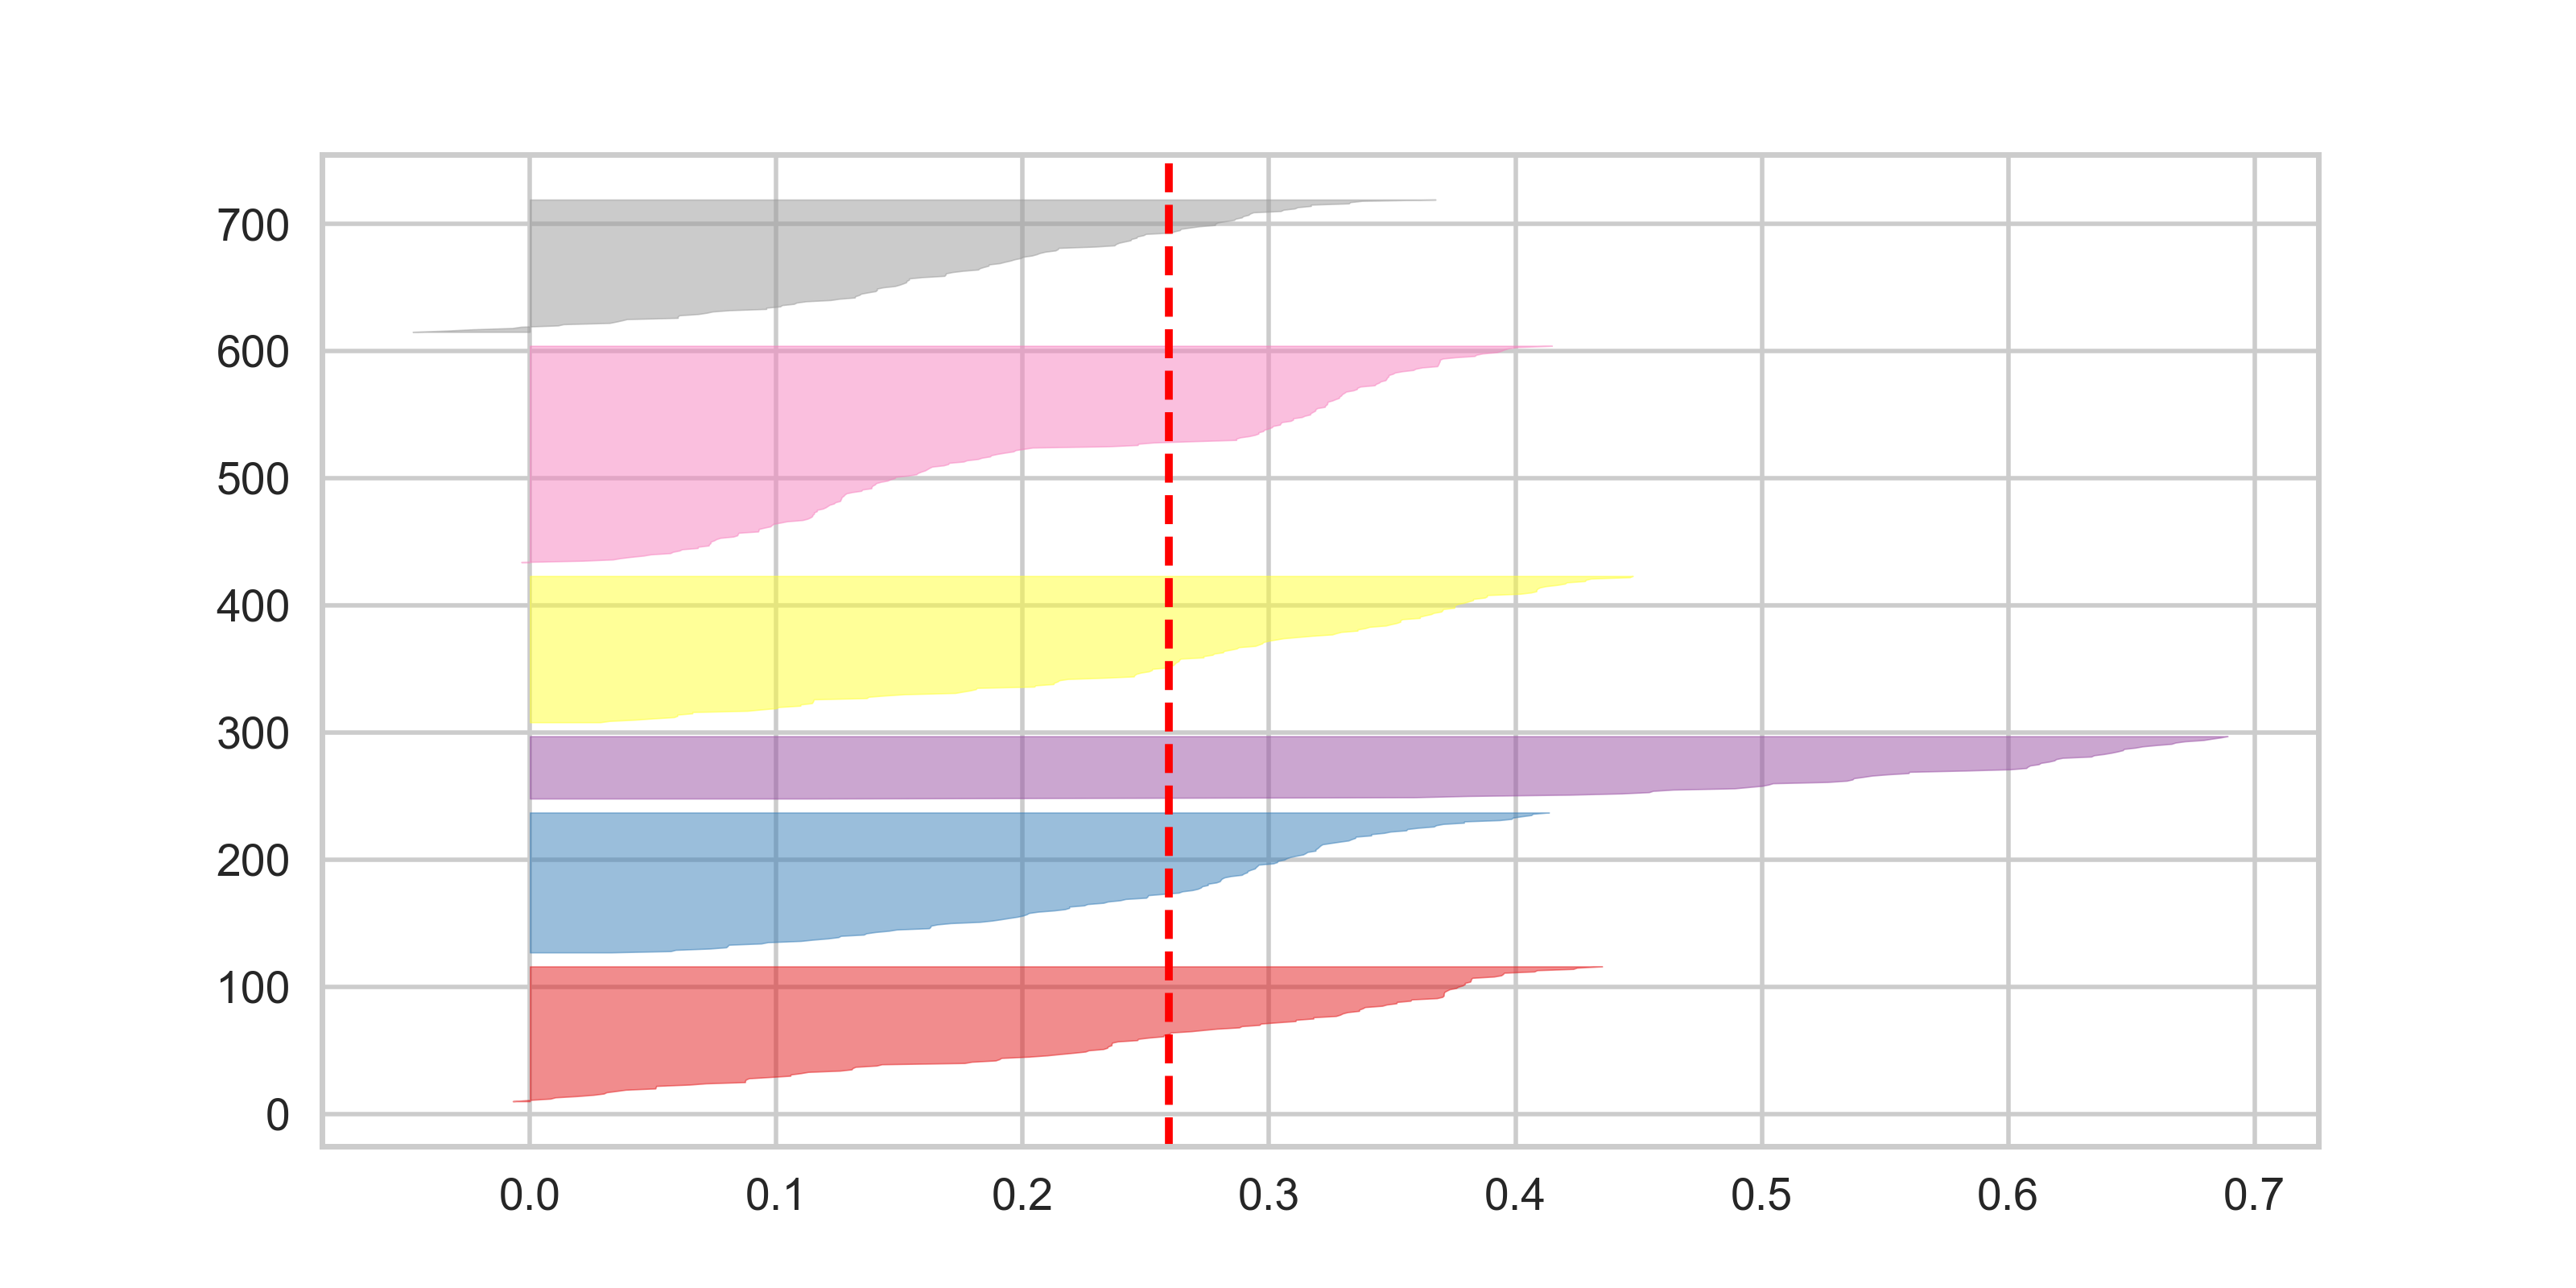
\includegraphics[width=\textwidth]{silhoute_K_6.png}
				\caption{Silhouette plot of KMeans Clustering for 660 samples in 6 centers.}
				\label{fig:silhoute_K_6.png}
			\end{subfigure}
			\caption{Silhouette Score visualization with varied K}
			\label{fig:Silhouette Score visualization iwith varied K}
		\end{figure}
		
		\begin{figure}[h]
			\centering
			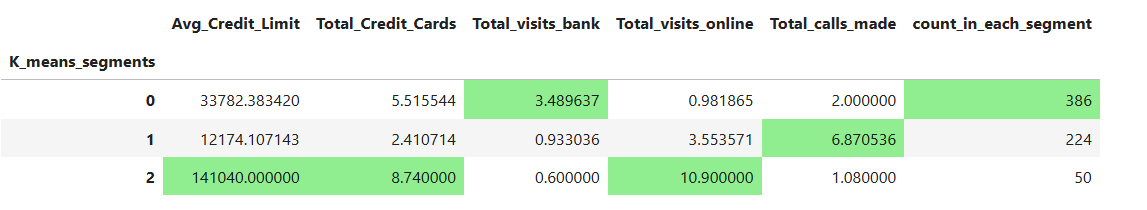
\includegraphics[width=\textwidth]{Kmeans_profile.png}
			\caption{Cluster profile from KMeans. K = 3}
			\label{fig:Kmeans_profile}
		\end{figure}
			Figure \ref{fig:Kmeans_profile} shows the cluster profile of 3 clusters obtained from the final KMeans model. It shows the mean values of each field corresponding to all three clusters. Figure \ref{fig:Kmeans_cluster_box_plots} shows box plot for all the numerical variables in each cluster categories.
		
		\begin{figure}[h]
			\centering
			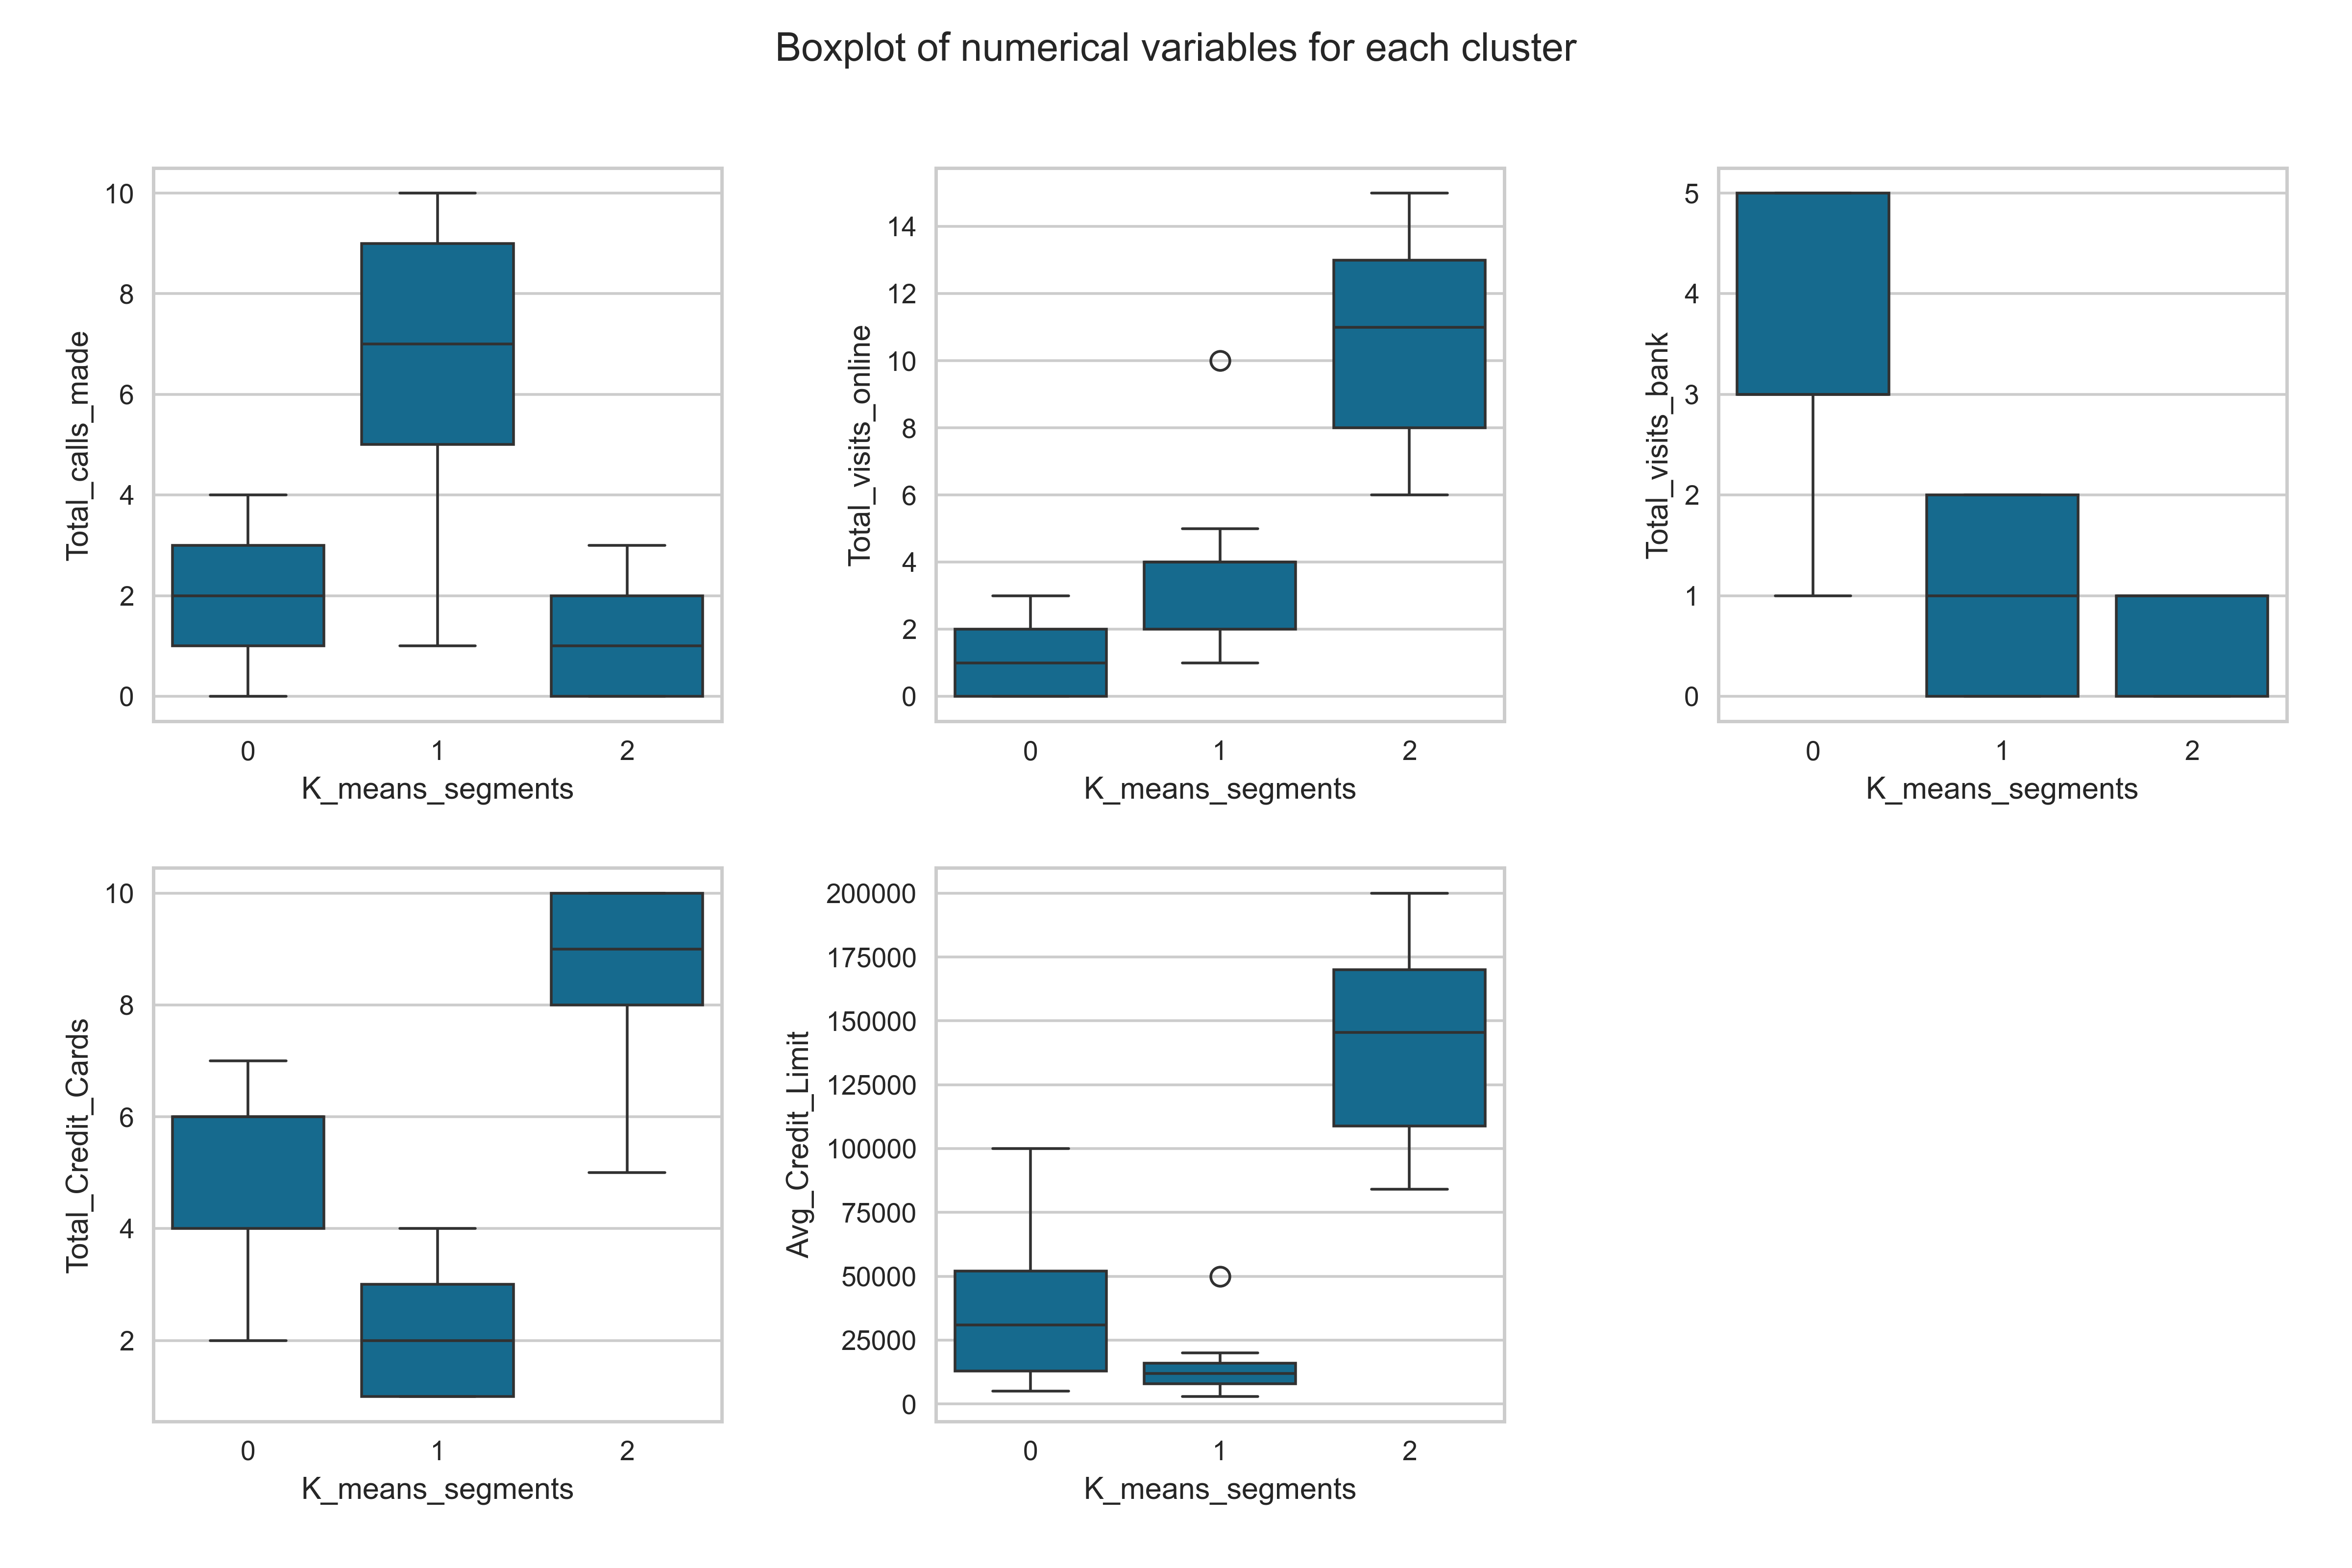
\includegraphics[width=\textwidth]{Kmeans_cluster_box_plots.png}
			\caption{Box plot of different clusters obtained from KMeans.}
			\label{fig:Kmeans_cluster_box_plots}
		\end{figure}
		From these two figures, \ref{fig:Kmeans_profile} and \ref{fig:Kmeans_cluster_box_plots} a summary for each cluster properties is generated.
		\begin{itemize}
			\item Cluster 0:
			\begin{itemize}
				\item There are 386 customers in this segment out of 660.
				\item 75\% of customers in this group made less than 3 calls.
				\item Atmost three online visits are made from these customers.
				\item These customers have relatively higher number of in person Bank visits than other two.
				\item 75 \% have 6 or less number of credit cards.
				\item Median credit limit is around 30,000. 
			\end{itemize}
			\item Cluster 1:
			\begin{itemize}
				\item There are 224 customers in this segment.
				\item This segment have made higher number of phone calls. At least half of them made more than 6 calls.
				\item 75 \% of them made less than 4 online visits.
				\item All of them had at most two visits to the bank in person.
				\item They have at most 4 credit cards.
				\item Median credit limit is very less around 12,000.
			\end{itemize}
			\item Cluster 2:
			\begin{itemize}
				\item There are only 50 customers in this segment out of 660.
				\item 75 \% of them made less than two phone calls.
				\item They made relatively a very high number of online visits.
				\item These customers don't visit to bank in person. At most they made 1 visit personally.
				\item They hold higher number of credit cards. Up to 10.
				\item Credit limit is also very high reaching up to 200,000.   
			\end{itemize}
			
		\end{itemize}
	
	\clearpage	
	\newpage
	\section{Hierarchical Clustering}
		Hierarchical clustering is a method of cluster analysis that seeks to build a hierarchy of clusters. It is particularly useful for identifying nested clusters and understanding the structure of the data. There are two main types of hierarchical clustering: 
		\begin{itemize}
			\item Agglomerative (Bottom-Up) Clustering: This approach starts with each data point as its own cluster and iteratively merges the closest pairs of clusters until all points are in a single cluster or a desired number of clusters is reached.
			\item Divisive (Top-Down) Clustering: This approach starts with all data points in a single cluster and iteratively splits the clusters into smaller clusters until each data point is its own cluster or a desired number of clusters is reached.
		\end{itemize}
		
		In this analysis, I have used Agglomerative Clustering approach. To figure out appropriate number of cluster for the data set I have used the dendrogram which is a tree-like diagram that shows the arrangement of the clusters produced by hierarchical clustering. Along side this I have calculated The Cophonetic correlation coefficients for various combination of metric and Linkage Methods. The cophenetic correlation coefficient measures how faithfully the dendrogram preserves the pairwise distances between the original data points. A higher cophenetic correlation indicates that the dendrogram accurately reflects the original data structure.
	
		\begin{figure}[h]
			\centering
			\begin{subfigure}[t]{0.49\textwidth}
				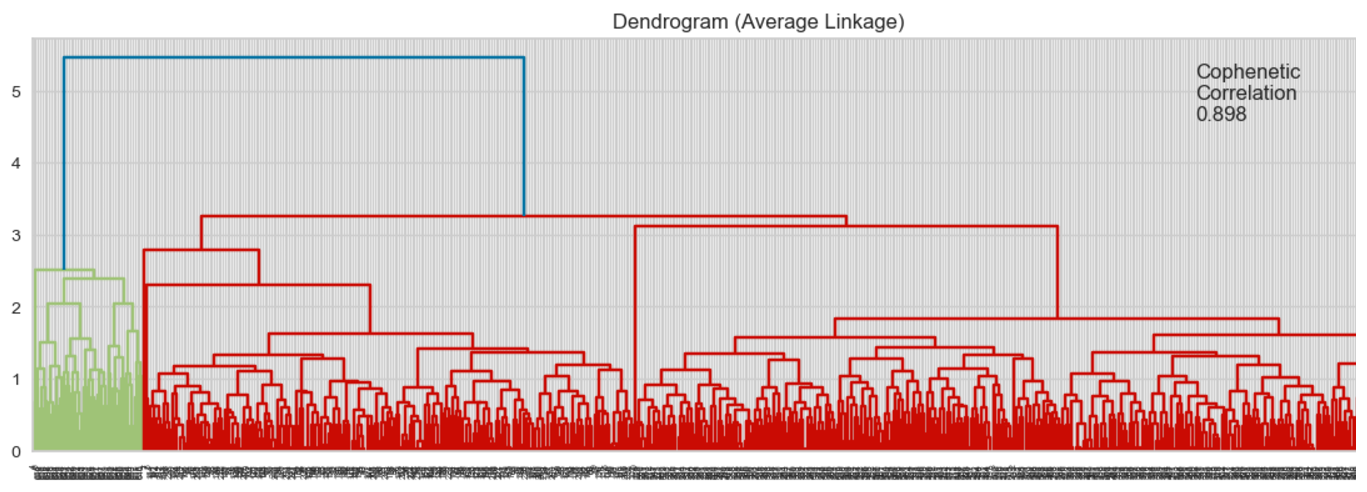
\includegraphics[width=\textwidth]{Euc_dendo_Average_linkage.png}
				\caption{Dendrogram for Average linkage. Cophenetic correlation = 0.898}
				\label{fig:Euc_dendo_Average_linkage.png}
			\end{subfigure}
			\hfill
			\begin{subfigure}[t]{0.49\textwidth}
				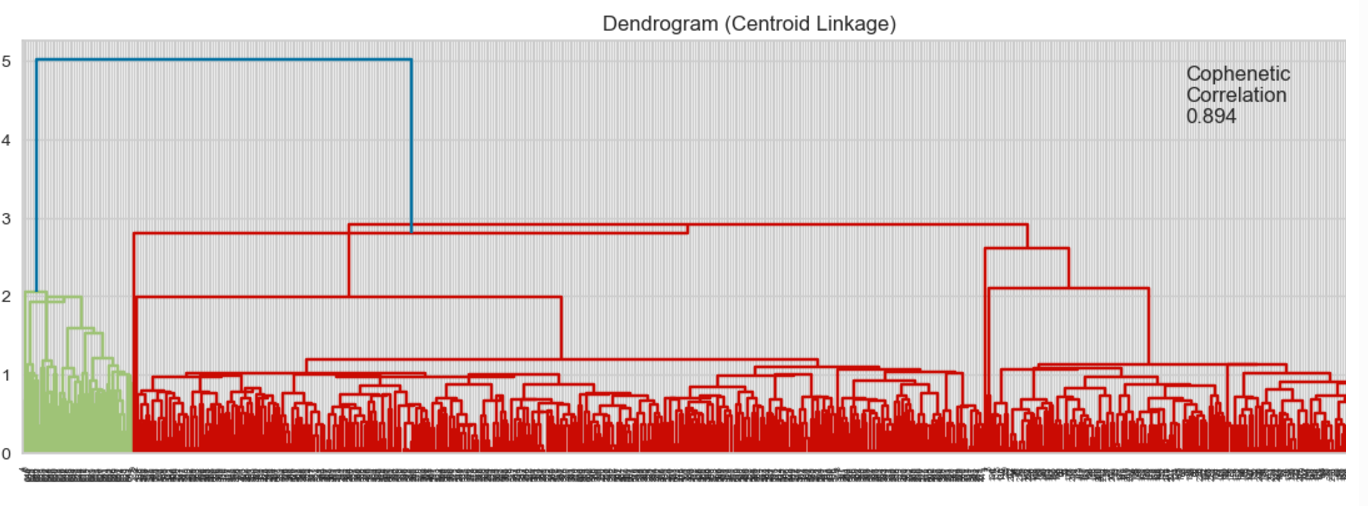
\includegraphics[width=\textwidth]{Euc_dendo_centroid_linkage.png}
				\caption{Dendrogram for centroid linkage. Cophenetic correlation = 0.894.}
				\label{fig:Euc_dendo_centroid_linkage.png}
			\end{subfigure}
			\begin{subfigure}[t]{0.49\textwidth}
				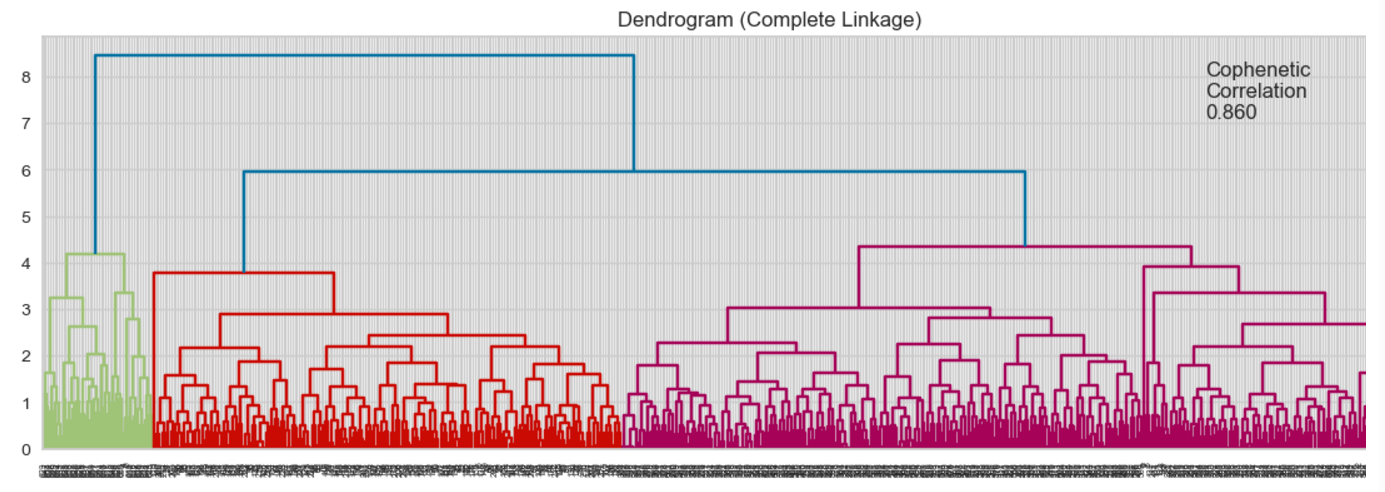
\includegraphics[width=\textwidth]{Euc_dendo_complete_linkage.png}
				\caption{Dendrogram for Complete linkage. Cophenetic correlation = 0.860 .}
				\label{fig:Euc_dendo_complete_linkage.pngg}
			\end{subfigure}
			\hfill
			\begin{subfigure}[t]{0.49\textwidth}
				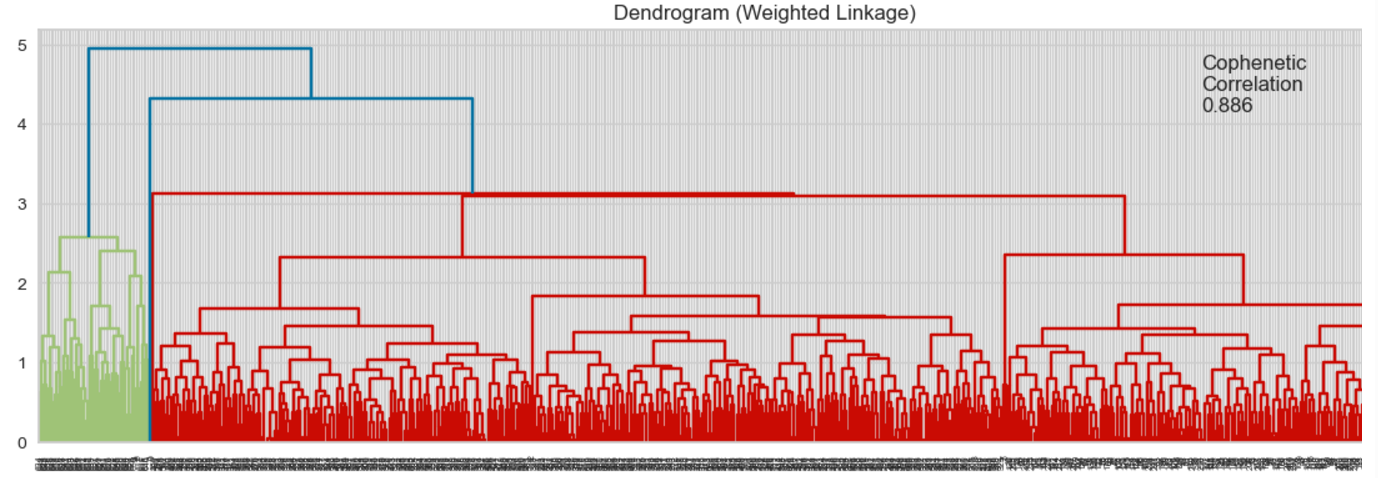
\includegraphics[width=\textwidth]{Euc_dendo_Weighted_linkage.png}
				\caption{Dendrogram for Weighted linkage. Cophenetic correlation = 0.886.}
				\label{fig:Euc_dendo_Weighted_linkage.png}
			\end{subfigure}
			\caption{Dendogram with different linkage methods for Euclidean metric.}
			\label{fig:Dendogram with different linkage methods for Euclidean metric.}
		\end{figure}
		I found that among different metric and linkage methods, Euclidean metric with Average linkage gave best correlation of 0.898. Figure \ref{fig:Dendogram with different linkage methods for Euclidean metric.} shows Dendrograms with different linkage methods for Euclidean metric with at least 0.8 of cophenetic correlation. From these reliable dendrograms it is observed that 3 clusters would have been appropriate for the dataset as beyond this the branches grew rapidly. So we chose the final Hierarchical(HC) model with 3 clusters. 
	
		\begin{figure}[h]
			\centering
			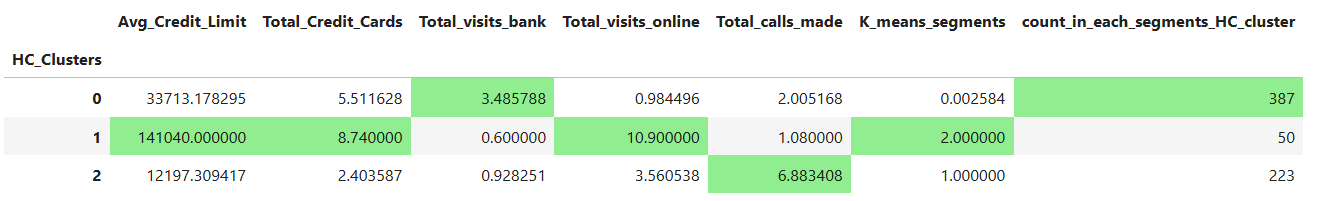
\includegraphics[width=\textwidth]{HC_profile.png}
			\caption{Cluster profile from Hierarchical clustering. No. of clusters = 3}
			\label{fig:HC_profile}
		\end{figure}
		Figure \ref{fig:HC_profile} shows the cluster profile of 3 clusters obtained from the final HC model. It shows the mean values of each field corresponding to all three clusters. Figure \ref{fig:HC_cluster_box_plots} shows box plot for all the numerical variables in each cluster categories.
		
		\begin{figure}[h]
			\centering
			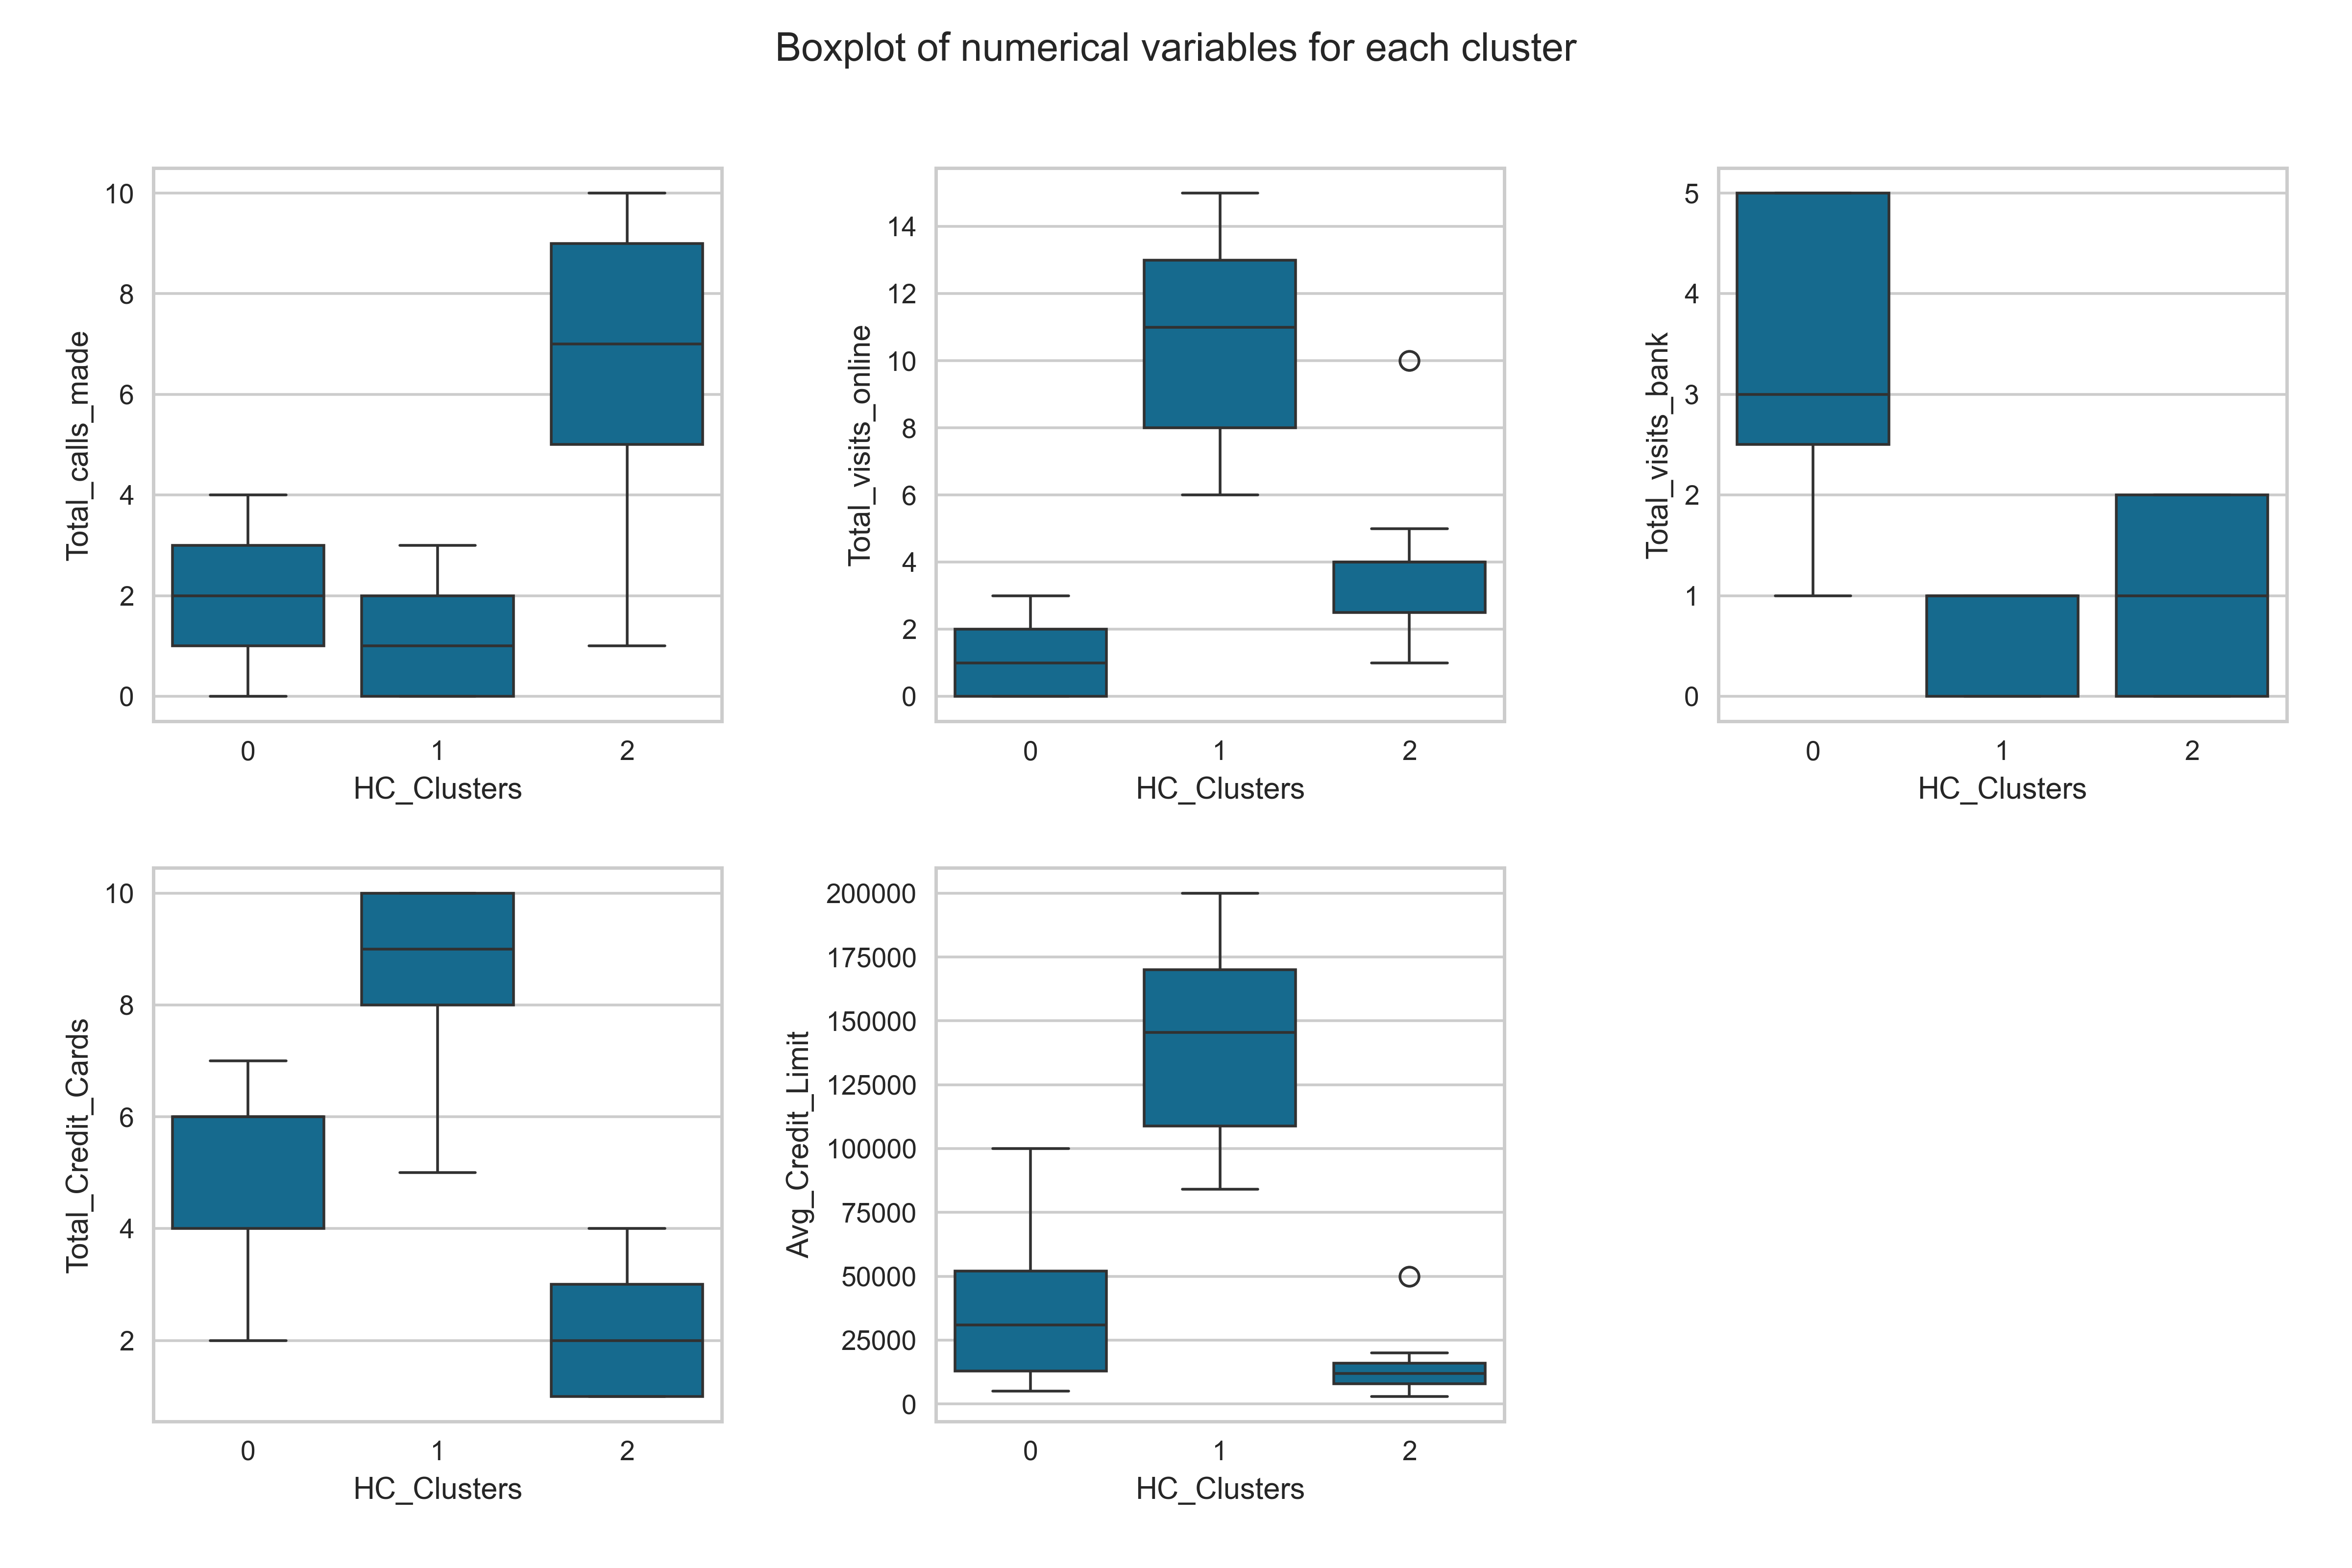
\includegraphics[width=\textwidth]{HC_cluster_box_plots.png}
			\caption{Box plot of different clusters obtained from Hierarchical clustering.}
			\label{fig:HC_cluster_box_plots}
		\end{figure}
		
		From these two figures, \ref{fig:HC_profile} and \ref{fig:HC_cluster_box_plots} a summary for each cluster properties is generated.
		\begin{itemize}
			\item Cluster 0:
			\begin{itemize}
				\item There are 387 customers in this segment out of 660.
				\item 75\% of customers in this group made less than 3 calls.
				\item At most three online visits are made from these customers.
				\item These customers have relatively higher number of in person Bank visits than other two.
				\item 75 \% have 6 or less number of credit cards.
				\item Median credit limit is around 30,000. 
			\end{itemize}
			\item Cluster 1:
			\begin{itemize}
				\item There are only 50 customers in this segment out of 660.
				\item 75 \% of them made less than two phone calls.
				\item They made relatively a very high number of online visits.
				\item These customers don't visit to bank in person. At most they made 1 visit personally.
				\item They hold higher number of credit cards. Up to 10.
				\item Credit limit is also very high reaching up to 200,000.   
			\end{itemize}
			\item Cluster 2:
			\begin{itemize}
				\item There are 223 customers in this segment.
				\item This segment have made higher number of phone calls. At least half of them made more than 6 calls.
				\item 75 \% of them made less than 4 online visits.
				\item All of them had at most two visits to the bank in person.
				\item They have atmost 4 credit cards.
				\item Median credit limit is very less around 12,000.
			\end{itemize}
			
		\end{itemize}
		
	
	\clearpage
	\newpage	
	\section{Comparison between two techniques}
	
		The results from both clustering techniques KMeans and Hierarchical(HC) are same both qualitatively and quantitatively. Both of them gave 3 clusters with almost exact identity/properties, only cluster 1 and 2 were interchanged. This can be observed from Figure \ref{fig:Cluster Method Comparision}. The bar plots are identical with cluster 1 and 2 interchanged. Also this is evident from cluster visualization with 2 features in figure \ref{fig:Cluster Visualization}, Only colors of cluster 1 and 2 are interchanged. The number of customers were also almost same for each segments in both methods.
		
		In terms of time complexity HC took significantly higher time than KMeans since HC is connectivity based clustering. It grows as O(n*n). 
	
		\begin{figure}[h]
			\centering
			\begin{subfigure}[t]{0.49\textwidth}
				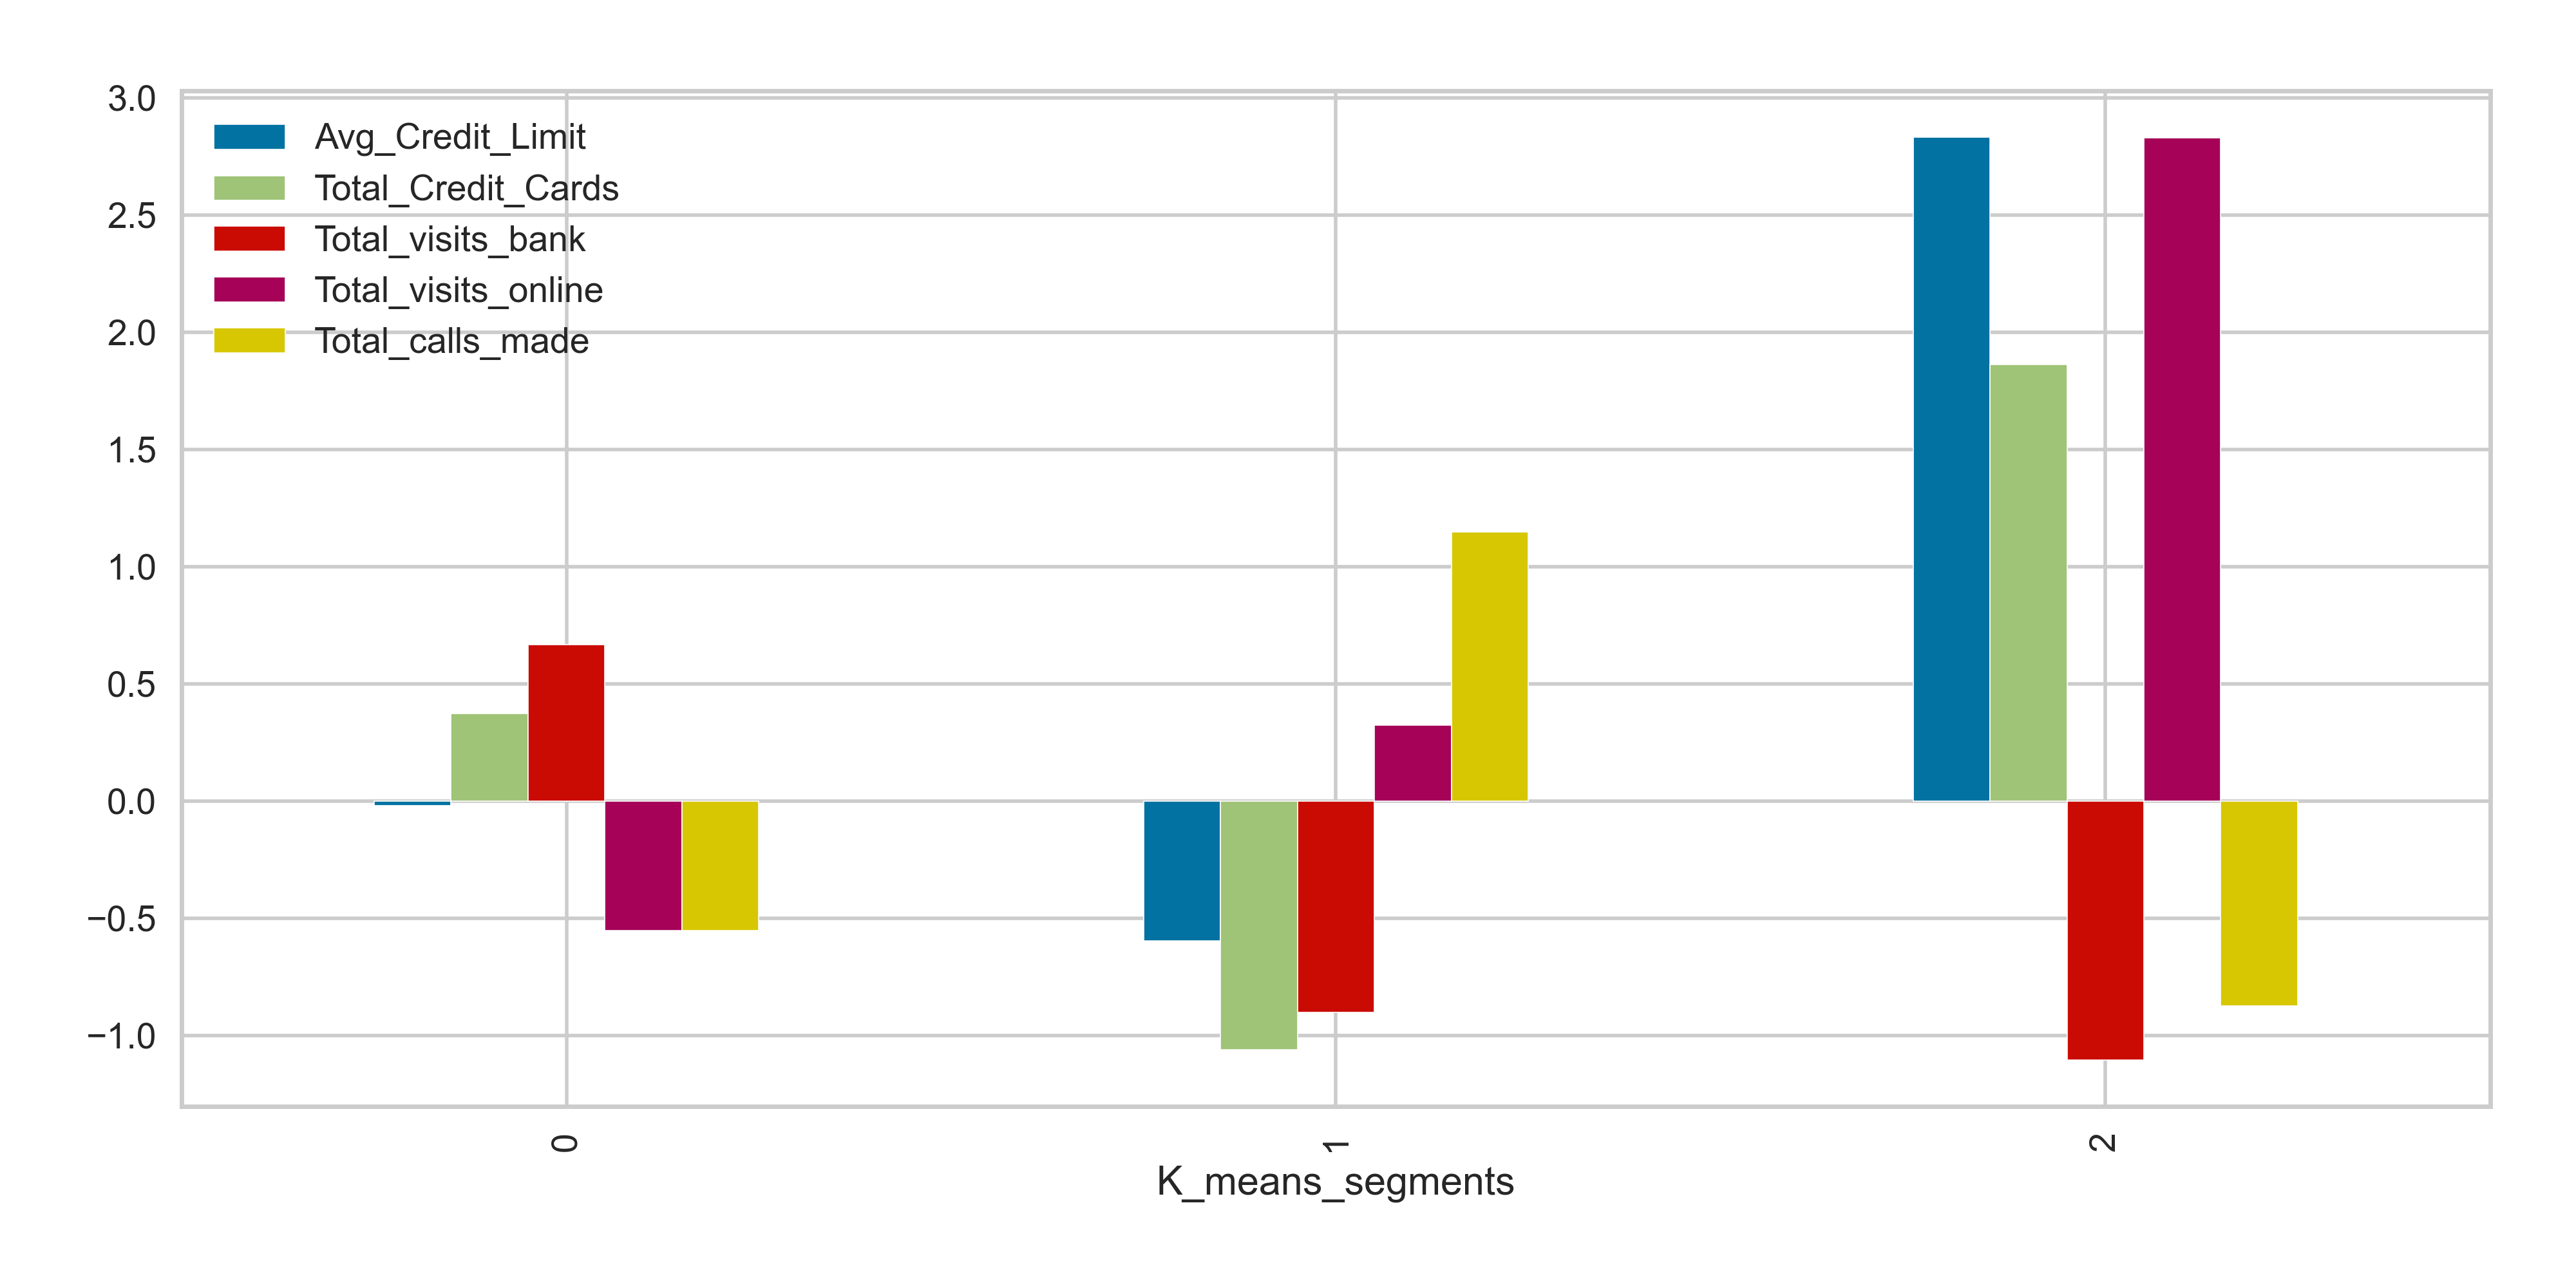
\includegraphics[width=\textwidth]{Kmens_segement_profile_bar.png}
				\caption{Bar plot of means of all the fields across 3 KMeans segment.}
				\label{fig:Kmens_segement_profile_bar.png}
			\end{subfigure}
			\hfill
			\begin{subfigure}[t]{0.49\textwidth}
				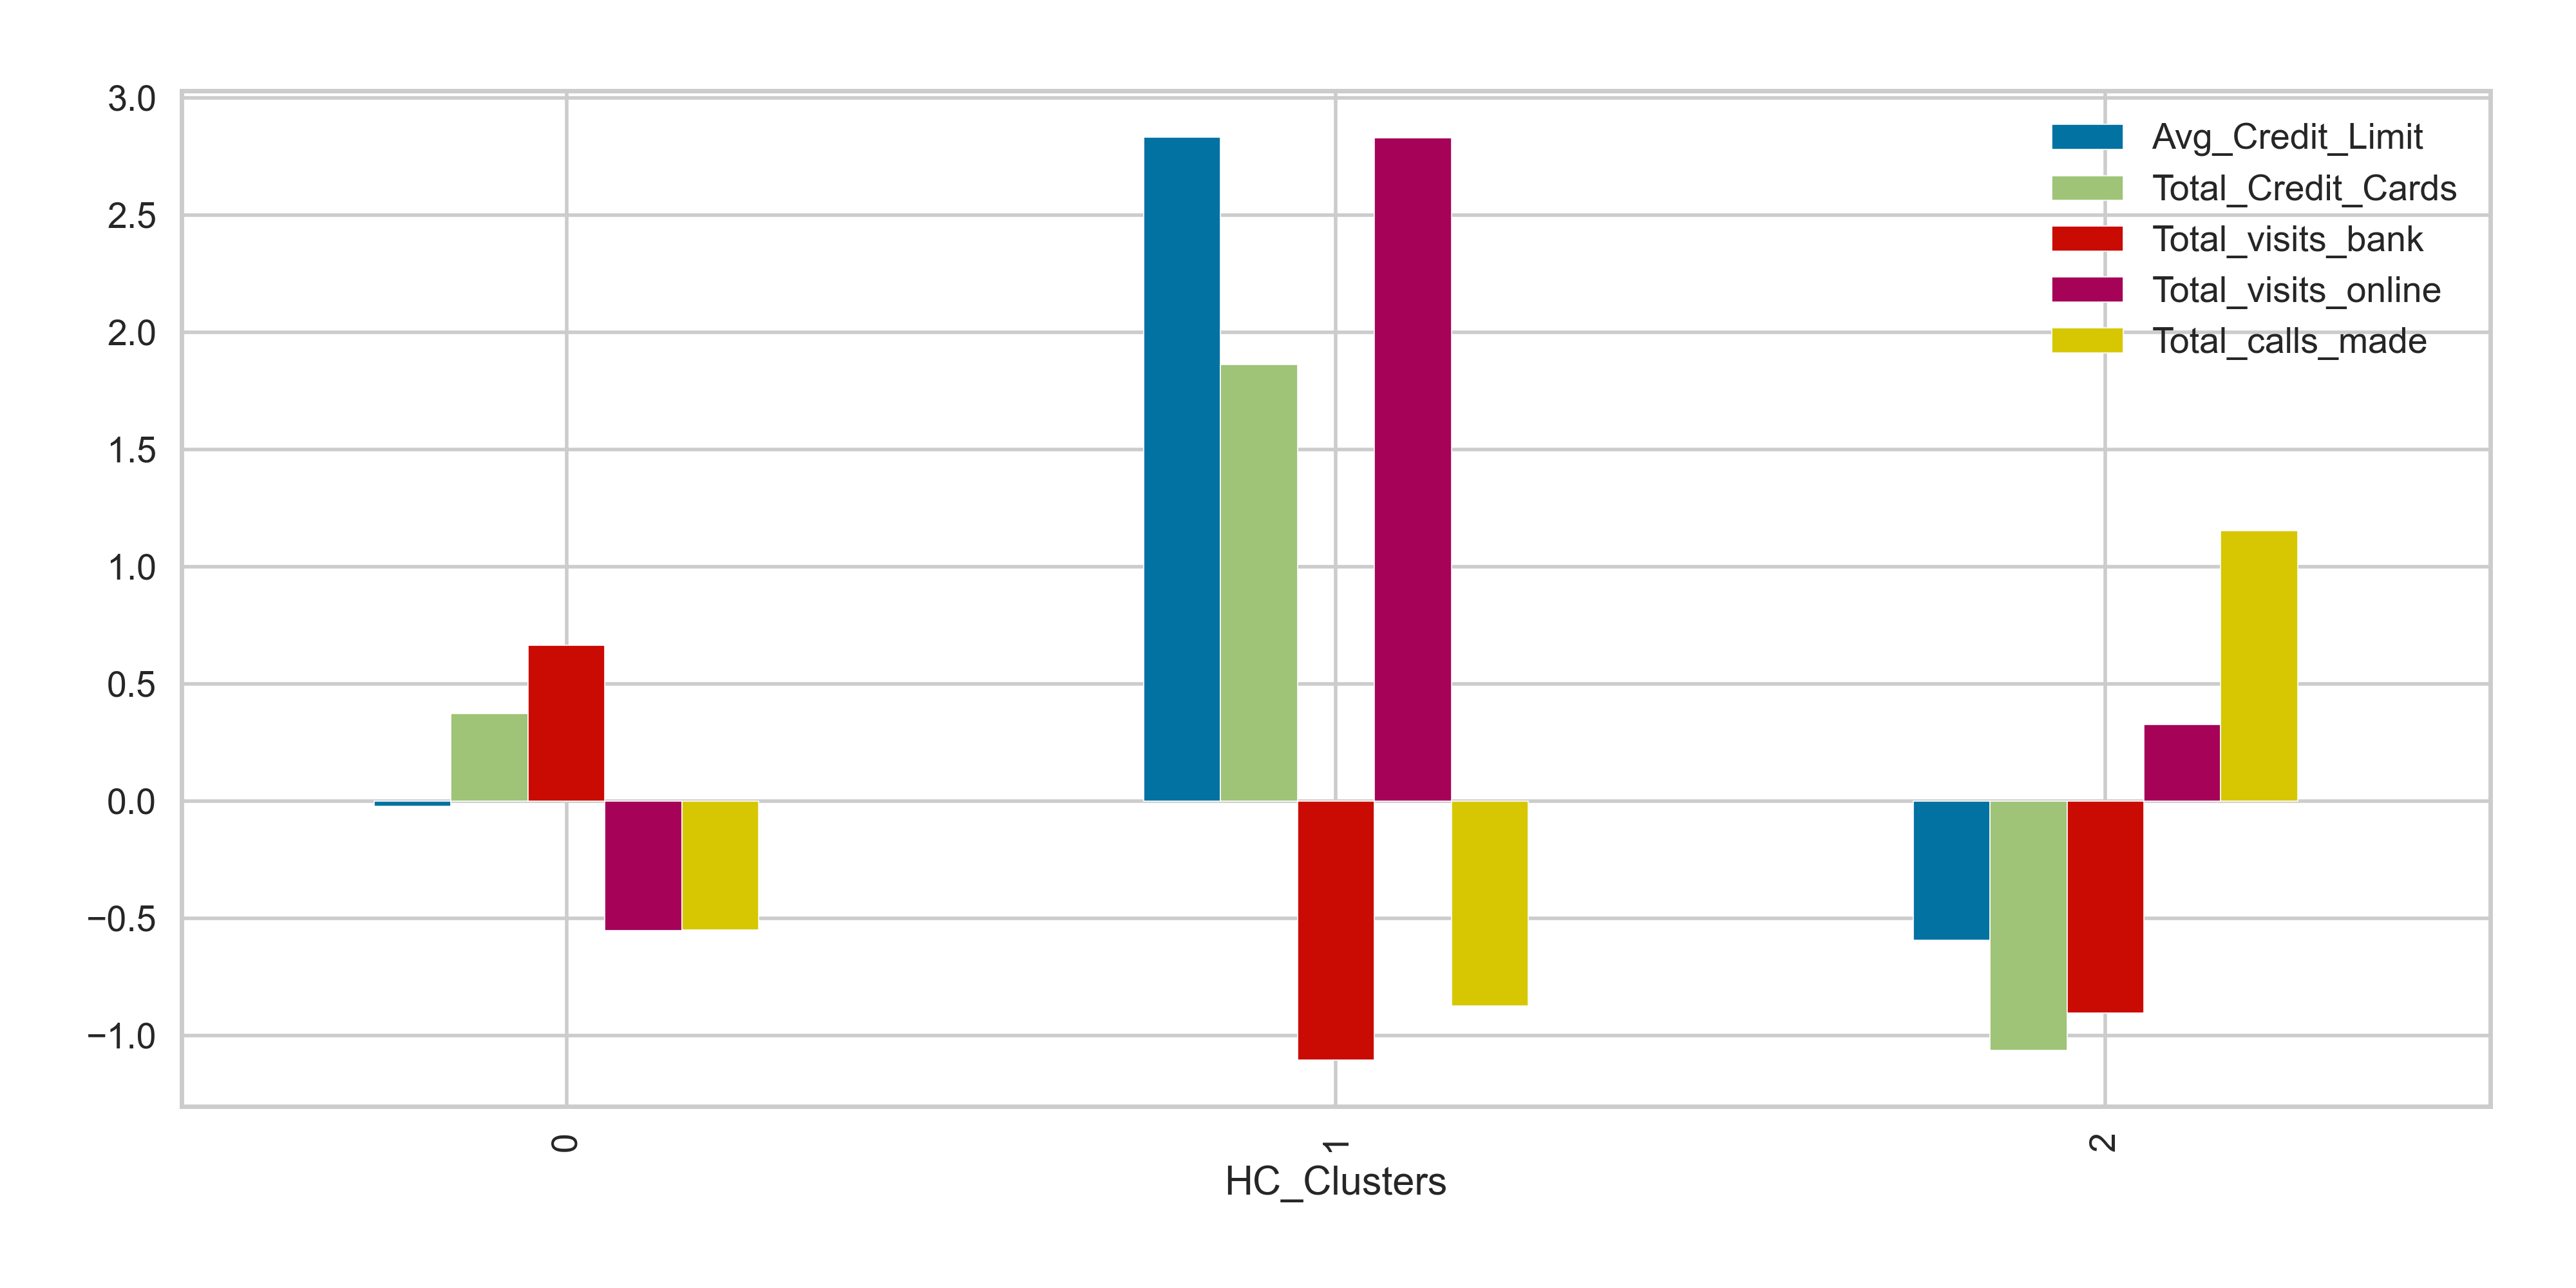
\includegraphics[width=\textwidth]{HC_Clusters_profilr_bar.png}
				\caption{Bar plot of means of all the fields across 3 HC segment.}
				\label{fig:HC_Clusters_profilr_bar.png}
			\end{subfigure}
			\caption{Cluster Method Comparison.}
			\label{fig:Cluster Method Comparision}
		\end{figure}
	
		
		\begin{figure}[h]
			\centering
			\begin{subfigure}[t]{0.49\textwidth}
				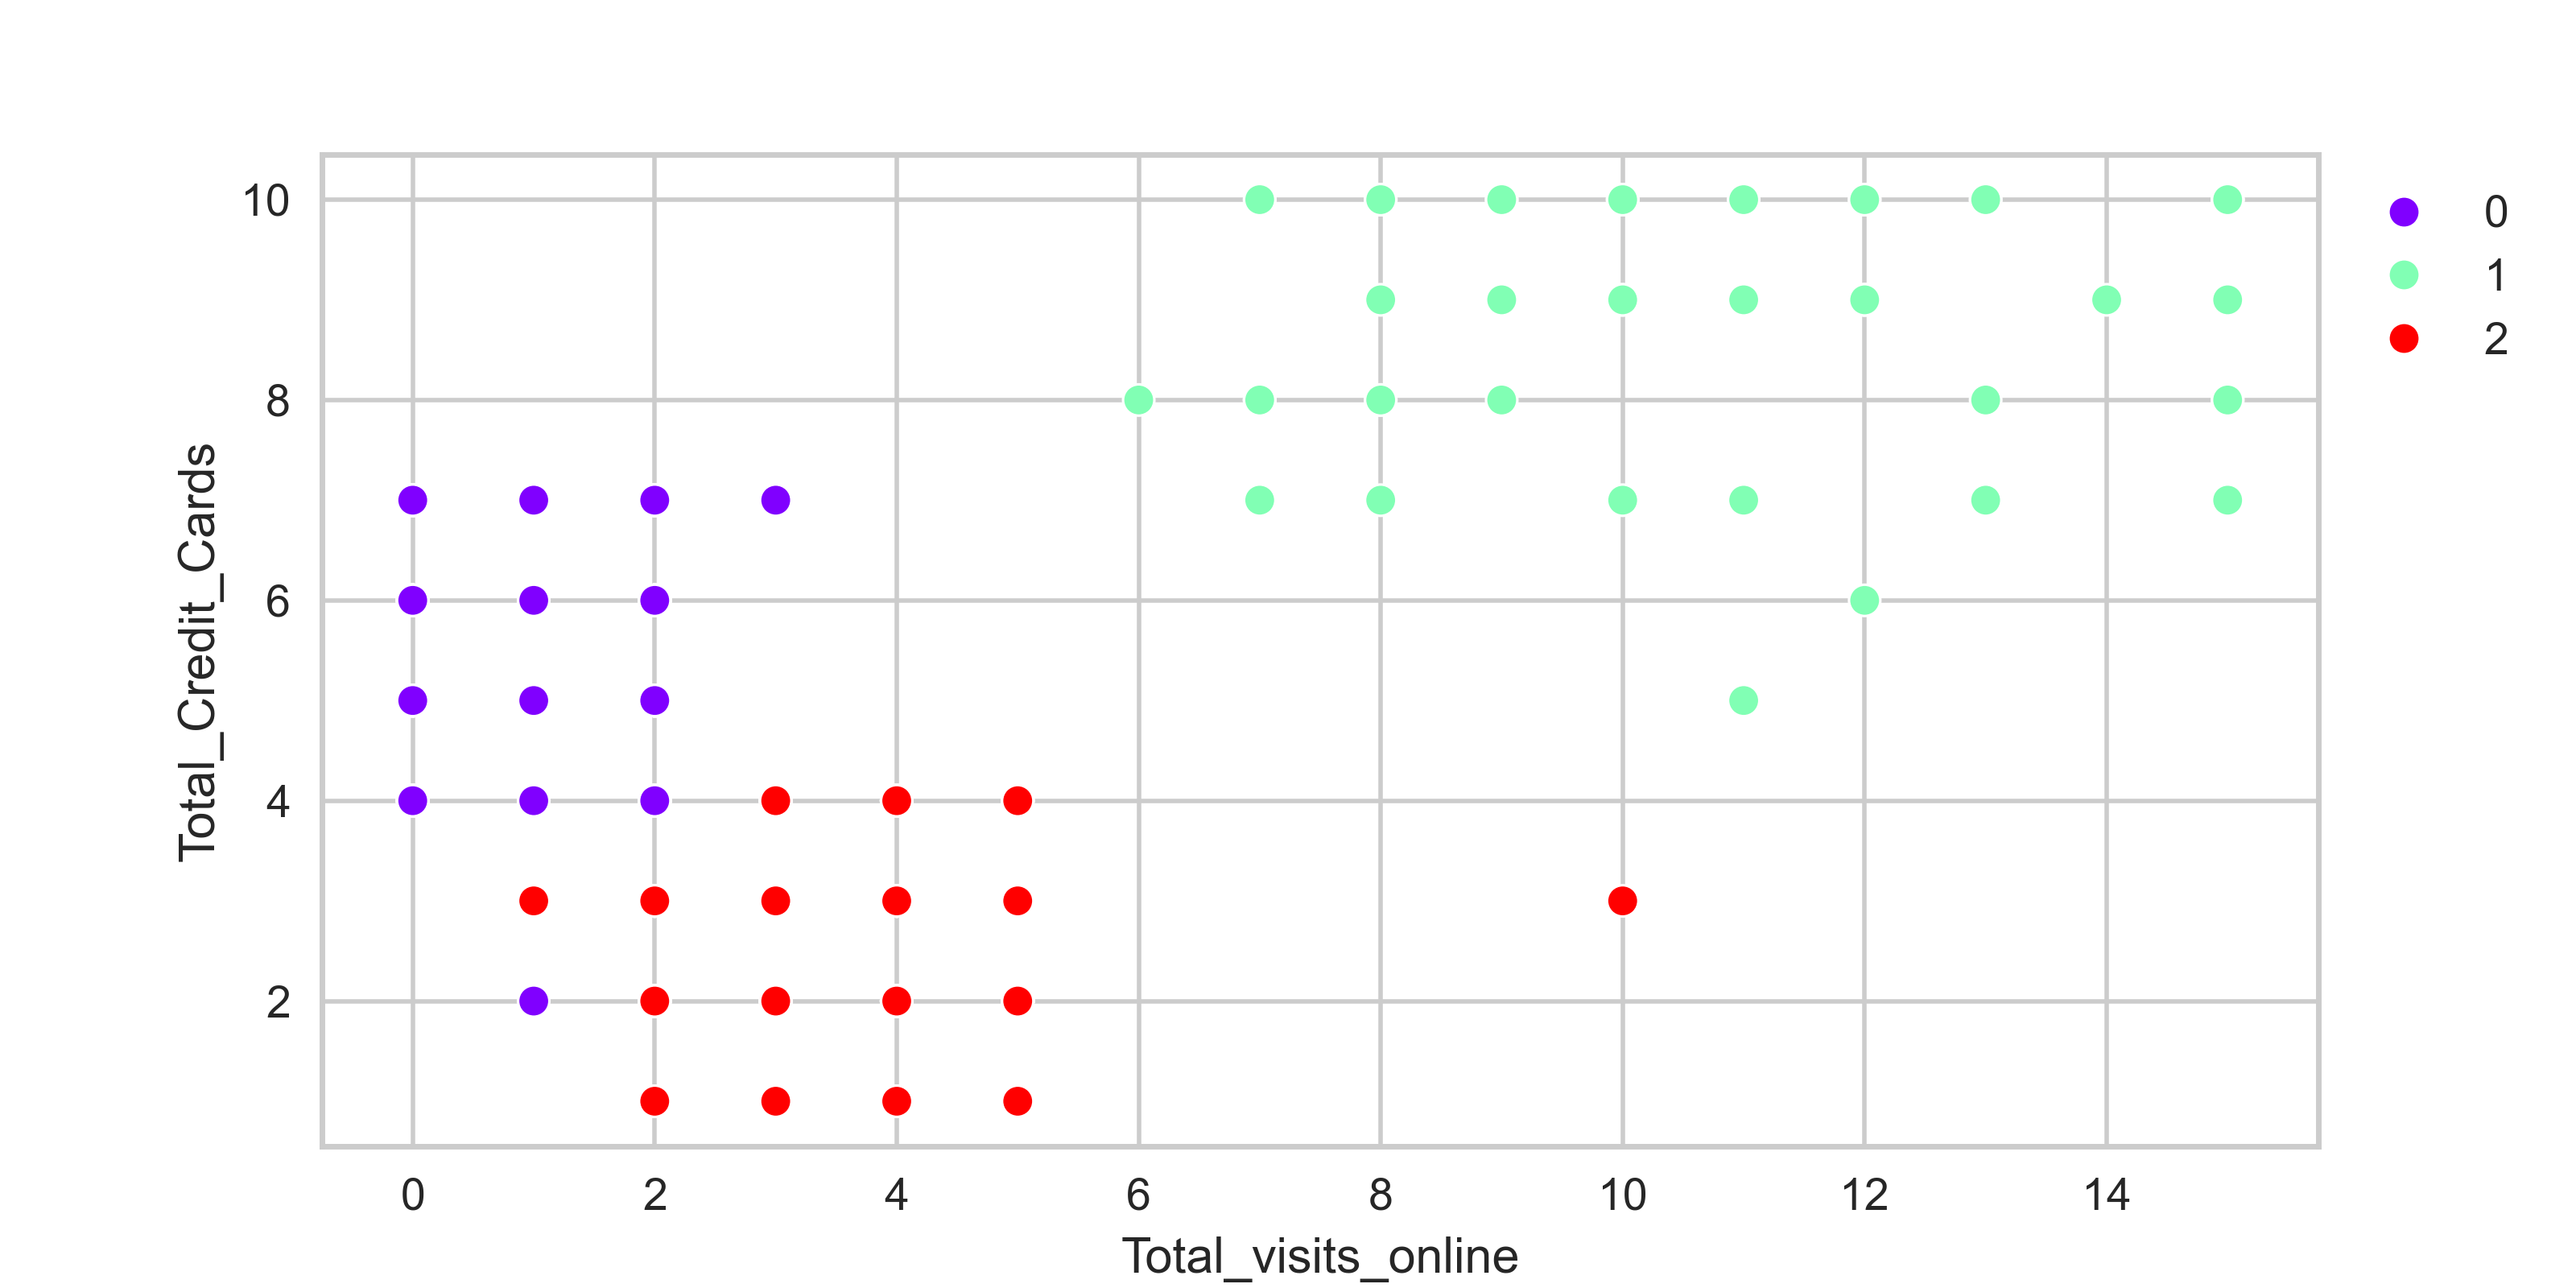
\includegraphics[width=\textwidth]{cluster_vis_cards_vs_online_visits_HC.png}
				\caption{Scatterplot between total Cards and online visits with cluster annoted from HC.}
				\label{fig:cluster_vis_cards_vs_online_visits_HC}
			\end{subfigure}
			\hfill
			\begin{subfigure}[t]{0.49\textwidth}
				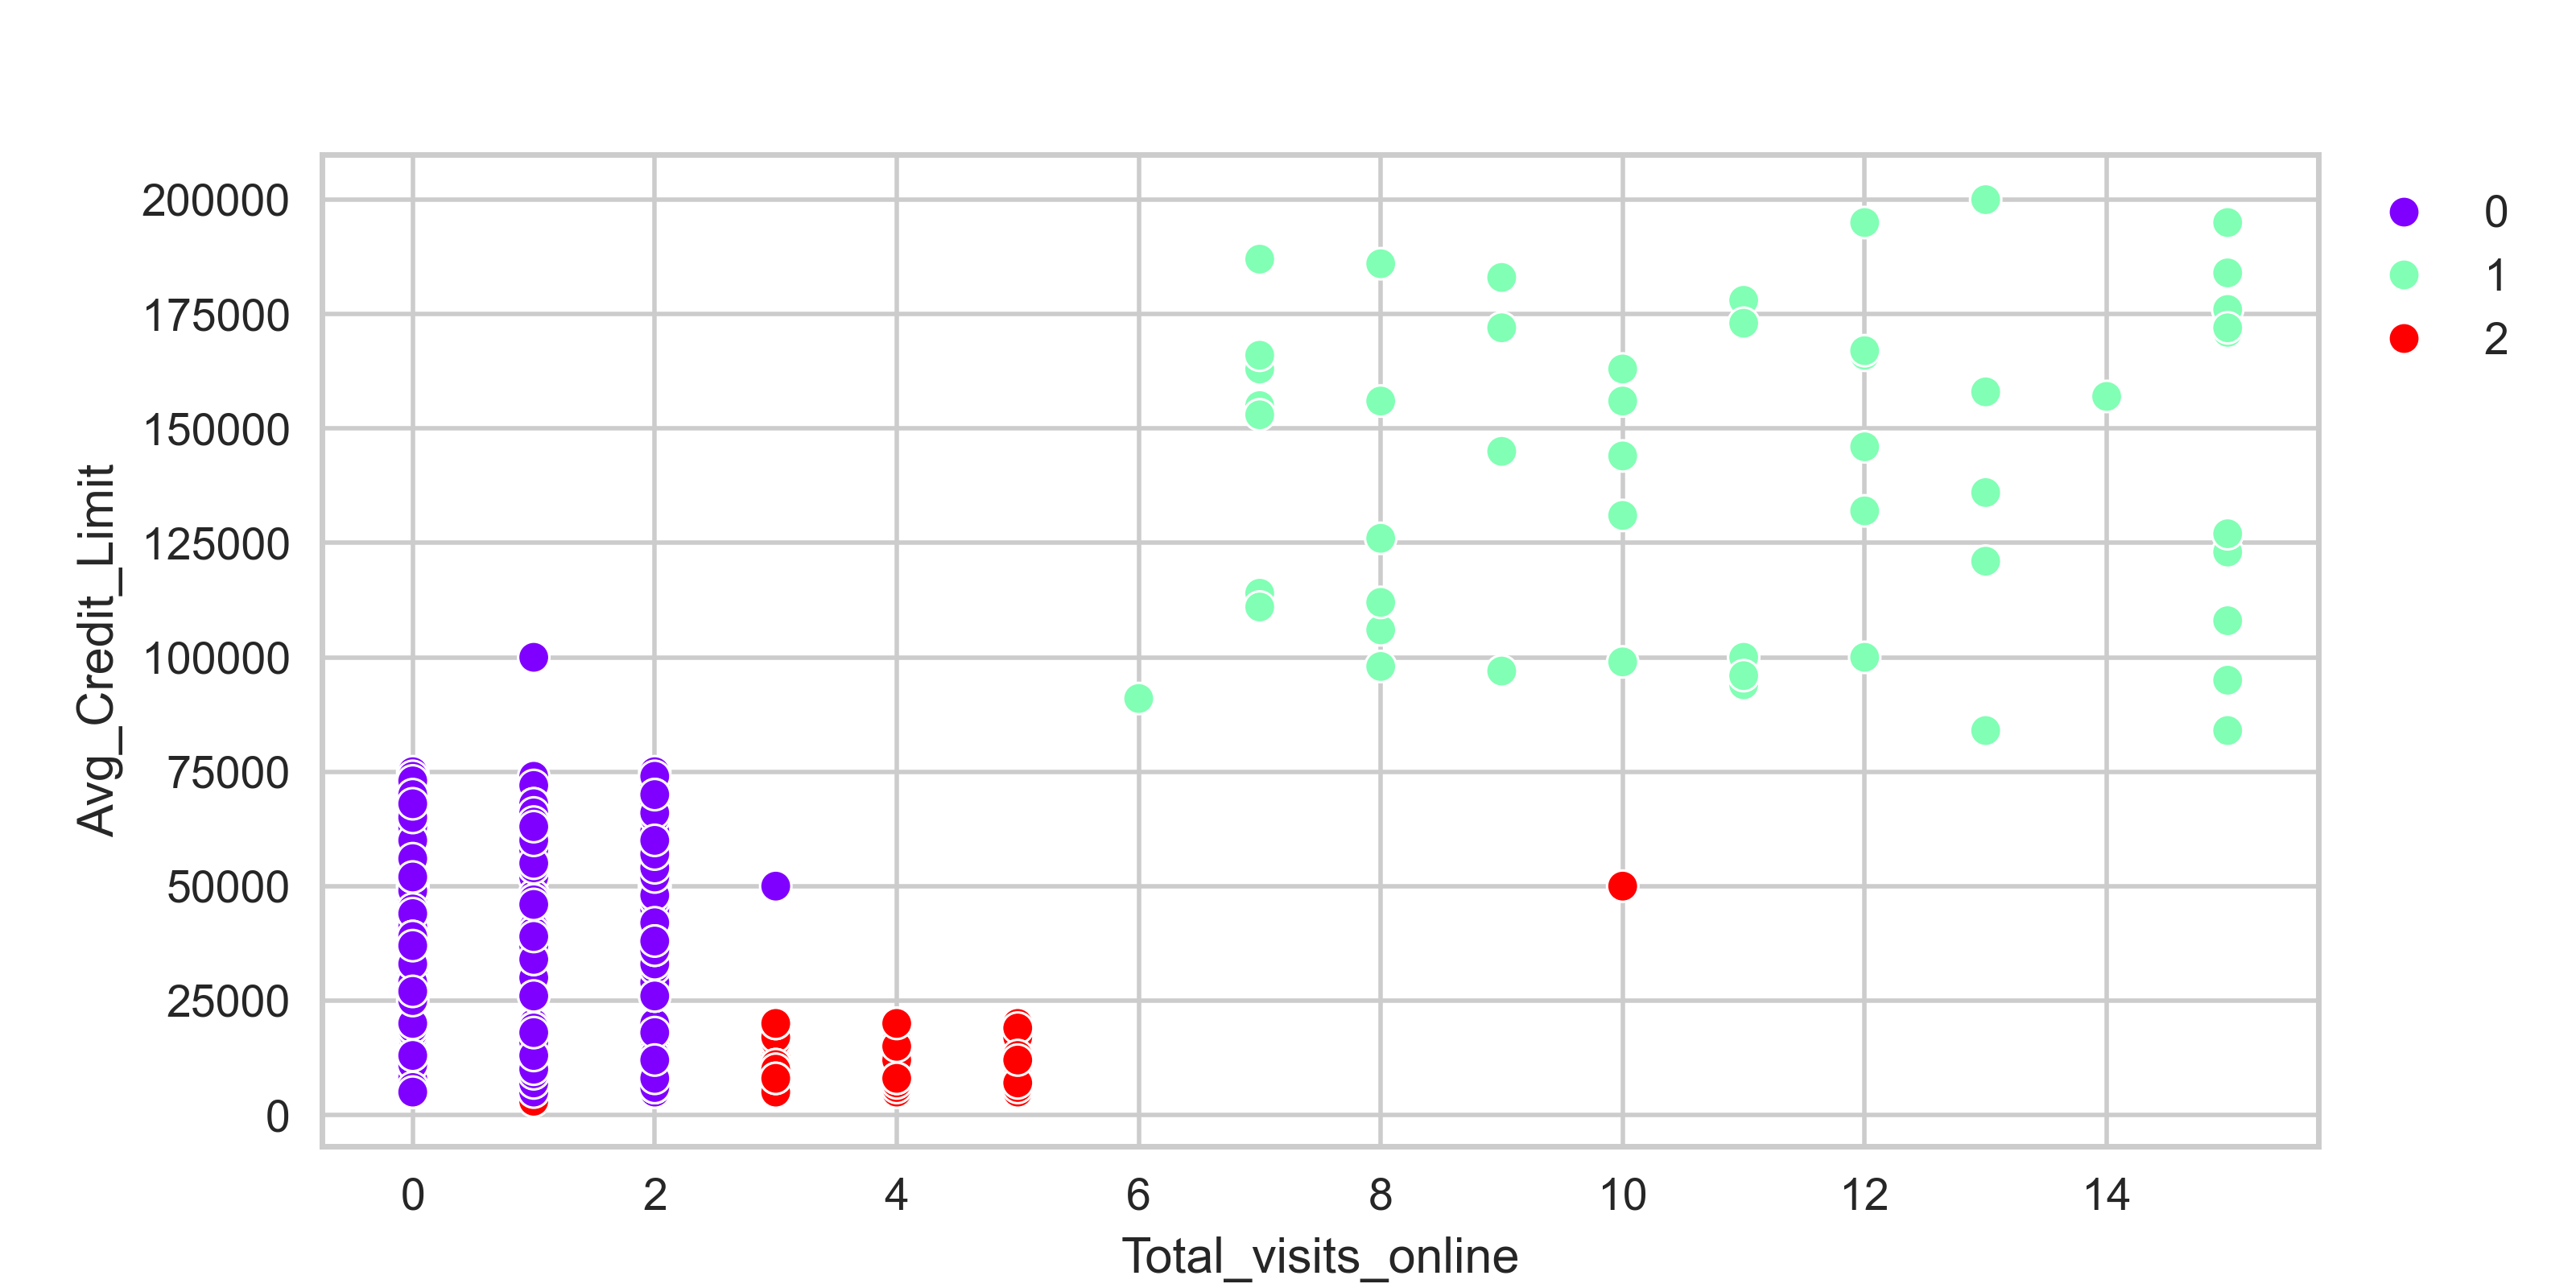
\includegraphics[width=\textwidth]{cluster_vis_credit_vs_online_visit_HC.png}
				\caption{Scatterplot between Credit limit and online visits with cluster annoted from HC.}
				\label{fig:cluster_vis_credit_vs_online_visit_HCg}
			\end{subfigure}
			\begin{subfigure}[t]{0.49\textwidth}
				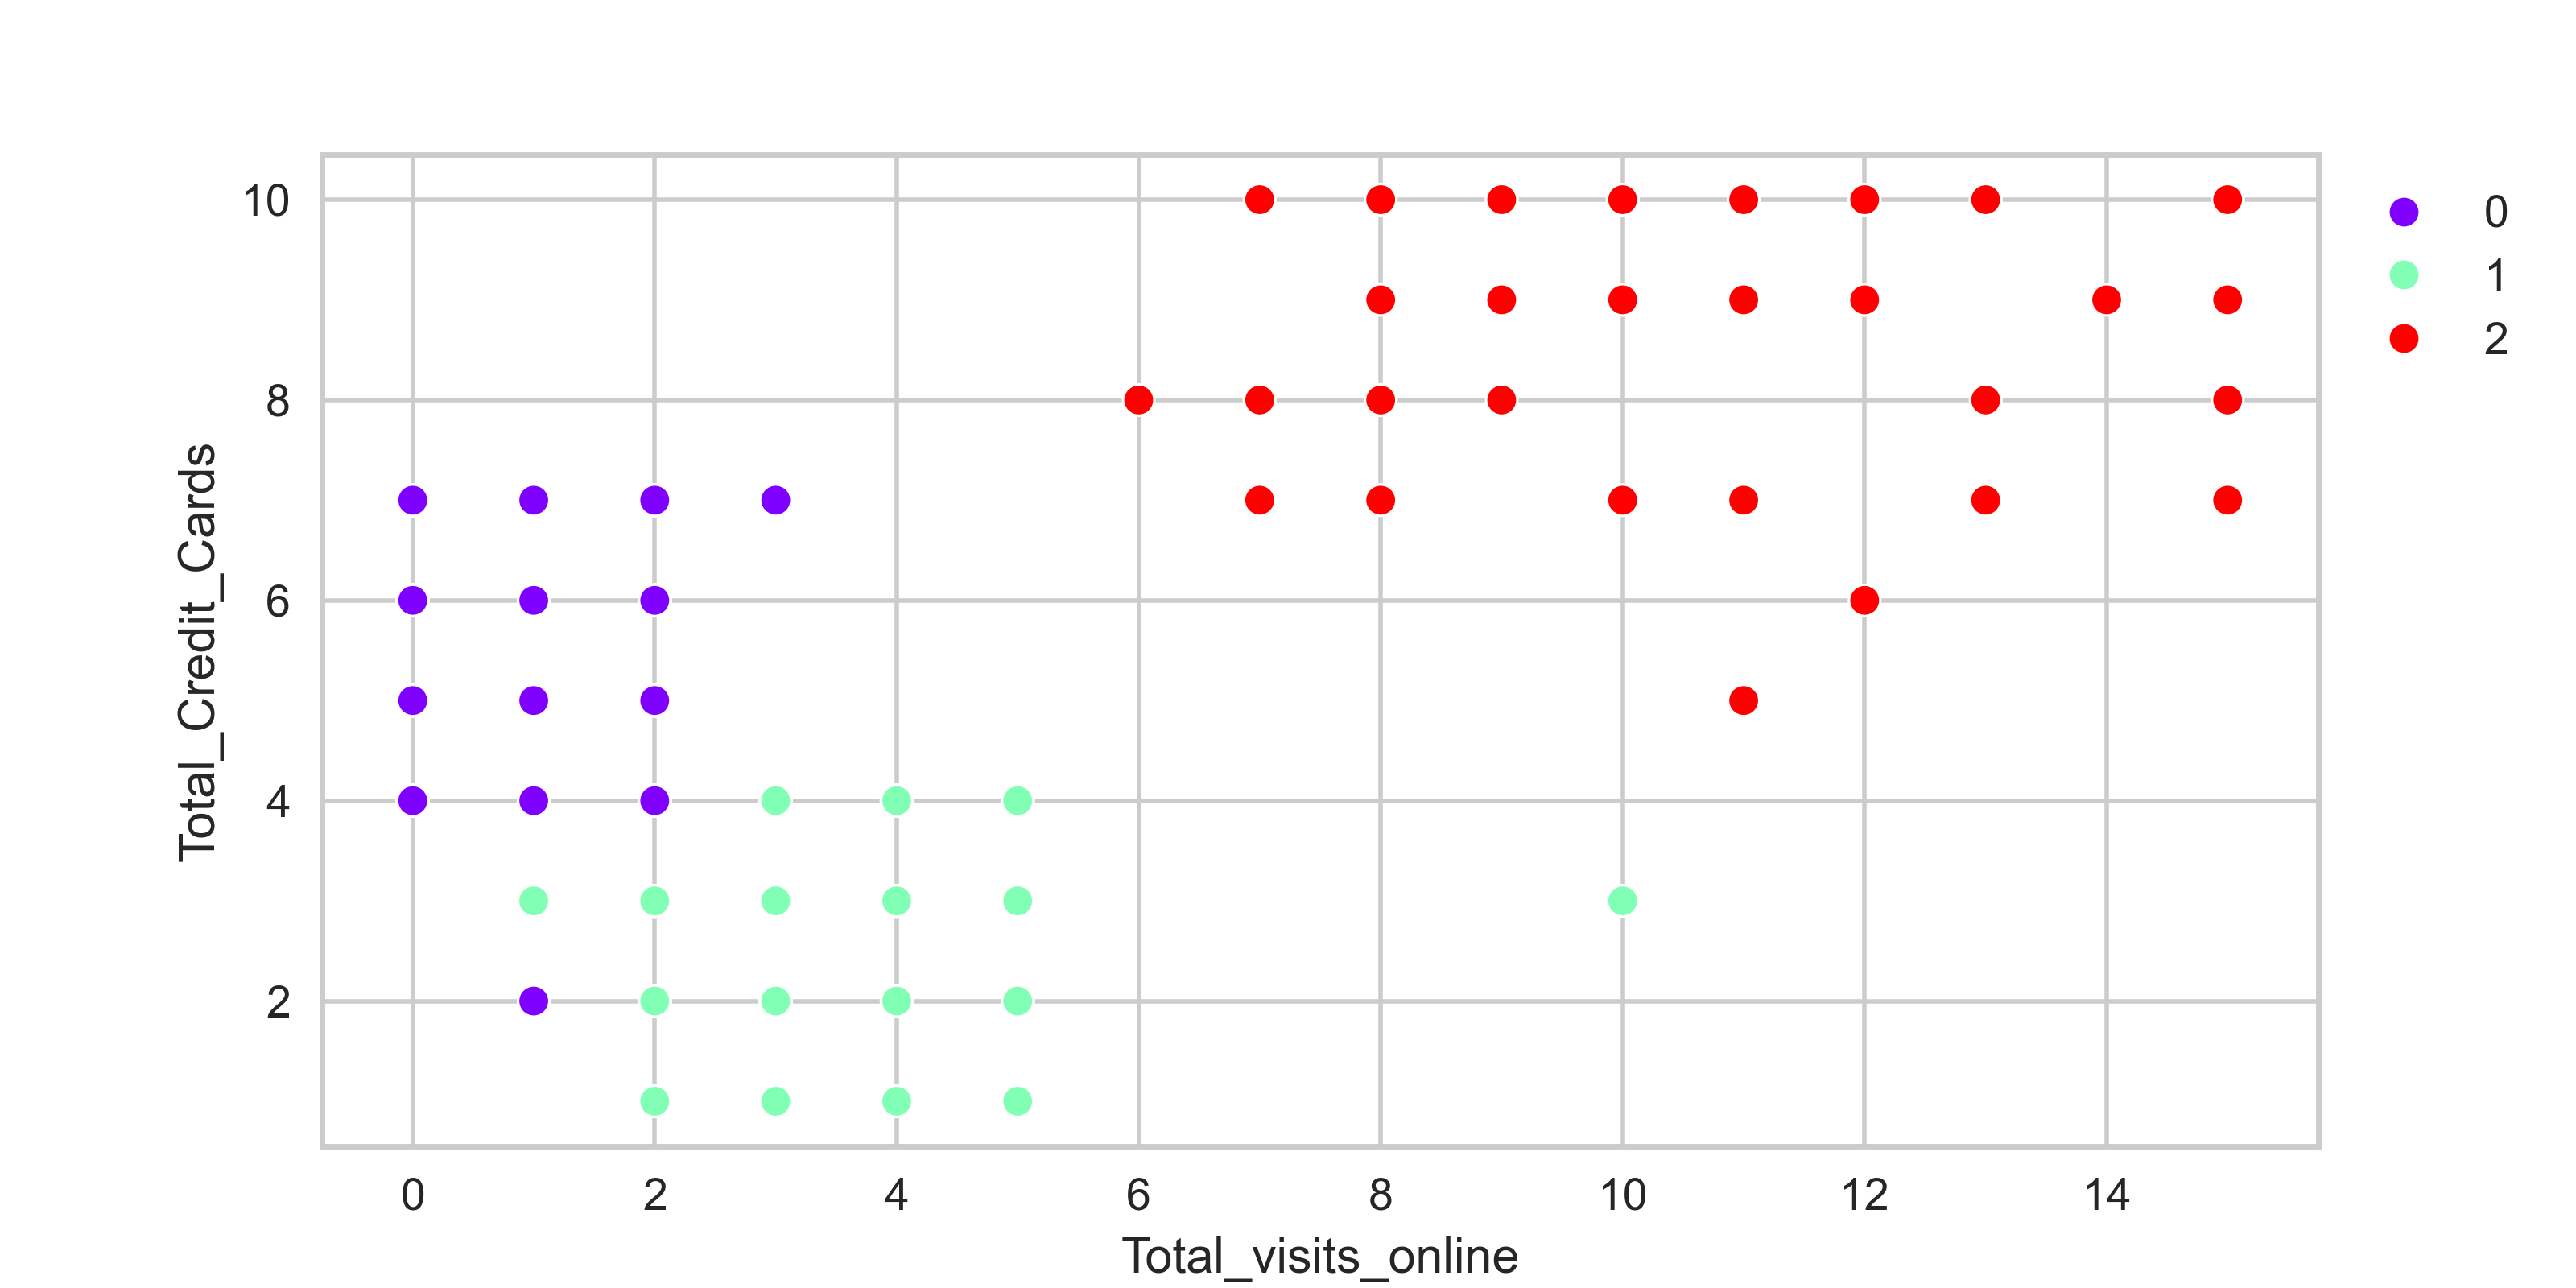
\includegraphics[width=\textwidth]{cluster_vis_cards_vs_online_visits_KM.png}
				\caption{Scatterplot between total Cards and online visits with cluster annoted from Kmeans}
				\label{fig:cluster_vis_cards_vs_online_visits_KM.}
			\end{subfigure}
			\hfill
			\begin{subfigure}[t]{0.49\textwidth}
				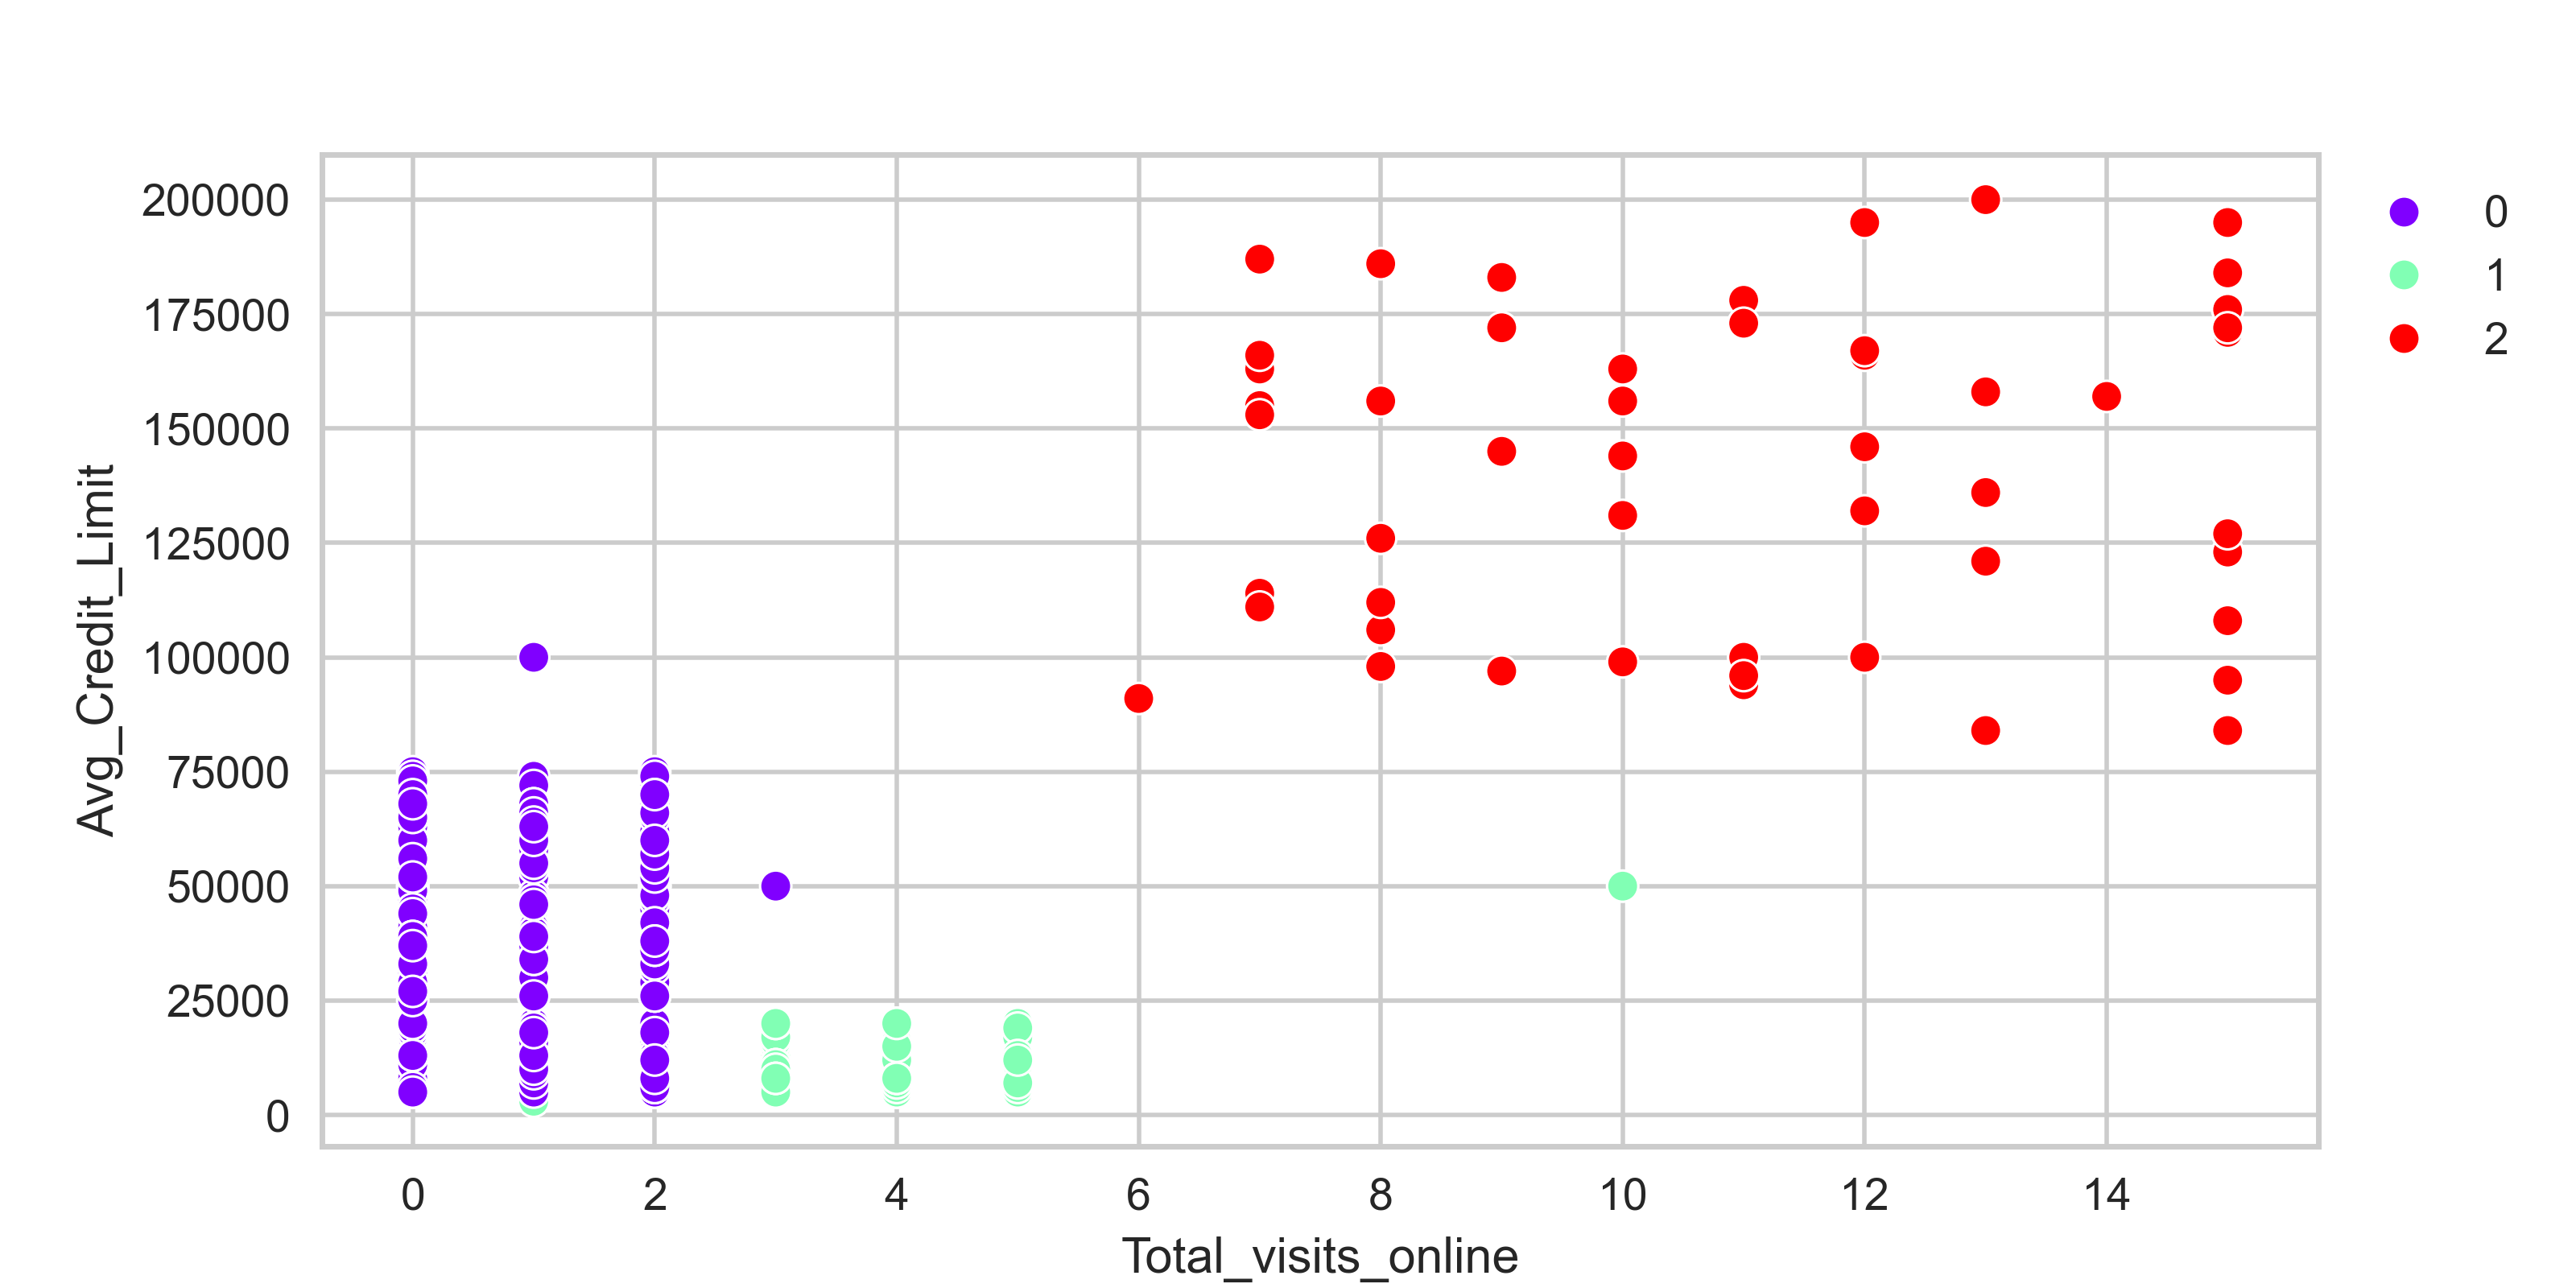
\includegraphics[width=\textwidth]{cluster_vis_credit_vs_online_visit_KM.png}
				\caption{Scatterplot between Credit limit and online visits with cluster annoted from Kmeans.}
				\label{fig:cluster_vis_credit_vs_online_visit_KM}
			\end{subfigure}
			\caption{Cluster Visualization.}
			\label{fig:Cluster Visualization}
		\end{figure}
	\newpage
	\section{Actionable insights and Recommendations}
	\subsection{Actionable insights}
	\begin{itemize}
		\item There are three customers segment for the credit service at AllLife Bank. Let's call them A, B and C. 
		\item Segment A comprise more than 50 \% of customers. They are more likely to visit Bank in person and hold up to 6 or 7 credit cards. Their median credit limit is round 30,000.
		\item Segemt B consists of 7.5 \% of total customers. They make very less phone calls or visit in person. They make higher activity in online mode. Hold higher number of cards and credit limits are usually very high reaching up to 200,000.
		\item Segment C consists of around 34 \% of total customers. They make higher number of phone calls for the services. They have at most 4 credit cards in possession and median credit limit is very less around 12,000.  
		
	\end{itemize}
	
	\subsection{Business Recommendations}
	\begin{itemize}
		\item  The mode of communication for their queries is very distinct in three customer segments we found. Customer service should be fine tailored to adapt to these communication modes (phones, in person and online).
		\item Segment A is the largest. Yet most of them visit bank in person. If we could improve online mode or encourage them to use online mode, we could profit from this segment as higher usage of online mode is correlated with more credit cards.
		\item Section C has 34 \% of total yet they have comparatively few credit cards and limits. Incentives could be offered to customers in these segment to promote credit service. Since they prefer phone calls for query, customer care department should be trained to understand this segment better during calls and could also make some promotions towards call end. 
		\item Segment B only makes 7.5 \% yet they are biggest users in terms of amount. Since they prefer online modes we need to make sure that their user experience is seamless during website or app visit. They have usually high number of credit cards. We need to make sure that apps or websites make access to their card portfolios easily. 
		\item Robust Feed backs mechanism should be developed in all the above modes to address all the three segments and understand if they were satisfied in the customer support.   
		\item The three cluster could be used to identify new incoming customers and serve them accordingly. Simply record their prefer mode of communication, credit limit and number of cards they start to acquire. 
	\end{itemize}
	
\begin{centering}
	\vspace{20pt}
	\subsection*{End of Report\\Submitted by : Haraprasad Dhal}
\end{centering}

\end{document}